\documentclass[10pt,a4paper,twoside,openany,hidelinks]{book}
\usepackage{maths}
\usepackage{stylish}

\usepackage{tkz-graph}
\GraphInit[vstyle = Shade]

\title{Lecture Notes to a course on Lie Algebras \\ \large{Winter 2018, Technion IIT}}
\author{Lectures by Amos Nevo \\ \large Typed by Elad Tzorani}
\date{\today}

\usepackage{lipsum}

\tikzset{EdgeStyle/.style   = {thick,
                               double          = orange,
                               double distance = 1pt}}

\begin{document}
\frontmatter
\frontpage{lie_symmetry}
\tableofcontents
\countlectures
\newpage

\chapter*{Preface}
\addcontentsline{toc}{chapter}{Preface} \markboth{Preface}{}

\section*{Technicalities}
\addcontentsline{toc}{section}{Technicalities} %\markboth{Technicalities}{}

These aren't formal notes related to the course and henceforward there is \emph{absolutely no guarantee} that the recorded material is in correspondence with the course expectations, or that these notes lack any mistakes.\\
In fact, there probably are mistakes in the notes! I would highly appreciate if any comments or corrections were sent to me via email at \href{mailto:tzorani.elad@gmail.com}{tzorani.elad@gmail.com}.\\
Elad Tzorani.

\section*{Course Literature}
\addcontentsline{toc}{section}{Course Literature} %\markboth{Course Literature}{}

The recommended course literature is as follows.

\begin{description}
\item[Humphreys, James E.:] Introduction to Lie algebras and representation theory.

\item[Jacobson, Nathan:] Lie algebras. New York, 1962.
\end{description}

\mainmatter

\part{Lie Algebras}
\chapter{Preliminaries}

The course will be entirely algebraic, with possibly few examples from analysis.%

This will allow us to discuss issues regarding the algebraic properties of Lie algebras.
We might be interested in infinite-dimensional Lie algebras, but in this course we discuss only finite-dimensional algebras.
In this course one of our main goals is a classification theorem for simple Lie algebras.
We assume knowledge in linear algebras and specifically bilinear forms.

\section{Basic definitions}

Let $\FF$ be a field, and $V$ a finite-dimensional vector-space over $\FF$.

\begin{definition}
$V$ is a \stress{generalised $\FF$-algebra} if it comes with a map $m \colon V \times V \to V$ which is bilinear.
\begin{align*}
m\prs{v_1 + v_2, w} &= m\prs{v_1, w} + m\prs{v_2, w} \\
m\prs{v, w_1 + w_2} &= m\prs{v, w_1} + m\prs{v, w_2} \\
m\prs{av, bw} &= abm\prs{v,w}
\end{align*} 
\end{definition}
\begin{example}
Let $V$ be an associative algebra.
Here $m$ is an associative operation which is left and right distributive on addition in $v$.
Equivalently: If we denote $m\prs{v,w} = v \odot w$ then
\begin{align*}
\prs{v \odot w} \odot u &= v \odot \prs{w \odot u} \\
v \odot \prs{u+w} &= v\odot u + v\odot w \\
\prs{u+w}\odot u &= u\odot v + w\odot v
\end{align*}
\end{example}
\begin{remark}
Here associativity means the following.
\[m\prs{v, m\prs{w,u}} = m\prs{m\prs{v,w},u}\]
\end{remark}
\begin{examples}
\begin{enumerate}
\item Every field $k$ is an $\FF$–algebra over any subfield $\FF$.

\item $M_n\prs{k}$ is an $\FF$–algebra.

\item $P_n$, polynomials over $k$ of degree smaller or equal to $n$, is an $\FF$-algebra.
\end{enumerate}
\end{examples}

\begin{definition}
A Lie algebra $L$ over $\FF$ is an $\FF$-algebra, so $\exists m \colon L \times L \to L$, which generally need not be associative, but instead satisfies the following \stress{Jacobi identity},
\begin{align*}
m\prs{X, m\prs{Y,Z}} + m\prs{Z, m\prs{X,Y}} + m\prs{Y,m\prs{Z,X}} = 0
\end{align*}
and additionally, antisymmetry of the multiplication
\[m\prs{X,Y} = -m\prs{Y,X} \text{.}\]
If $\mathrm{char}\FF = 2$ we require $m\prs{X,X} = 0$.
\end{definition}
\begin{notation}
The "multiplication" in $L$ is called \stress{bracket}, and denoted $m\prs{X,Y} = \brs{X,Y}$ ($X$ bracket $Y$).
\end{notation}
\begin{remark}
In these terms we write the Jacobi identity as follows.
\[\brs{X,\brs{Y,Z}} + \brs{Z,\brs{X,Y}} + \brs{Y,\brs{Z,X}} = 0\] 
\end{remark}
\begin{definition}
A \stress{Lie algebra} $L$ is a vector space over $\FF$ with a bilinear map $\brs{,} \colon L \times L \to L$, which is anti-symmetric and satisfies the Jacobi identity.
\end{definition}
\begin{definition}
Given a Lie algebra $L$, a vector subspace $L_0 \subseteq L$ is called a \stress{Lie sub-algebra} if it is closed under brackets. I.e.
\[X,Y \in L_0 \implies \brs{X,Y} \in L_0 \text{.}\]
\end{definition}
\begin{examples}
\begin{enumerate}
\item \emph{Abelian Lie algebras:} The bracket is the zero form.
\[\forall X,Y \in L\colon \brs{X,Y} = 0\]
\end{enumerate}
\end{examples}
\begin{example}
$\FF$ is itself a Lie algebra as well as any $\FF$-vector space $V$ under the bracket \[\forall u,v \in V\colon \brs{u,v} = 0\text{.}\]
\end{example}
\begin{example}
Let $A$ be any associative $\FF$-algebra, and define on $A$ \emph{another} bilinear operation, namely
\[\brs{a,b} = ab - ba \text{.}\]
This is called \stress{the commutator of $a$ and $b$}.
Then $\brs{,} \colon A \times A \to A$.
\begin{exercise}
This bracket satisfies the Jacobi identity, and is anti-symmetric.
\end{exercise}
Given a solution to this exercise, $\prs{A, \brs{,}}$ is a Lie algebra.
\\
In particular, $M_n\prs{k}$ is a Lie algebra under the bracket $\brs{A,B} = AB - BA$.
This algebra is \emph{very important} and is denoted $\gg \ll_n \prs{k}$.
\end{example}
\begin{exercise}
Consider the subspace \[\set{A \in \gg \ll_n\prs{k}}{\mathrm{tr} A = 0} \subseteq \gg \ll_n\prs{k}\text{.}\] Is the subspace a Lie algebra? Yes! Since for any $A,B \in \gg \ll_n\prs{k}$ we have that $\mathrm{tr}\prs{AB} = \mathrm{tr}\prs{BA}$, we get that $\mathrm{tr}\brs{A,B} = 0$.
The sub-Lie-algebra of zero-trace matrices is denoted $\ss\ll_n\prs{k}$.
\end{exercise}
\begin{exercise}[Lie algebras associated with bilinear forms]
Let $V$ be a vector space over $\FF$, and $B \colon V \times V \to \FF$ be a bilinear form.
Assume $B$ is anti-symmetric. Define \[L_B = \set{X \in \mathrm{End}\prs{V}}{B\prs{Xv,w} = -B\prs{v,Xw}}\text{.}\]
Check that $L_B$ is a vector subspace of $\mathrm{End}\prs{V}$.
Consider the bracket operation on $\mathrm{End}\prs{V}$, defined by $\brs{T,S} = TS - ST$.
Is $L_B$ closed under brackets?
\end{exercise}
\begin{solution}
We compute as follows.
\begin{align*}
B\prs{\brs{X,Y}v, w} &= B\prs{\prs{XY - YX}v, w} \\
&= B\prs{XY v, w} - B\prs{YXv,w} \\
&= -B\prs{Yv,Xw} + B\prs{Xv,Yw} \\
&= B\prs{v,YXw} -B\prs{v,XYw} \\
&= B\prs{v, \prs{YX - XY}w} \\
&= -B\prs{v, \brs{X,Y}w}
\end{align*}
In conclusion, $L_B$ is a sub-Lie-algebra of $\mathrm{End}\prs{V}$, the Lie algebra associated with the form $B$.
\end{solution}
\begin{exercise}
Let $S$ be a symmetric bilinear form, and let \[L_S = \set{X \in \mathrm{End}\prs{V}}{S\prs{Xv, w} = -S\prs{v,Xw}}\text{.}\]
Then again, $L_S$ is a Lie sub-algebra.
\end{exercise}
\begin{examples}[Sub-algebras of $\gg \ll_n\prs{\FF}$]
\begin{enumerate}
\item
\[\tt\prs{n,\FF} = \set{\pmat{a_{11} & & a_{i,j} \\ & \ddots & \\ 0 & & a_{nn}}}{a_{ij} \in \FF}\]
is closed under the bracket operation, for if $A,B \in \tt\prs{n,\FF}$ then $AB \in \tt\prs{n,\FF}$ and so $AB - BA \in \tt\prs{n,\FF}$.
\item \[\nn\prs{n,\FF} = \set{\pmat{0 & & a_{i,j} \\ & \ddots & \\ 0 & & 0}}{a_{ij} \in \FF}\]
is a Lie sub-algebra of $\tt\prs{n,\FF}$.
\item \[\dd\prs{n,\FF} = \set{\pmat{a_1 & & 0 \\ & \ddots & \\ 0 & & a_n}}{a_i \in \FF}\]
an abelian sub-algebra. 
\end{enumerate}
\end{examples}
\section{Structure constants}
Let $L$ be a Lie algebra and let $X_1, \ldots, X_n$ be a basis of $L$, Then the bracket operation is completely determined by the structure constants with respect to the basis.
\[\brs{X_i, X_j} = \sum_{k=1}^n c_k^{i,j} X_k\]
The \stress{structure constants} $c_k^{i,j}$ contain full information on the bracket operation of course. These satisfy two properties associated with anti-symmetry and the Jacobi identity of the brackets.
The property associated to anti-symmetry is $c_k^{i,j} = -c_k^{j,i}$. The other property (associated to the Jacobi identity) is left as an \textbf{\textrm{Exercise}}.
\begin{example}
\[\gg \ll_n\prs{\FF} = \mathrm{span}\set{E_{i,j}}{1 \leq i,j\leq n}\]
In the basis $E_{ij}$ the structure constants are very simple. We have the following.
\[\brs{E_{i,j}, E_{k,l}} = \delta_{j,k}E_{i,l} - \delta_{l,i}E_{k,j}\]
Hence all the structures constants are $1$ or $-1$.
\end{example}
\begin{definition}
Let $L_1, L_2$ be Lie algebras. A \stress{Lie algebra homomorphism} between $L_1$ and $L_2$ is a linear map $T \colon L_1 \to L_2$ satisfying
\[T\brs{X,Y} = \brs{TX, TY}\text{.}\]
\end{definition}
\begin{definition}
Let $L$ be a Lie algebra. A sub-space $I \subseteq L$ is called a \stress{Lie-ideal} of $L$ if for all $X \in L$ and $Y \in I$, we have that $\brs{X,Y} \in I$. This is written also by 
\[\brs{L,I} = \mathrm{span}\set{\brs{X,Y}}{X \in L, Y \in I} \subseteq I \text{.}\]
\end{definition}
\begin{definition}
Let $L$ be a Lie algebra and $L_0 \subseteq L$ be a sub-space. The \stress{Lie normaliser} of $L_0$ is
\[N\prs{L_0} = \set{X \in L}{\brs{X,L_0} \subseteq L_0}\text{.}\]
The \stress{Lie centraliser} of $L_0$ is
\[Z\prs{L_0} = \set{X \in L}{\brs{X,L_0} = 0} \text{.}\]
\end{definition}
\begin{definition}
Let $L$ be a Lie algebra. If $\brs{X,Y} = 0$ one says that $X$ and $Y$ commute.
We sometimes refer to the bracket as the commutator.
\end{definition}
\begin{example}
Two sub-spaces $L_1, L_2 \subseteq L$ of a Lie algebra commute if their commutators are zero. I.e.
\[\brs{L_1, L_2} = 0 \text{.}\]
\end{example}
\begin{remark}
Although we have linearity of the bracket, we do need to take the span in the above example. If we take $X,X' \in L_1$ and $Y,Y' \in L_2$ we can't always express $\brs{X,Y} + \brs{X',Y'}$ as a bracket of two elements, although it certainly is in the span.
\end{remark}
\section{Linear representations}
\begin{definition}
A \stress{linear representation} of a Lie algebra $L$ over $\FF$ is a Lie-algebra homomorphism $T \colon L \to \mathrm{End}(V) \cong \gg \ll_n\prs{\FF}$ where $V$ is an $n$-dimensional vector space over $\FF$.
\end{definition}
\begin{remark}
The bracket operation on $\mathrm{End}(V)$ is the usual one, namely $\brs{A,B} = AB - BA$.
\end{remark}
Let us define another large collection of Lie algebras. First, let $A$ be a generalised $\FF$–algebra, and denote $m\prs{a,b} = a \odot b$.\\
\begin{definition}
A \stress{derivation} of the generalised algebra $A$ is a linear map $\delta \colon A \to A$ satisfying the following property.
\begin{align*}
\delta \prs{ a \odot b} = \delta\prs{\alpha} \odot b + a \odot \delta\prs{b}
\end{align*}
\end{definition}
\begin{definition}
\[\mathrm{Der}\prs{A} \ceq \set{\delta \in \mathrm{End}\prs{A}}{\text{$\delta$ is a derivation.}}\]
\end{definition}
\begin{remark}
$\mathrm{Der}(A)$ is clearly a linear sub-space of $\mathrm{End}(A)$.
Now, if $\delta_1$ and $\delta_2$ are derivations, $\delta_1 \circ \delta_2$ is \emph{not} a derivation, usually.
But, $\brs{\delta_1, \delta_2} = \delta_1 \circ \delta_2 - \delta_2 \circ \delta_1$ \emph{is} in fact a derivation.
\end{remark}
\begin{conclusion}
$\mathrm{Der}(A)$, with the bracket inherited from $\mathrm{End}(A)$ is a Lie algebra.
\end{conclusion}
\begin{proof}
We compute the following.
\begin{align*}
\brs{\delta_1, \delta_2}\prs{a \odot b} &= \prs{\delta_1 \circ \delta_2 - \delta_2 \circ \delta_1}\prs{a \odot b} \\
&= \delta_1 \circ \delta_2\prs{a \odot b} - \delta_2 \circ \delta_1 \prs{a \odot b} \\
&= \delta_1 \prs{\delta_2\prs{a}\odot b + a\odot \delta_2\prs{b}} - \delta_2 \prs{\delta_1\prs{a}\odot b + a\odot\delta_1\prs{b}} \\
&= \delta_1 \delta_2 \prs{a} \odot b + \delta_2\prs{a} \odot \delta_1\prs{b} + \delta_1\prs{a}\odot \delta_2\prs{b} + a\odot \delta_1\delta_2\prs{b} \\ &- \prs{\delta_2 \delta_1\prs{a} \odot b + \delta_1 \prs{a} \odot \delta_2 \prs{b} + \delta_2\prs{a} \odot \delta_1\prs{b} + a\odot \delta_2 \delta_1\prs{b}} \\
&= \prs{\delta_1 \delta_2 - \delta_2 \delta_1} \prs{a} \odot b + a\odot \prs{\delta_1 \delta_2 - \delta_2 \delta_1}\prs{b}
\end{align*}
\end{proof}
\begin{example}
\begin{enumerate}
\item If $A$ is an associative algebra, then $\mathrm{Der}(A)$ is a Lie algebra, $\mathrm{Der}(A) \subseteq \mathrm{End}(A)$. $\mathrm{Der}(A)$ is a sub-Lie-algebra of $\mathrm{End}(A)$ under bracket of linear transformations.
\item A Lie algebra is a generalised algebra and so $\mathrm{Der}(L)$ is another Lie algebra.
\end{enumerate}
\end{example}
\begin{fact}[important]
There is a very natural collection of derivations of any Lie algebras.
For each $x \in L$, let us define a linear transformation denoted $\mathrm{ad}(x) \colon L \to L$ (this stands for "adjoint") via
$\mathrm{ad}(x)(y) = \brs{x,y}$. (This is linear from the bi-linearity of the bracket)
In fact, $\mathrm{ad}(x)$ is a derivation of $L$. Namely,
\[\mathrm{ad}(x)\prs{\brs{y,z}} = \brs{\mathrm{ad}(x)y,z} + \brs{y, \mathrm{ad}(x)(z)}\text{.}\]
Indeed,
\begin{align*}
\mathrm{ad}(x)\prs{\brs{y,z}} &= \brs{x,\brs{y,z}} \\
&= \brs{\mathrm{ad}(x)y, z} + \brs{y, \mathrm{ad}(x)z} \\
&= \brs{\brs{x,y},z} + \brs{y,\brs{x,z}}
\end{align*}
which is an identity as a consequence of the Jacobi identity.
\end{fact}
\begin{conclusion}
The set $\set{\mathrm{ad}(x)}{x \in L} \subseteq \mathrm{Der}(L)$ is a sub-algebra.
We have the map $x \mapsto \mathrm{ad}(x)$ which is obviously linear (from bi-linearity of the bracket).
So, $\mathrm{ad}(L) \ceq \set{\mathrm{ad}(x)}{x \in L}$ is a linear sub-space.
In fact it is a Lie sub-algebra of $\mathrm{Der}(L)$.
\end{conclusion}
\begin{proof}
We have to show that $\brs{\mathrm{ad}(x),\mathrm{ad}(y)} = \mathrm{ad}(x)\mathrm{ad}(y) - \mathrm{ad}(y)\mathrm{ad}(x)$ is in the space $\mathrm{ad}(L)$. But, actually $\brs{\mathrm{ad}(x), \mathrm{ad}(y)} = \mathrm{ad}\brs{x,y}$, as the following proposition states.
\begin{proposition}
$\mathrm{ad} \colon L \to \mathrm{Der}(L)$
is a Lie algebra homomorphism.
\end{proposition}
\begin{proof}
Let us compute.
\begin{align*}
\brs{\mathrm{ad}(x), \mathrm{ad}(y)}\prs{z} &= \mathrm{ad}\prs{x} \mathrm{ad}\prs{y}\prs{z} - \mathrm{ad}\prs{y}\mathrm{ad}\prs{x}\prs{z} \\
&= \brs{x,\brs{y,z}} - \brs{y,\brs{x,z}} \\
&\stackrel{\star}{=} \brs{\brs{x,y},z} \\
&= \mathrm{ad}\brs{x,y}\prs{z}
\end{align*}
where the $\star$ is given from the Jacobi identity.
\end{proof}
In conclusion, $\mathrm{Der}(L)$ is a Lie sub-algebra of $\mathrm{End}(L)$ under bracket, and $\mathrm{ad} \colon L \to \mathrm{Der}(L) \subseteq \mathrm{End}(L)$ is a linear representation of the Lie algebra $L$ with the image being $\mathrm{ad}(L) = \set{\mathrm{ad}(x)}{x \in L}$.
\end{proof}
\begin{example}
Given $L_0 \subseteq L$ a sub-space. Then
$N\prs{L_0} = \set{x}{\brs{x,L_0} \subseteq L_0}$ is the set of elements $x$ such that the linear transformation $\mathrm{ad}\prs{x}$ leaves the subspace $L_0$ invariant. $N_L\prs{L_0}$ is a Lie sub-algebra, and if $L_0$ is a Lie sub-algebra, then $L_0$ is an ideal of $N_L\prs{L_0}$.
\end{example}
\begin{example}
The condition $\brs{X,Y} = 0$ means $Y \in \ker\prs{\mathrm{ad}(x)}$ or equivalently $x \in \ker\prs{\mathrm{ad}(y)}$. Therefore
\begin{align*}
Z\prs{L_0} &= \set{x \in L}{\brs{x,L_0} = 0} \\
&= \set{x \in L}{L_0 \subseteq \ker\prs{\mathrm{ad}(x)}} \text{.}
\end{align*}
$Z\prs{L_0}$ is a Lie sub-algebra of $L$, the Lie sub-algebra of elements commuting with every $x \in L_0$.
\end{example}
\begin{remark}
If $L_0 \subseteq L$ is a Lie sub-algebra, then $N\prs{L_0}$ is the largest sub-algebra such that $L_0$ is is an ideal in it.
\end{remark}

\begin{remark}
$Z_L(L)$ is the center of $L$, and an ideal.%
Indeed, if $z \in Z\prs{L}$, and $x \in L$, then $\ad\brs{x,z} = \ad x \ad z - \ad z - \ad x$ and $L \subseteq \ker \ad z$, so $L \subseteq \ker \ad \brs{x,z}$, so $\brs{x,z} \in Z\prs{L}$ and $Z(L)$ is an ideal.
\end{remark}
\section{Sub-algebras and ideals}
\begin{remark}
\begin{enumerate}
\item If $L_1$ and $L_2$ are Lie sub-algebras, then $L_1 + L_2$ generally \emph{is not}!
\item Suppose $I = L_1$ is an ideal and $L_2$ a sub-algebra. Then $I + L_2$ is a sub-algebra.
\item If $L_1 = I$ and $L_2 = J$ are ideals, then the Lie sub-algebra $I+J$ is an ideal.
Indeed $\brs{x,i} \in I$ and $\brs{x,j} \in J$ for all $j$, so $\brs{x,I+J} \subseteq I+J$.
\end{enumerate}
\end{remark}
\begin{definition}
The \stress{commutator} of two sub-algebras $L_1,L_2$ is defined to be
\[\mrm{Span}\set{\brs{X,Y}}{X \in L_1, Y \in L_2} \text{.}\]
\end{definition}
\begin{remark}
The commutator of two sub-algebras \emph{is not} in general a sub-algebra. Generally $\brs{\brs{X,Y},\brs{X',Y'}}$ isn't in $\brs{L_1, L_2}$ if $X,X' \in L_1$ and $Y,Y' \in L_2$.
Let \[\sum_{i=1}^n \brs{X_i, Y_i} \in \brs{L_1, L_2}\] and \[\sum_{j=1}^m \brs{X_j',Y_j'} \in \brs{L_1, L_2}\text{.}\]
Then
\begin{equation}\label{commut_subalgebra}
\brs{\sum_{i=1}^n \brs{X_i,Y_i} \sum_{j=1}^m \brs{X_j',Y_j'}} = \sum_{\substack{i=1 \\ j=1}}^{\substack{n \\ m}} \brs{\brs{X_i,Y_i},\brs{X_j',Y_j'}}\text{.}
\end{equation}
\begin{enumerate}
\item If $L_1 = I$ is an ideal, then $\brs{I,L_2} \subseteq I$, is a sub-space of $I$.
\item If $L_1 = I$ and $L_2 = J$ are ideals, then $\brs{I,J} \subseteq I \cap J$, and it is an ideal of $L$.
Equation \ref{commut_subalgebra} shows that $\brs{I,J}$ is indeed a sub-algebra. Now, let $\brs{i,j} \in \brs{I,J}$, and let $x \in L$. We should show that $\brs{x,\brs{i,j}} \in \brs{I,J}$ which is sufficient for the span.
Now
\begin{align*}
\brs{x,\brs{i,j}} \stackrel{\text{Jacobin identity}}{=} \brs{\brs{x,i},j} + \brs{i,\brs{x,j}} = \brs{i',j} + \brs{i,j'} \in \brs{I,J}
\end{align*}
as required.
\end{enumerate}
\end{remark}
\begin{conclusion}
$I+J$ and $\brs{I,J}$ are ideals if $I$ and $J$ are.
\end{conclusion}
\begin{remark}
In general $\brs{I,J} \subseteq I \cap J$, but the inclusion may be strict.\\
\begin{examples}
\begin{enumerate}
\item Take $L$ an abelian Lie algebra and $I,J$ any two sub-spaces which are both sub-algebras, and ideals. Then $\brs{I,J} = 0$, but $I \cap J$ may be large.
\item Take $L$ a Lie algebra of upper-triangular matrices, and $I=J$ the ideal of strict upper-triangular matrices. Then $\brs{I,I}$ contains matrices that have zero entries in the diagonal above the main diagonal, hence $\brs{I,I} \subsetneq I\cap J = I$.
\end{enumerate}
\end{examples}
\end{remark}
\begin{definition}
If $\brs{I,J} = 0$, we say that $I$ and $J$ \stress{commute}.
\end{definition}
\begin{remark}
$L$ is an ideal of itself, so $\brs{L,L} = \mrm{Span}\set{\brs{X,Y}}{X,Y \in L}$ is also an ideal, \stress{the commutator ideal of $L$}.
\end{remark}
\begin{definition}
$L$ is \stress{abelian} if $\brs{L,L} = 0$.
\end{definition}
\begin{definition}
$L$ is \stress{perfect} if $\brs{L,L} = L$.
\end{definition}
\begin{definition}
$L$ is called a \stress{simple Lie-algebra} if $\dim L > 1$ and $L$ has no non-trivial ideals.
\end{definition}
\begin{exercise}
A simple Lie algebra is in particular perfect.
\end{exercise}
\begin{proposition}
If $\phi \colon L \to L'$ is a Lie-algebra homomorphism, then $\ker \phi$ is an ideal.
\end{proposition}

\begin{definition}
For any ideal $I \triangleleft L$, the factor vector space $\quot{L}{I} = \set{\ell + I}{\ell \in L}$ has a structure of a Lie algebra, given by the following.
\begin{align*}
\brs{x+I, y+I}_{\quot{L}{I}} \ceq \brs{x,y}_L + I
\end{align*}
\end{definition}
\begin{remark}
The above is well defined since
\[\brs{x+i, y+i'} = \brs{x,y} + \brs{i,y} + \brs{x,i'} + \brs{i,i'} \equiv \brs{x,y} \mod{I}\text{.}\]
The identities for Lie algebras follow immediately from those on $L$. 
\end{remark}
\begin{theorem}[1\textsuperscript{st} homomorphism theorem]
\begin{align*}
\pi \colon L &\to \quot{L}{I} \\
x &\mapsto x+I
\end{align*}
is a surjective Lie-algebra homomorphism, and $\ker \pi = I$.
\end{theorem}
\begin{theorem}[2\textsuperscript{nd} homomorphism theorem]
If $I$ and $J$ are ideals of $L$, and $I \subset J$, then the map
\begin{align*}
\phi \colon \quot{L}{I} &\to \quot{L}{J} \\
x+I &\mapsto x+J 
\end{align*}
is a well-defined Lie-algebra epimorphism.
We have from the first homomorphism theorem that
\[\quot{\quot{L}{I}}{\ker \phi} \cong \quot{L}{J}\]
and
\[\ker \phi = \quot{J}{I}\]
therefore
\[\quot{\quot{L}{I}}{\quot{J}{I}} \cong \quot{L}{J}\text{.}\]
\end{theorem}
\begin{theorem}[3\textsuperscript{rd} homomorphism theorem]
Given any two ideals $I,J$, their intersection $I \cap J$ is an ideal of $L$ and we have a map
\begin{align*}
\psi \colon I &\to \quot{I+J}{J} \\
i &\mapsto i+J \phantom{\quot{}{J}}\text{.}
\end{align*}
This is a Lie-algebra homomorphism which is obviously surjective, with kernel $I \cap J$, hence
\[\quot{I}{I \cap J} \cong \quot{I+J}{J}\]
with Lie-algebra homomorphism induced by $\psi$.
\end{theorem}
\begin{remark}
If $L_0$ is an arbitrary Lie sub-algebra of $L$, and $J \triangleleft L$, then
$J \cap L_0 \triangleleft L_0$ and $J \triangleleft L_0 + J$, and the Lie algebras $\quot{L_0 + J}{J}$ and $\quot{L_0}{L_0 \cap J}$ are isomorphic under the canonical map $\psi$.
\end{remark}

\chapter{Structure of Lie algebras}
\section{Nilpotent Lie algebras}
\begin{definition}
The commutator ideal $\brs{L,L}$ is denoted $L^{\prs{1}}$.
Similarly we denote $L^{\prs{n}} = \brs{L^{\prs{n-1}},L}$, which is an ideal of $L$.
\end{definition}
\begin{remark}
The above gives a descending chain
\[L = L^{\prs{0}} \supseteq L^{\prs{1}} \supseteq L^{\prs{2}} \supseteq \ldots\]
and since $\dim L < \infty$, this sequence has to stabilise.
It is however possible that $\brs{L,L}=0$, if $L$ is abelian, or that $\brs{L,L} = L$, if $L$ is perfect.
\end{remark}
\begin{definition}
If $L^{\prs{n}} = 0$ for some $n$, $L$ is called a \stress{nilpotent Lie algebra}
.If $L^{\prs{n}} = 0$ and $L^{\prs{n-1}} \neq 0$, we call $n-1$ the \stress{index of nilpotency}.
\end{definition}
\begin{note}
In some books $n$ itself is called the index of nilpotency.
\end{note}
\begin{definition}
The sequence of ideals $L^{\prs{n}}$ is called \stress{the descending central series} of $L$.
\end{definition}
\begin{remark}
$L^{\prs{k}} \triangleleft L$ and hence $L^{\prs{l}} \triangleleft L^{\prs{k-1}}$. Also $\quot{L^{\prs{k-1}}}{L^{\prs{k}}}$ is an \emph{abelian} algebra
since $L^{\prs{k}} = \brs{L^{\prs{k-1}}, L} \supseteq \brs{L^{\prs{k-1}}, L^{\prs{k-1}}}$ and in general an ideal $I \triangleleft M$ is such that $\quot{M}{I}$ is abelian if and only if $I \supseteq \brs{M,M}$.
\end{remark}
\begin{proposition}
Let $\phi \colon L_1 \to L_2$ be an epimorphism of Lie algebras. Then $\phi\prs{L_1^{\prs{n}}} = L_2^{\prs{n}}$.
\end{proposition}
\begin{exercise}
Prove the above proposition.
For $n=1$, we have $\phi\prs{\brs{L_1,L_1}} \subseteq \brs{L_2, L_2}$, but in fact equality holds (\textbf{Exercise!}).
Similarly prove for any $n \in \NN$.
\end{exercise}
\begin{proposition}
Let $L$ be a nilpotent Lie algebra.
\begin{enumerate}
\item Every Lie sub-algebra and every factor Lie algebra are also nilpotent.
\item For $M$ a Lie algebra, if $\quot{M}{Z(M)}$ is nilpotent, so is $M$.
\item $Z(L) \neq 0$.
\end{enumerate}
\end{proposition}
\begin{proof}
\begin{enumerate}
\item
\begin{description}
\item[Sub-algebras:]
If $L_0 \subset L$ is a Lie sub-algebra, then clearly $L_0^{\prs{k}} \subseteq L^{\prs{k}}$. So if $L^{\prs{n}} = 0$ then $L_0^{\prs{n}} = 0$ and the index of nilpotency of $L_0$ is bounded by that of $L$.
\item[Factor algebras:]
Let $\bar{L} = \phi\prs{L} = \quot{L}{I}$ be an epimorphic image of $L$. Then $L^{\prs{k}} = \phi\prs{L^{\prs{k}}}$, so if $L^{\prs{k}} = 0$, then $\bar{L}^{\prs{k}} = 0$. We similarly have a bound on the nilpotency index of the factor algebra.
\end{description}
\item Suppose $\bar{L} = \quot{L}{Z}$ is nilpotent. Then $\bar{L}^{\prs{n}} = \bar{0}$ for some $n$. So \[\phi\prs{L^{\prs{n}}} = \bar{L}^{\prs{n}} = \bar{0}\text{.}\] Then \[\phi\prs{L^{\prs{n}}} = \bar{L}^{\prs{n}} = 0\] and therefore $L^{\prs{n}} \subseteq Z\prs{L} = \ker \phi$. Therefore $\brs{L^{\prs{n}},L} \in \brs{Z(L),L} = 0$. So $L^{\prs{n+1}} = 0$, and so the index of nilpotency may increase by $1$.
\item By definition, \[L^{\prs{0}} \supseteq L^{\prs{1}} \supseteq \ldots \supseteq L^{\prs{n-1}} \supsetneq L^{\prs{n}} = 0\]
for some $n \in \NN$. Now $\brs{L^{\prs{n-1}}, L} = L^{\prs{n}} = 0$, so certainly $L^{\prs{n-1}} \subseteq Z\prs{L}$ and $Z\prs{L} \neq 0$.
\end{enumerate}
\end{proof}
\begin{exercise}
\[\nn\prs{n,\FF} = \set{\pmat{0 & & a_{i,j} \\ & \ddots & \\ 0 & & 0}}{a_{ij} \in \FF}\] is a nilpotent Lie sub-algebra of $M_n\prs{\FF}$.
\end{exercise}
\begin{example}
In $\nn\prs{2,\FF}$, the commutator of any two elements is zero.
\[\brs{\pmat{0 & x \\ 0 & 0}, \pmat{0 & y \\ 0 & 0}} = 0\]
Therefore $\nn\prs{3,\FF}$ is a one-dimensional abelian algebra.
For $\nn\prs{3,\FF}$, the commutator of an element $\pmat{0 & 0 & x \\ 0 & 0 & 0 \\ 0 & 0 & 0}$ with any other element is zero. However,
\[\brs{\pmat{0 & u & w \\ 0 & 0 & v \\ 0 & 0 & 0}, \pmat{0 & x & y & \\ 0 & 0 & z \\ 0 & 0 & 0}} = \pmat{0 & 0 & uz - vx \\ 0 & 0 & 0 \\ 0 & 0 & 0}\text{.}\]
Then $\brs{L,L} \neq 0$. However, $L^{\prs{2}} = \brs{\brs{L,L},L} = 0$. Hence $\nn\prs{3,\FF}$ is nilpotent of index $1$.\footnote{Similarly once can show that $\nn\prs{n,\FF}$ is nilpotent of index $n-2$.}
Hence $\quot{L}{\brs{L,L}}$ is abelian of dimension $2$, and $\brs{L,L}$ abelian of dimension $1$, and it is central (contained in the center). Being of dimension $1$, we conclude $\brs{L,L} = Z\prs{L}$.\\
$\nn\prs{3,\FF}$ is isomorphic to the \stress{first Heisenberg algebra} denoted $\hH_1$.
\end{example}
\begin{proposition}
For every $n \geq 2$ and field $\FF$, $\nn\prs{n,\FF}$ is a nilpotent Lie algebra of nilpotency index $n-2$.
\end{proposition}

\begin{definition}
An element $x \in L$ is called \stress{ad-nilpotent} if $\ad x$ is a nilpotent linear transformation on $L$.
Namely, $\exists k \in \NN \colon \prs{\ad x}^k = 0$.
\end{definition}
\begin{remark}
In general, in a Lie algebra $L$ which is nilpotent of index at most $n-1$, $L^{\prs{n}}=0$, or equivalently
\[\brs{\brs{\ldots\brs{\brs{\brs{x_1, x_2},x_3},x_4}\ldots,x_n},x_{n+1}} = 0\]
for all $x_1, \ldots, x_{n+1}$. Equivalently the product (in any order) of the linear transformations $\ad x_2, \ldots, \ad x_{n+1}$ is zero.
\end{remark}
\begin{theorem}[Engel]
Let $L$ be a a Lie algebra such that every element of $L$ is ad-nilpotent. Then $L$ is a nilpotent Lie algebra.
\end{theorem}
For the proof we shall develop some properties of nilpotent linear Lie algebras, namely Lie sub-algebras of $\endo\prs{V}$.\\
\begin{proposition}
Let $X \in \endo \prs{V}$ be a nilpotent linear transformation on $V$. Then $\ad\prs{X}$ is a nilpotent linear transformation on $\endo\prs{V}$, in particular $\ad\prs{X} \in \endo\prs{\endo\prs{V}}$.
\end{proposition}
\begin{proof}
Define for each $X \in \endo\prs{V}$ two linear maps on $\endo\prs{V}$:
\begin{align*}
\lambda_X\prs{Y} = XY \\
\rho_X\prs{Y} = YX
\end{align*}
Clearly if $X^k = 0$ then $\rho_X^k = \lambda_X^k = 0$.
Furthermore, $\rho_X$ commutes with $\lambda_X$ (as linear maps on $\endo\prs{V}$). I.e. $\brs{\lambda_X,\rho_X} = 0$. This is obvious because $\prs{XY}X = X\prs{YX}$.
In general, in any associative algebra, (or any ring) the sum or the difference of two commuting nilpotent elements is also a nilpotent element.\\
We have \[\prs{\lambda_X - \rho_X}\prs{Y} = XY - YX = \brs{X,Y} = \ad\prs{X}\prs{Y}\] so it suffices to prove the last claim, since this implies $\ad X$ is nilpotent.\\
By the binomial formula,
\[\prs{a-b}^N = \sum_{j=0}^N \binom{N}{j} a^j \prs{-b}^{N-j}\text{.}\]
If $a^k = b^k = 0$, then for large $N$ s.t. $\min\set{j,N-j} \geq k$, the sum vanishes.
\end{proof}
\begin{remark}
$\ad X \colon L \to L$
is a nilpotent linear transformation with index of nilpotency being $n-1$.
\end{remark}
\begin{remark}
We saw that $X \in \endo\prs{V}$ is nilpotent, $\ad X \in \endo\prs{\endo\prs{V}}$ is nilpotent. The converse \emph{is not} true. For example take $X = I + \pmat{0 & 1 \\ 0 & 0}$ which is \emph{not} nilpotent, but is ad-nilpotent.
\end{remark}
\begin{theorem}
Let $L \subseteq \gg \ll_n\prs{V}$ all of whose elements are nilpotent linear transformations. Then there exists $v \neq 0$ such that $\forall X \in L \colon Xv = 0$. Namely, a sub-algebra of $\gg \ll_n\prs{V}$ consisting of nilpotent elements has a non-trivial joint kernel.
\end{theorem}
\begin{proof}
Let us prove the theorem by induction on $\dim L$.
\begin{description}
\item[Induction Basis:]
The theorem is clearly true if $\dim L = 1$. Then $L = \FF x$ and $x$ is nilpotent, so there's $v \neq 0$ such that $xv = 0$.
\item[Induction Step:]
\begin{enumerate}[label=(\Roman*)]
\item
Assume the statement of the theorem for all linear Lie algebra of dimension less than $n\geq 2$.
Let $L$ have dimension $n \geq n$ and let $L_0 \subseteq L$ be a sub-algebra of strictly smaller dimension. (e.g. the span of a single matrix)
Consider the linear maps $\ad x$ where $x \in L_0$.
We have $L_0 \subseteq L \subseteq \endo\prs{V}$. Now $\ad x$ leaves both the linear sub-spaces $L_0$ and $L$ invariant. In fact $L$ is $\ad y$ invariant for any $y \in L$. (since $L$ is closed under brackets)
So $\ad x \prs{L} \subseteq L$ and $\ad x \prs{L_0} \subseteq L_0$. Therefore $\ad X$ also acts on $\quot{L}{L_0}$\footnote{This isn't necessarily a Lie algebra.} via
\[\overline{\ad} x \prs{y + L_0} = \ad x \prs{y} + L_0 \text{.}\]
Now, \[\dim \set{\ad x}{x \in L_0} \stackrel{\star}{\leq} \dim L_0 < L\]
where $\star$ is true because $\ad$ is linear on $L_0$, and cannot expand the dimension.
But, $\overline{\ad}\prs{L_0}$ is in fact a linear Lie algebra consisting of linear transformations of $\Uu \ceq \quot{L}{L_0}$,  because we saw that $\ad$ is in fact a Lie-algebra homomorphism.\marginpar{\tiny{\begin{remark}$N_1 \ceq \pmat{0 & 1 \\ 0 & 0}$ and $N_2 \ceq \pmat{0 & 0 \\ 1 & 0}$ are both nilpotent matrices, but $A \ceq \brs{N_1, N_2} = \pmat{1 & 0 \\ 0 & -1}$ \emph{is not}. These matrices are a linear basis of $\ss\ll_2 \ceq \set{z \in \gg \ll_2}{\tr z = 0}$.\end{remark}}}
Now, each $\overline{\ad}x$ with $x \in L_0$, is a nilpotent linear transformation on the factor $\quot{L}{L_0}$, since $x$ and hence $\ad x$ are nilpotent linear maps.
Furthermore, $\dim \overline{\ad}\prs{L_0} < \dim L$, so by the induction hypothesis, $\overline{\ad}\prs{L_0}$ has a non-trivial vector in the joint kernel. I.e. $\exists y + L_0 \neq L_0$ such that $\overline{ad}\prs{x}\prs{y + L_0} = 0 + L_0$ for all $x \in L_0$. Namely, $\brs{x,y}+L_0 = 0 + L_0$ for all $x \in L_0$, or equivalently $\brs{x,y} \in L_0$ for all $x \in L_0$, so $y$ normalises the sub-algebra $L_0$. So, $\mrm{span}\prs{L_0, y}$ is a Lie sub-algebra of $L$\footnote{We know that the normaliser is a sub-algebra.}, containing $L_0$ strictly.\footnote{Since $y \notin L_0$.}

\item
Let now $L_0$ be a sub-algebra of $L$ such that $L_0 \subsetneq L$ and it's maximal with this property. Applying the previous argument to $L_0$, we have $N_L\prs{L_0} \supsetneq L_0$ and therefore $N_L\prs{L_0} = L$. So such an $L_0$ is an ideal of $L$.

\item
Consider $\quot{L}{L_0}$, which is a Lie algebra. If $x_0 + L_0 \neq L_0$ then $\FF\prs{x_0+L_0}$ is a Lie sub-algebra of $\quot{L}{L_0}$.
Its inverse image in $L$ (under the canonical Lie-algebra homomorphism $L \to \quot{L}{L_0}$) is a Lie sub-algebra of $L$, containing $L_0$.
But, having chosen $L_0$ to be maximal, and because $x_0 \notin L_0$, we have $\FF x_0 + L_0 \supseteq L_0$. So $L = \FF x_0 + L_0$, namely $L_0$ is an ideal of co-dimension $1$.
So our sub-algebra $L_0$ which has $L_0 \subsetneq L$, and maximal with this property, turns out to be an ideal of co-dimension $1$.

\item Now consider the action of $\ad \prs{L_0}$ on $V$. Now $\dim L_0 < \dim L$ and so by the induction hypothesis there's $v_0 \in V$ such that $v_0 \neq 0$ and $x v_0 = 0$ for all $x \in L_0$.
We must find $v \neq 0$ such that $xv = 0$ for all $x \in L$. Let now
\[W = \set{w\in V}{\forall x \in L_0 \colon xw = 0}\]
be the common kernel of non-zero elements in $L_0$.
We claim that $W \subseteq V$ is invariant under the transformations in $L$.
This finishes the proof, because it follows that $x_0$ leaves $W$ invariant, and since $x_0$ is nilpotent, it must have a non-zero vector $v \in W$ such that $x_0 v = 0$. This $v$ satisfies that $x_0v = 0$ and $xv = 0$ for all $x \in L_0$, and therefore $xv = 0$ for all $x \in L$.

\item We have to show that indeed $W$ is invariant under $L$. Let $y \in L$ and let $w \in W$. We should show that $yw \in W$. So, we must show that for all $x \in L_0$, we have that $x\prs{yw} = 0$. We shall prove this. We have
\[x\prs{yw} = y\prs{xw} + \brs{x,y}\prs{w}\text{.}\]
Now $xw = 0$ since $x \in L_0$ and $w \in W$, and $\brs{x,y}w = 0$ since $\brs{x,y} \in L_0$ and $w \in W$ (for $L_0$ is an ideal). Therefore
$x\prs{y w} = 0$ as required.
\end{enumerate}
\end{description}
\end{proof}
We remind Engel's theorem, for which we proved the above.

\begin{theorem}[Engel]
Let $L$ be a a Lie algebra such that every element of $L$ is ad-nilpotent. Then $L$ is a nilpotent Lie algebra.
\end{theorem}
\begin{proof}
Consider $\ad \colon L \to \endo\prs{L}$. $\ad\prs{L}$ is a linear Lie algebra consisting of linear maps on $L$. By assumption, $\ad\prs{L}$ consists of nilpotent linear maps and by the previous theorem, there is $z \in L \setminus \set{0}$ which is the common kernel of all $\ad x$ with $x \in L$. Namely, \[\exists z \neq 0 \forall x \in L \colon \brs{x,z} = \ad x \prs{z} = 0\text{.}\]
So, $z \in Z(L)$ and consider $\quot{L}{Z(L)} = \bar{L}$ which is a Lie algebra of dimension strictly less than $\dim L$. But, $\bar{L}$ is also ad-nilpotent since
\begin{align*}
\overline{ad}\prs{x} \colon \bar{L} \to \bar{L}
\end{align*}
is a transformation obtained from $\ad x$ by passing to a factor space.
So by induction on the dimension, $\quot{L}{Z}$ is nilpotent, and so $L$ is nilpotent since we saw that if $\quot{L}{Z}$ is nilpotent ($Z$ the center) then $L$ is nilpotent.\\
This proves that $L$ is nilpotent.
\subsection{Flags}
Let $V$ be a vector space over $\FF$. A \stress{full flag} in $V$ is a sequence of linear subspaces
\begin{align*}
V_0 = 0 \subsetneq V_1 \subsetneq V_2 \subsetneq \ldots \subsetneq V_n = V
\end{align*}
such that $\dim V_i = i$ for all $0 \leq i \leq n$. \\
A \stress{partial flag} is any sequence
\begin{align*}
W_1 \subsetneq W_2 \subsetneq \ldots \subsetneq W_k
\end{align*}
of nested subspaces.
\end{proof}
\begin{definition}
Given a full flag, a linear transformation $T \colon V \to V$ is said to \stress{stabilise the flag} if $TV_i \subseteq V_i$ for $0 \leq i \leq n$.
\end{definition}

Let us choose $e_1 \in V_1$, $e_1,e_2 \in V_2$ a basis, etc. such that $e_1, \ldots, e_i$ is a basis of $V_i$. The matrix representing $T$ in this basis is upper-triangular (because $T V_i \subseteq V_i$).
Conversely, a linear transformation $S$ represented in this basis by an upper triangular matrix, stabilises the flag.\\
Similarly, given for example a partial flag $V_0 \subsetneq W_1 \subsetneq W_2 \subseteq V$, with $\rank{W_i} = k_i$, we can choose a basis of $W_1$, complement it to a basis of $W_2$, then to a basis of $V$. A transformation $U$ stabilises the partial flag if and only if it's represented by a block upper-triangular matrix with blocks of sizes $k_1, k_2-k_1, n-k_2$.
In our linear theorem we that every linear Lie algebra $L$ consisting of nilpotent linear maps, has a non-zero vector in the common kernel. In follows that $L$ stabilises a full flag, and in a basis adapted to this flag (as we chose before) \emph{all} linear transformations in our algebra have a common upper-triangulation, with zeroes on the main diagonal.\\
We want to show that indeed $L$ stabilises a full flag.

\begin{claim}
$L$ stabilises a full flag.
\end{claim}
\begin{proof}
There's $v \in V$ non-zero such that for all $x \in L$, $xv = 0$. Let $V_1 = \FF v$ and consider $\quot{V}{V_1}$. Now $V_1$ is invariant under \emph{all} $x \in L_1$, so $xV_1 \subseteq V$, since $xv = 0$. So $x$ defines a transformation $\bar{x} \colon \quot{V}{V_1} \to \quot{V}{V_1}$. This collection $\set{\bar{x}}{x \in L}$ is a nilpotent linear Lie algebra. Therefore, $\bar{L}$ has a vector $v_2$ such that $x\prs{v_2 + V_1} = 0 + V_1$, and where $v_2 + v_1 \neq 0 + V_1$. So, if $V_2 = \mrm{span}\set{v_1,v_2}$ then $xV_2 \subseteq V_2$. Furthermore, $xV_1 = 0$ and $xv_2 \in V_1$.\\
More generally, by induction, $\bar{L}$ stabilises a full flag in $\quot{V}{V_!}$, and its inverse image in $V$, together with $V_1$ is a full flag in $V$, which is invariant under all $x \in L$. Also, in the basis associated to this flag, the representing matrix has $0$ on the diagonal. So every linear nilpotent Lie algebra stabilises a flag, with representing matrices as described.\\
Now, $\nn\prs{n,\FF} \subseteq \tt\prs{n,\FF}$ is a nilpotent Lie algebra.
\end{proof}
\begin{conclusion}
Every linear nilpotent Lie algebra has a basis in which it is represented by a sub-algebra of $\nn\prs{n,\FF}$. 
\end{conclusion}
\begin{corollary}
Let $L$ be a nilpotent algebra. $\ad L$ must have an invariant flag. This flag gives a sequence of ideals
\[0 = I_0 \lneq I_1 \lneq I_2 \lneq \ldots \lneq I_n\]
where each $I_j$ is an ideal of $L$ and they have dimension $\dim I_j = j$.
\end{corollary}
\section{Solvable Lie algebras}
\begin{definition}[Derived sequence of ideals]
Let $L$ be a Lie algebra.
Denote $D_1\prs{L} = L^{\prs{1}} = \brs{L,L}$ and similarly $D_k\prs{L} = \brs{D_{k-1}\prs{L}, D_{k-1}\prs{L}}$ for all $k$.
$\prs{D_k}_{k\in\NN_+}$ is the \stress{derived sequence of ideals for $L$}.
\end{definition}
\begin{definition}
$L$ is \stress{solvable} if $D_k\prs{L} = 0$ for some $k$.
\end{definition}
\begin{remark}
Every nilpotent Lie algebra is solvable. $L^{\prs{k}} = 0$ implies $D_k\prs{L} = 0$.
\end{remark}
\begin{definition}
If $D_k\prs{L} = 0$ and $D_{k-1}\prs{L} \neq 0$ where $k \in \NN_+$, we say $L$ is \stress{solvable of index $k-1$}.
\end{definition}
\begin{example}
The simplest solvable non-nilpotent algebra is the 2-dimensional algebra of $2\times 2$ matrices generated by
$X = \pmat{1 & 0 \\ 0 & 0}$ and $Y = \pmat{0 & 1 \\ 0 & 0}$.
Here $\brs{X,Y} = XY - YX = Y$.
We have $D_1\prs{L} = \brs{L,L} = \mrm{Span}\prs{Y}$. We have $D_2\prs{L} = 0$ since $\brs{L,L}$ is abelian. But, $\brs{\brs{L,L},L} = \brs{L,L}$, so $L$ is not nilpotent.
\end{example}
\begin{example}
For every $n$ and $\FF$, $\tt\prs{n,\FF}$ is a solvable algebra.
$D_1\prs{\tt\prs{n,\FF}} \subseteq \nn\prs{n,\FF}$ and $\nn\prs{n,\FF}$ is nilpotent, so $\tt\prs{n,\FF}$ is solvable.
\end{example}
\begin{proposition}[properties of solvable algebras]
\begin{enumerate}
\item Every sub-algebra and quotient algebra of $L$ is also solvable. \label{quot solvable}
\item If $I$ is an ideal in $L$ and both $I$ and $\quot{L}{I}$ are solvable, then $L$ is solvable. \label{quot ideal solvable}
\item If $I$ and $J$ are solvable ideals, then $I + J$ is also solvable. \label{sum solvable}
\end{enumerate}
\end{proposition}
\begin{proof}
First, if $\phi \colon L \to L'$ is an epimorphism of Lie algebras, then $\phi\prs{\brs{L,L}} = \brs{L',L'}$, and in general \[\phi\prs{D_k\prs{L}} = D_k\prs{\phi\prs{L}} = D_k\prs{L'}\text{.}\]
\begin{enumerate}
\item Clearly, if $L_0 \subseteq L$ then $D_k\prs{L_0} \subseteq D_k\prs{L}$, so $D_k\prs{L}$ implies $D_k\prs{L_0}$, and $L_0$ is solvable of index at most that of $L$.\\
Similarly, if $L' = \quot{L}{I}$ is a quotient algebra, and $\phi \colon L \to \quot{L}{I}$ is the canonical epimorphism, then $D_k\prs{L'} = \phi\prs{D_k\prs{L}}$ and $D_k\prs{L} = 0$ implies $L'$ is solvable of index at most that of $L$.
\item Suppose that $\bar{L} = \quot{L}{I}$ is solvable. Then $D_k\prs{\bar{L}} = \bar{0}$ and equivalently $D_k\prs{L} \subseteq I$. Now, if $I$ is a solvable ideal, then $D_l\prs{I} = 0$ for some $l$. Then $D_{k+l}\prs{L} \subseteq D_l\prs{I} = 0$. So, $L$ is solvable of index at most $l+k$.
\item If $I,J$ are solvable ideals, consider $\quot{I+J}{J} \cong \quot{I}{I \cap J}$. Since $I$ is solvable, so is $\quot{I}{I \cap J}$. So then $\quot{I + J}{J}$ is solvable. Since $J$ is solvable, we get by \eqref{quot ideal solvable}.
\end{enumerate}
\end{proof}
\begin{proposition}
Every Lie algebra $L$ has a unique maximal solvable ideal, containing all other solvable ideals.
\end{proposition}
\begin{proof}
Let $R$ be a solvable ideal, maximal with this property. If $I$ is any solvable ideal, $R+I \supseteq R$ is solvable. Hence from maximality $R+I = R$, and hence $I \subseteq R$.
\end{proof}
\begin{remark}
We obtained that $R$ is the sum of all solvable ideals.
\end{remark}
\begin{definition}
$R$ is called the \stress{solvable radical} of $L$, denoted $\rR = \mrm{Rad}\prs{L}$.
\end{definition}
\begin{question}
We say that if $\quot{L}{I}$ and $I$ are solvable, then $L$ is solvable. IS it true that if $\quot{L}{I}$ and $I$ are nilpotent then $L$ is nilpotent?\\
The answer is no. Take $L = \set{X = \pmat{1 & 0 \\ 0 & 0}, Y = \pmat{0 & 1 \\ 0 & 0}}$. Then $I = \brs{L,L} \leq L$ is $\mrm{Span}\prs{Y}$. Both $I$ and $\quot{L}{I}$ are abelian, hence nilpotent. However, $L$ is not!
\end{question}
\begin{definition}
A Lie algebra $L$ is called \stress{semi-simple} if its radical vanishes.
\end{definition}
\begin{exercise}
Let $L$ be a Lie algebra. Prove that $\quot{L}{\mrm{Rad}\prs{L}}$ is semi-simple. Namely, $\mrm{Rad}\prs{\quot{L}{\mrm{Rad}\prs{L}}}$.
\end{exercise}
\begin{theorem}[Lie's theorem on solvable algebras]
Let $\FF$ be an algebraically-closed field such that $\mrm{char}\prs{\FF} = 0$.
Let $L \subseteq \endo\prs{V}$ be a solvable Lie algebra. Let $V$ be a vector space over $F$.
\begin{enumerate}
\item There's $v$ non-zero which is a joint eigenvector of all $x \in L$. \label{solvable joint eigenvector}
\item $L$ stabilises a full flag
\[0 = V_0 \subseteq V_1 \subseteq V_2 \subseteq \ldots \subseteq V_n = V\text{.}\]
\item In a basis adaptd to the flag, $e_1, \ldots, e_n$ such that $\mrm{Span}\set{e_1, \ldots, e_i} = V_i$, \emph{all} linear transformations $X \in L$ are represented by upper triangular matrices.
\end{enumerate}
\end{theorem}
\begin{example}
$\pmat{0 & 1 \\ -1 & 0} \in M_2\prs{\RR}$ has eigenvalues $\pm i$. Take $L = \RR \cdot \pmat{0 & 1 \\ -1 & 0}$, which is abelian and hence solvable. This has no upper-triangulisation because the eigenvalues are in $\RR$.\\
The conclusion of Lie's theorem doesn't hold for Lie algebras over $\RR$.
\end{example}
\begin{proof}
We prove the theorem by induction on $\dim \prs{L}$. The theorem has a similar conclusion to Engel's theorem and the proof follows similar lines. It suffices to prove \ref{solvable joint eigenvector} as the rest follows by modding out eigenvectors.
\begin{description}
\item[Basis:] If $\dim L = 1$, then $L = F\cdot X$ and the theorem holds since every linear transformation is conjugate to an upper-triangular one over an algebraically-closed field.
\item[Step:] Since $L$ is solvable, $\brs{L,L} \subsetneq L$, but $\quot{L}{\brs{L,L}}$ is abelian, and in an abelian algebra, every sub-space is an ideal. Choose any subspace of codimension $1$ in $\quot{L}{\brs{L,L}}$ and take its pre-image. This is an \emph{ideal} $K$ of $K \leq L$ of codimension $1$.
By induction, since $K$ is solvable, we have a joint eigenvector $v$ of $K$. For $Y \in K$ denote $\lambda\prs{Y}$ the eigenvalue of $v$ under $Y$. Clearly \[\prs{\alpha Y_1 + \beta Y_2} v = \alpha Y_1 v + \beta Y_2 v = \alpha \lambda\prs{Y_1}v + \beta \lambda\prs{Y_2} v = \lambda\prs{\alpha Y_1 + \beta Y_2}v\] so $\lambda \colon K \to \FF$ is a linear functional.
Let us define the \stress{$lambda$-characteristic sub-space} $W_{\lambda} \subseteq V$ by
\[W_{\lambda} = \set{v \in V}{\forall Y \in K \colon Yv = \lambda\prs{Y}v}\]
This is the sub-space consisting of all joint eigenvectors of $K$ with joint eigenvalue $\lambda$.
\begin{note}
If we show that $W_{\lambda}$ is $L$-invariant, the proof is complete, since $L = \FF X + K$ for some $X$, and in particular, $W_{\lambda}$ is $X$-invariant, and $X$ has an eigenvector $u \in W_{\lambda}$ (since $\FF = \bar{\FF}$). So, $u$ is a joint eigenvector of $L$.
\end{note}
\begin{lemma}
$W_{\lambda}$ is $L$-invariant.
\end{lemma}
\begin{proof}
Write $L = K + \FF X_0$ with some $X_0$.
\begin{enumerate}[label = \Roman*)]
\item We need to show that for $w \in W_{\lambda}$ and $X \in L$ we have $Xw \in W_{\lambda}$. So we need to show that $Y\prs{Xw} = \lambda\prs{Y} Xw$ for all $Y \in K$, by definition of $W_{\lambda}$.
Now, $Y\prs{Xw} = XYw - \brs{X,Y}w$. Recalling that $K$ is an ideal in $L$, we have $\brs{X,Y} \in K$ for all $X\in L, Y\in K$. So \begin{align*}
Y\prs{Xw} &= Xyw - \brs{X,Y}w \\
&= \lambda\prs{Y} Xw - \lambda\prs{\brs{X,Y}}w
\end{align*}
since $w \in W_{\lambda}$ and $\brs{X,Y} \in K$.
So we have to prove that
\begin{equation} \label{lie theorem part}
\forall X \in L \forall Y \in K \colon \lambda\prs{\brs{X,Y}} = 0 \text{.}
\end{equation}
for all $X \in L$ and $Y \in K$.
\item To show \eqref{lie theorem part}, fix $X \in L$ and fix $w \in W$. Consider the sequence \[w, Xw, X^2w, \ldots, X^{n-1}w, X^nw\]
where $n$ is the least positive integers such that the sequence is linearly dependant.
So, if we define \[U_i = \mrm{Span}\set{w, Xw, \ldots, X^{i-1}w}\] then $\dim U_i = i$ for $1 \leq i \leq n$. Also $U_n = U_{n+1} =  U_{n+2} = \ldots$.
\item
\begin{claim}
Each $U_i$ for $1 \leq i \leq n$ is invariant under $K$. Namely $Y U_i \subseteq U_i$ for all $Y \in K$.
\end{claim}
\begin{proof}
We prove this claim inductively. First Let's see that $U_1$ is $K$-invariant.
\begin{enumerate}[label = (\roman*)]
\item $U_1$ is $K$-invariant for $yw = \lambda\prs{Y} w$ for all $Y \in K$.
\item $U_2$ is $K$-invariant. Write $U_2 = \FF w + \FF$. We've seen
\[YXw = \lambda\prs{Y}Xw - \lambda\prs{\brs{X,Y}}w \in \FF Xw + \FF w\text{.}\]
So, $K$ leaves $U_2$ invariant, but in fact we know more:
\[YXw \equiv \lambda\prs{Y} Xw \mod{U_1}\]
since $YXw = \lambda\prs{Y} Xw + cw$. So
\[YXw - \lambda\prs{Y}Xw \in U_1\text{.}\]
\item We claim that in general, \begin{equation}\label{star}\forall 1 \leq i \leq n-1 \; \forall Y \in K \colon Y X^i w \equiv \lambda\prs{Y} X^i w \mod{U_i}\text{.}\end{equation}
To see that, compute again.
\begin{align*}
YX^i w &= YX\prs{X^{i-1}w} \\ &= XYX^{i-1}w - \brs{X,Y} X^{i-1} w 
\end{align*}
\begin{itemize}
\item
By the induction hypothesis, $YX^{i-1}w = \lambda\prs{Y} X^{i-1} + w'$ where $w' \in U_{i-1}$. So \[X\prs{YX^{i-1}w} = \lambda\prs{Y}X^{i} + Xw'\text{.}\]
But by definition, $X U_{i-1} \subseteq U_i$. Hence
\[XYX^{i-1} = \lambda\prs{Y}X^i + w''\]
where $w'' \in U_i$.
\item The second summand \[\brs{X,Y}X^{i-1}w = \lambda\prs{\brs{X,Y}}X^{i-1}w + w'''\] where $w''' \in U_{i-1}$ by the induction hypothesis.
This means \[\brs{X,Y} X^{i-1}w \in U_i + U_{i-1} \subseteq U_i\text{.}\]
\end{itemize}
The net conclusion is that
\begin{align*}
YX^i w = \lambda\prs{Y}X^i w + w''''
\end{align*}
with $w'''' \in U_i$.
So $YX^iw \equiv \lambda\prs{Y}X^i w \mod{U_i}$ for all $1 \leq i \leq n$.
\end{enumerate}
\end{proof}
\item We have proved \eqref{star}. Formulated otherwise is says that in the basis of $U_n = \set{w, Xw, \ldots, X^{n-1}w}$ given by the sequence, the representing matrix of \emph{every} $Y \in K$ is upper triangular (that statement follows immediately from the fact the we proved $KU_i \subseteq U_i$) and in fact, the diagonal has only the entry $\lambda\prs{Y}$.
So, $\rest{\tr Y}{U_n} = n\lambda\prs{Y}$ for \emph{every} $Y \in K$.
In particular, this is true for elements $Y \in K$ which are of the form $\brs{X,Y}$ with $Y \in K$.
So $\rest{\tr \brs{X,Y}}{U_n} = n\lambda\prs{\brs{X,Y}}$. \\
We expect the trace of $\brs{X,Y}$ to vanish, and that is true here since both $X$ \emph{and} $Y$ preserve $U_n$. The fact that $U_n$ is $X$-invariant is obvious, and we \emph{saw} that $U_n$ is also invariant under \emph{every} $Y \in K$.
So
\[\rest{\brs{X,Y}}{U_n} = \brs{\rest{X}{U_n}, \rest{Y}{U_n}}\]
and it follows that
\[\rest{\tr\brs{X,Y}}{U_n} = 0 = n\lambda\prs{\brs{X,Y}}\text{.}\]
Now\footnote{For that we use $\mrm{char}\prs{\FF} = 0$ and the proof wouldn't work otherwise} $\lambda\prs{\brs{X,Y}} = 0$ for all $Y \in K$ and $X \in L$. So we are done.
\end{enumerate}
\end{proof}
\end{description}
\end{proof}
\begin{remark}
For every vector space $V$ over a field $\FF$,%
we can consider the spaces of flags over $V$.
\end{remark}
\begin{example}
Consider the space of all lines in $V$. Namely \[\mrm{Gr}_1\prs{V} \ceq \set{\ell \subseteq V}{\dim \ell = 1}\] (Grasmann 1, also known as the projective space over $V$).
Similarly we can take
\[\mrm{Gr}_k = \set{W \subseteq V}{\dim W = k}\] \stress{the Grasmann variety of $k$-vector-spaces in $V$}.
We can look more generally at any configuration
\[\mrm{Gr}_{k_1, \ldots, k_m} \ceq \set{\ell_1 \subsetneq \ell_n \subsetneq \ldots \subsetneq \ell_m}{\dim \ell_i = k_i , \ell_i \subseteq V}\text{.}\]
Preservence of this flag corresponds to an existence of a basis such that the matrices have a certain upper-block-triangular form.
\end{example}
\begin{corollary}
Let $L$ be a solvable algebra over $\FF$, where $\FF =\bar{\FF}$ and $\mrm{char}\FF = 0$. There is a full flag of ideals in $L$, namely
\[0 \subsetneq L_1 \subsetneq L_2 \subsetneq \ldots \subsetneq L_{n-1} \subsetneq L\]
where $n = \dim L$.
\end{corollary}
\begin{proof}
Consider $ad \colon L \to \endo\prs{L}$. $\ad\prs{L}$ is a solvable Lie algebra, so it stabilises a full flag by Lie's theorem (2). The corresponding sub-spaces are ideals: they satisfy
$\ad\prs{L} \prs{L_i} \subseteq L_i$ and $\brs{L,L_i}L_i$, so $L_i \triangleleft L$.
\end{proof}
\begin{corollary}
If $L$ is a solvable Lie algebra (with $\FF$ as above) then the commutator ideal $\brs{L,L}$ is nilpotent.
\end{corollary}
\begin{proof}
Consider again the adjoint representation. We show that every element $X \in \brs{L,L}$ is ad-nilpotent as a linear transformation on $L$.\footnote{It suffices to show it is ad-nilpotent when acting on $\brs{L,L}$.}\\
So, $\ad\prs{L}$ is a linear Lie algebra, solvable, and has a basis in which all linear transformations in $\ad\prs{L}$ are upper-triangular.
But, the (usual Lie) commutator of two upper-triangular matrices is a nilpotent matrix (as a strictly upper-triangular matrix). Hence \[\brs{\ad\prs{L},\ad\prs{L}} \subseteq \set{\text{upper triangular matrices with $0$ on the diagonal}}\text{.}\]
Since we have $\brs{\ad\prs{L},\ad\prs{L}} = \ad\brs{L,L}$, (since ad is a Lie-algebra homomorphism) so every $X \in \brs{L,L}$ is ad-nilpotent.
\end{proof}

\chapter{Jordan-Chevalley decomposition}
\section{The Chinese remainder theorem}
\begin{theorem}[Chinese remainder theorem]
Let $R$ be a commutative unital ring, and let $I,J$ be two ideals in $R$ such that $I+J = R$. Then, given any $a,b in R$ there exists $X \in R$ such that $X \equiv a\mod{I}$ and $X \equiv b\mod{J}$.
\end{theorem}
\begin{proof}
Consider $\pi \colon R \repi \quot{R}{I}$ the canonical homomorphism.
Since $R = I+J$ clearly $\pi \colon I \to \quot{R}{J}$ is also surjective. So for all $a \in R$, $\pi \colon I+a \to \quot{R}{J}$ is also surjective. So there is $x \in I+a$ such that $\pi\prs{x} = b+J$. So for any chosen $b \in R$ we have $x$ such that $x \equiv a\mod{I}$ and $x \equiv b \mod{J}$.
\end{proof}
\begin{theorem}[Chinese remainder theorem (more general)]
More generally, let $I_1, \ldots, I_n$ be ideals in $R$ such that $I_i + \cap_{j \neq i} I_j = R$ for any $i \in [n]$. Then, given $a_1, \ldots, a_n$ arbitrary, there is $x \in R$ such that $x \equiv a_i \mod{I_i}$ for all $i \in [n]$.
\end{theorem}
\begin{proof}
By the Chinese remainder theorem\footnote{to which we shall henceforward sometimes refer to as CRT}, for each $i$ we can choose $x_i$ such that $x_i \equiv 1 \mod{I_i}$ and $x_i \equiv 0 \mod{I_j}$ for $j \neq i$.
Finally $x = \sum_{i=1}^n x_i a_i$ satisfies $x \equiv a_i \mod{I_i}$ for all $i \in [n]$.
\end{proof}
\begin{example}
Look in particular at the polynomial ring $\FF\brs{x}$. That is a Euclidean ring, hence a PID. So, every ideal $I \triangleleft \FF\brs{x}$ is of the form $p \FF\brs{x}$. What does it mean that $I+J = \FF\brs{x}$? It means that if $J = q\FF\brs{x}$, that $p\FF\brs{x} + q\FF\brs{x} = \FF\brs{x}$, so $p$ and $q$ are coprime. I.e. for some $u(x),v(x)$ we have $p(x)u(x) + q(x)v(x) = 1$. \\
Conversely, if $p,q$ are co-prime polynomials, then there are such $u(x)$ and $v(x)$ such that $p(x)u(x) + q(x)v(x) = 1$. So $p\FF\brs{x} + q\FF\brs{x} = \FF\brs{x}$.
\end{example}
\begin{remark}
If $p_1, \ldots, p_n$ are pairwise co-prime, then
\[\bigcap_{j\neq i} p_j \FF\brs{x} = \prs{\prod_{j\neq i}p_j}\FF\brs{x}\text{.}\]
\end{remark}
\begin{conclusion}
The Chinese remainder theorem, applied to $\FF\brs{x}$, implies that given pairwise co-prime polynomials $p_1, \ldots, p_n$, and arbitrary $a_1, \ldots, a_n$, there is a polynomial $p$ such that $p \equiv a_i \mod{p_i \FF\brs{x}}$ for all $i \in [n]$.
\end{conclusion}
\section{Decomposition of vector spaces}
\begin{proposition}
Let $T$ be a linear transformation on a vector space over $\FF$ (arbitrary).
Let $f_T$ be the characteristic polynomial, and write $f_T = p_1 p_2$ where $p_1,p_2$ are co-prime.
Then $V$ decomposes to the direct sum of two $T$-invariant subspaces
$V = V_1 \oplus V_2$, and more precisely $V_1 = \ker p_1\prs{T}$ and $V_2 = \ker p_2\prs{T}$.
\end{proposition}
\begin{proof}
Start by writing $u_1p_1 + u_2p_2 = 1$ for some polynomials $u_i$. Consider the ring homomorphism $\FF\brs{x} \to \FF\brs{T}$ given by $x \mapsto T$ and deduce that \[I = u_1\prs{T}p_1\prs{T} + u_2\prs{T}p_2\prs{T}\text{.}\]
Writing that again for all $v \in V$, we get
\begin{equation} \label{jordan-chevalley:linear combination}
v = u_1\prs{T} p_1\prs{T} v + u_2\prs{T} p_2\prs{T} v \text{.}
\end{equation}
\begin{enumerate}[label = (\roman*)]
\item First, $\ker p_1\prs{T} \cap \ker p_2\prs{T} = 0$, by \eqref{jordan-chevalley:linear combination}.
\item $\ker p_1\prs{T} + \ker p_2\prs{T} = V$, since $u_1\prs{T} p_1\prs{T}v \in \ker p_2\prs{T}$ and $u_2\prs{T} p_2\prs{T}v \in \ker p_1\prs{T}$ as follows from $f_T = p_1 p_2$ and $f_T\prs{T} = p_1\prs{T} p_2\prs{T} = 0$ by Cayley-Hamilton.
\end{enumerate}
So every vector $v \in V$ is a sum of a vector in $\ker p_1 \prs{T}$ and a vector in $\ker p_2 \prs{T}$.
$v \in \ker p_1\prs{T}$ implies $p_1\prs{T}\prs{Tv} = 0$, so $Tv \in \ker p_1\prs{T}$, and the kernel is an invariant sub-space. Similarly for $\ker p_2\prs{T}$.
\end{proof}
\begin{proposition}
Let $T$ be a linear transformation and assume its different eigenvalues
$a_1, \ldots, a_n$ are all in $\FF$. Write $f_T\prs{x} = \prod_{i=1}^n \prs{x-a_i}^{m_i}$. Then $V$ decomposes to a direct sum $V = \bigoplus_{i=1}^n V_i$ of $T$-invariant sub-spaces where $V_i = \ker p_i\prs{T}$ and $p_i\prs{T} = \prs{T-a_i}^{m_i}$.
\end{proposition}
\begin{proof}
This follows immediately from the previous proposition, applied to $\prs{x-a_i}^{m_i}$ and $\prod_{j\neq i}\prs{x-a_j}^{m_j}$.
\end{proof}
\begin{theorem}[Jordan-Chevalley]
Let $T$ be a linear transformation over $\FF$ and assume that all of its eigenvalues are in $\FF$. There exist two linear transformations $T_s, T_n$ such that the following hold.
\begin{enumerate}[label = (\roman*)]
\item $T = T_s + T_n$
\item $T_n$ is nilpotent, and $T_s$ is diagonalisable.
\item $T_s$ and $T_n$ commute.
\item $T_s$ and $T_n$ commute with $T$ and with any other transformation that commutes with $T$.
\item $T_s$ and $T_n$ are given as polynomials in $T$ without constant terms.
\item If $A \subseteq B$ are two sub-spaces and $TB \subseteq A$, then $T_s$ and $T_n$ have the same property. $T_s B, T_n B \subseteq A$.
\item The first three properties determine the decomposition uniquely.
\end{enumerate}
\end{theorem}
\begin{proof}
\begin{enumerate}[label = (\Roman*)]
\item
Write $f(x) = \prod_{i=1}^n \prs{x-a_i}^{m_i}$ with $a_i \neq a_j$ for $i \neq j$. Then $V = \bigoplus_{i=1}^n V_i$ with $V_i = \ker p_i\prs{T}$ where $p_i(T) = \prs{T-a_i}^{m_i}$ as we saw. There exists a polynomial $p(x)$ such that $p(x) \equiv a_i \mod{p_i}$ for $i \in [n]$ \emph{and} $p(x) \equiv 0 \mod{x}$. This follows from CRT as follows:
If some $a_i = 0$, then the condition $p(x) \equiv 0 \mod{x}$ is satisfied, and otherwise $x$ is co-prime to each $p_i$, so that we can solve and find $p(x)$ as stated.
\item Define $q(x) = x - p(x)$, so $p(x) + q(x) = x$, so $p(T) + q(T) = T$. Define $T_s = p(T)$ and $T_n = q(T)$. Clearly $T_s + T_n = T$, $T_s + T_n$ commute with $T$ and with any other transformation that commute with $T$. In addition, $p,q$ have no constant terms, by construction.
\item We now restrict $T_s$ and $T_n$ to $V_i$, which is invariant under $T$, hence invariant under $p(T)$ and $q(T)$. Now $p\prs{x} \equiv a_i \mod{p_i}$. That is $p(x) - a_i = u_i\prs{x} \prs{x - a_i}^{m_i}$ for some polynomial $u_i\prs{x}$. Here $p_i\prs{x} = \prs{x-a_i}^{m_i}$.
But, $V_i = \ker p_i\prs{T} = \ker \prs{T - a_i}^{m_i}$, by definition. So obviously, for $v_i \in V_i$ we have \[\prs{p\prs{T} - a_i}v_i = u_i\prs{T}p_i\prs{T}v_i = 0\text{.}\]
So $p(T)$ acts as the scalar $a_i$ on $V_i$! So $T_s$ is a diagonalisable transformation with the same eigenvalues as $T$, namely $a_1, \ldots, a_n$, each obtained $\dim V_i$ times.%
\footnote{{The characteristic polynomial of $p(T)$ restricted to $V_i$ is $p_i\prs{x}$.
This characteristic polynomial is co-prime to the characteristic polynomial of $p(T)$ on $V_j$. So, $f_{p_i\prs{T}} \mid \prs{x-a_i}^{m_i}$, but the product of all these (partial) characteristic polynomials (on the invariant subspaces $V_i$) is $f_{p(T)}$. This implies that $\dim V_i = m_i$.}}%
We claim that the restriction of $q(T) = T_n$ to each $V_i$ is nilpotent! Indeed, if $v_i \in V_i$, then \[q(T)v_i = T_n v_i = \prs{T - p(T)}v_i = Tv - a_i v_i = \prs{T - a_i}v_i \text{.}\]
Since $v_i \in \ker p_i\prs{T}$, it follows that \[T_n^{m_i} v_i = \prs{T - a_i}^{m_i}v_i = 0\text{.}\]
So, $T_n$ is nilpotent in each $V_i$, hence nilpotent.\\
So, $T = T_s + T_n$ where $T_s$ is diagonalisable, $T_n$ is nilpotent, and they commute with each other and with every transformation commuting with $T$, and are given by polynomials in $T$ without constant terms.\\
\item \emph{Action on sub-spaces:} If $A \subseteq B$ and $TB \subseteq A$, then $T^2 B \subseteq TA \subseteq TB \subseteq A$, so it follows that any polynomial in $T$ without constant terms satisfies $f(T)B \subseteq A$.\\
\item \emph{Uniqueness:} Suppose that $T = Q_s + Q_n$ so that $Q_s$ is diagonalisable, $Q_n$ is nilpotent, and $Q_s = Q_n = Q_n = Q_s$. We show $Q_s = T_s$ and $Q_n = T_n$. But $T = T_s + T_n = Q_s + Q_n$. The fact that $Q_s, Q_n$ commute implies that they commute with $T = Q_s + Q_n$. Hence, $T_s$ and $T_n$ commute with $Q_s$ and $Q_n$, since they commute with every transformations commuting with $T$.\footnote{We constructed $T_n$ and $T_s$, and they satisfy all the properties, $Q_n$ and $Q_s$ are currently more general.}
Consider $T_s - Q_s = Q_n - T_n$.
$T_n$ commutes with $Q_n$ and the sum of two \emph{commuting} nilpotent transformations is nilpotent by the binomial theorem.
We now claim that $T_s - Q_s$ is diagonalisable, and then, since all of its eigenvalues are zero (as a nilpotent transformation) it must be the zero transformation, so $T_s = Q_s$ and $T_n = Q_n$.
Indeed, $T_s$ and $Q_s$ are commuting diagonalisable transformations, so they have a common diagonalisation (when all the eigenvalues are in the field, because of diagonalisability). So, their sum or difference is also diagonalisable.
\end{enumerate}
\end{proof}
\begin{exercise}
Let $\Ff \subset \gg\ll\prs{V}$ be any set of commuting diagonalisable matrices. Then there is a basis of common eigenvectors to all transformations in $F$. One can use induction on the dimension.
\end{exercise}
\begin{remark}
Write $f_T\prs{x} = \prod_{i=1}^n\prs{x- a_i}^{m_i} = \prod_{i=1}^n p_i\prs{x}$.
$\rest{T}{V_i}$ has a characteristic polynomial $\prs{x-a_i}^{m_i} = p_i\prs{x}$. Indeed, $V_i = \ker p_i\prs{T}$ by definition.
So, $\prs{T - a_i}^{m_i} = p_i\prs{T}$ acts as $0$ on $V_i$.
So the characteristic polynomial of $\rest{T}{V_i}$ has only $a_i$ as a root. So it is $\prs{x-a_i}^{k_i}$. But, this characteristic polynomial is co-prime to the characteristic polynomial of $T$ on $V_j$ when $j \neq i$. The product of all these partial characteristic polynomials on $V_i$ is simply $f_T$.
So, $m_i = k_i$ and the characteristic polynomial of $\rest{T}{V_i}$ is $\prs{x-a_i}^{m_i} = p_i\prs{x}$.\\
Now, $p\prs{T}$ leaves $V_i$ invariant and acts on this $m_i$-dimensional space as a scalar. So, it has characteristic polynomial $\prs{x-a_i}^{m_i}$.
\end{remark}
\begin{remark}
$f_{T_s}(x) = f_T(x)$, but $m_{T_s}(x) = \prod_{i=1}^n \prs{x-\lambda_i}$ where $\lambda_1,\ldots,\lambda_n$ are the distinct eigenvalues of $T$.
\end{remark}
\begin{definition}
A linear transformation is called \stress{semi-simple} if all the roots of its minimal polynomial have multiplicity $1$.
\end{definition}
\begin{fact}
If the roots of $f_{T}(x)$ are in $\FF$, then $T$ is semi-simple if and only if it's diagonalisable.
\end{fact}
\begin{proposition}
Let $T \colon V \to V$ be linear.
\begin{enumerate}
\item If $S$ is diagonalisable, then so is $\ad S \colon \endo V \to \endo V$.
\item If $S$ is nilpotent, then $\ad S$ is nilpotent on $\endo V$.
\item If $T = T_s + T_n$ is a Jordan-Chevalley decomposition for $T$, then $\ad T = \ad T_s + \ad T_n$ is the Jordan-Chevalley decomposition of $\ad T$. 
\end{enumerate}
\end{proposition}
\begin{proof}
\begin{enumerate}
\item
Let $T$ be diagonalisable over $\FF$ with eigenvectors $v_1, \ldots, v_n$ and eigenvalues $\lambda_1, \ldots, \lambda_n$.
\begin{comment}
To show that it is enough to establish that $\ad D$ is diagonalisable for $D$ diagonal, write $P T P^{-1} = D$ for some $P$.
If $\ad D$ is diagonalisable, so is $\ad \prs{PTP^{-1}}$. But, $\ad\prs{PTP^{-1}}$ is conjugate to $\ad T$ and in fact, $\ad\prs{PTP^{-1}} = J_P\ad\prs{T}J_P^{-1}$ \emph{where we view $P$ as a linear transformation from $\endo V$ to $\endo V$} via $A \mapsto PAP^{-1} \eqqcolon J_P$.
\end{comment}
\\
We first show that if $D = \pmat{\lambda_1 & & \\ & \ddots & \\ & & \lambda_n}$ is diagonal, then $\ad D$ is diagonalisable on $M_n\prs{\FF}$.
In fact, let $\aa$ be the algebra of diagonal matrices, and let $E_{i,j}$ be the matrices where $\prs{E_{i,j}}_{k,\ell} = \delta_{i,k}\delta_{j,\ell}$.
Then $\aa \subseteq \ker \ad D$ since $\aa$ is a commutative Lie algebra, and $D \in \aa$. Each $E_{i,j}$ is an eigenvector of $\ad D$ and $\ad D\prs{E_{i,j}} = DE_{i,j} - E_{i,j}D =  \prs{\lambda_i - \lambda_j}E_{i,j}$.
So, $E_{i,i}$ and $E_{i,j}$ form a basis of eigenvectors of $\ad D$.\footnote{If the eigenvalues are distinct, we obtain that the kernel is generated by the $E_{i,i}$.}\\
Let $T$ be now a general linear map.
Write $D = PTP^{-1}$ and then $\ad \prs{PTP^{-1}} E_{i,j} = \prs{\lambda_i - \lambda_j}E_{i,j}$. We write $T = P^{-1}DP$ and so 
\begin{align*}
\ad T \prs{P^{-1}E_{i,j}P} &= T P^{-1}E_{i,j}P - P^{-1}E_{i,j}PT \\&= P^{-1}DE_{i,j} P - P^{-1} E_{i,j} D P \\&= P^{-1} \prs{DE_{i,j} - E_{i,j}}P \\&= \prs{\lambda_i - \lambda_j} P^{-1} E_{i,j}P
\end{align*}

therefore $P^{-1} E_{i,j} P$ is an eigenvector of $\ad T$ with eigenvalue $\lambda_i - \lambda_j$.
\item Consider $\ad S \prs{X} = SX - XS = \lambda_S(X) - \rho_S(X)$ where $\lambda_S(X) = SX$ and $\rho_S(X) = XS$ and $\lambda_S,\rho_S$ are two \emph{commuting} nilpotent transformations on $\endo V$ and so $\lambda_S - \rho_S$ is also nilpotent by the binomial theorem.\\
\item
By our characterisation, $\ad T_s$ is diagonalisable, and $T_n$ is nilpotent. So, $\ad \brs{T_s, T_n} = 0 = \brs{\ad T_s, \ad T_n}$. So $\ad T_s, \ad T_n$ commute, so they are the Jordan-Chevalley decomposition.
\end{enumerate}
\end{proof}

\chapter{Cartan's criterion for semi-simplicity}
\section{Preliminary results}
\begin{proposition}
Let $U\subseteq W \subseteq \endo V$ be linear subspaces.
Define \[M = \set{X \in \endo V}{\brs{X,W} \subseteq U} = \set{X \in \endo V}{\ad X\prs{W} \subseteq U}\text{.}\]
Assume that $\mrm{char}\FF = 0$ and $\FF = \bar{\FF}$. \\
Let $X \in M$, if $\tr XY = 0$ for all $Y \in M$ then $X$ is nilpotent.
\end{proposition}
\begin{proof}
$X = X_s + X_n$, so we show that $X_s = 0$. Let $\lambda_1, \ldots, \lambda_n$ be the eigenvalues of $X_s$. Consider the $\QQ$-vector space defined by the linear span of the eigenvalues.
\begin{align*}
E \ceq \mrm{span}_{\QQ}\set{\lambda_1, \ldots, \lambda_n}
\end{align*}
Then $\dim_{\QQ}E < \infty$.
We want to show that $\dim_{\QQ}E = 0$ and then $\lambda_i = 0$ for all $i$, and $T_s = 0$.\\
To show that $E=0$, it is enough to show that $E^* = \hom_{\QQ}\prs{E, \QQ} = 0$.
Let $f \colon E \to \QQ$ be a $\QQ$-linear functional, we want to show that $f\prs{\lambda_i} = 0$ for all $i \in [n]$.\\
To do that, let $Y$ be the linear transformation such that in the basis $B$ of eigenvectors of $X_s$, it (Y) is with values $f\prs{\lambda_i}$ on the diagonal. I.e. $Yv_i = f\prs{\lambda_i}v_i$ for all $i\in[n]$.
So, the eigenvalues of $\ad Y$ are $f\prs{\lambda_i} - f\prs{\lambda_j}$ for $i,j \in [n]$ as we saw.
The eigenvalues of $\ad X_s$ are $\lambda_i - \lambda_j$ and there exists a polynomial $p$ with no constant term such that $p\prs{\lambda_i - \lambda_j} = f\prs{\lambda_i} - f\prs{\lambda_j}$.\footnote{via Lagrange's polynomial of interpolation}
Note that because $f$ is linear, where $\lambda_i - \lambda_j = \lambda_k - \lambda_{\ell}$ then $f\prs{\lambda_i} - f\prs{\lambda_j} = f\prs{\lambda_k} - f\prs{\lambda_{\ell}}$.
We can arrange $p$ to have no constant term. If $\lambda_i - \lambda_j=0$ then $f\prs{\lambda_i} - f\prs{\lambda_j} = 0$ so $p(0) = 0$. Otherwise, $0$ is distinct from $\lambda_i - \lambda_j$ for $i\neq j$. So we can add it in. Given $p$, consider $p\prs{\ad X_s}$.
It is diagonalisable since $\ad X_s$ is, and its eigenvalues coincide with those of $\ad Y$ with the same multiplicities.
So, $p\prs{\ad X_s} = \ad Y$.
Now, $\ad X_s$ is a polynomial \emph{without} constant term in $\ad X$\footnote{since $\ad X_s$ is the semi-simple part of $\ad X$, and the semi-simple part is a polynomial in the transformation}.\\
We conclude that $\ad Y$ is a polynomial without constant term in $\ad X$. Recall, that our assumptions are that \[M = \set{X \in \endo V}{\brs{X,W} \subseteq U} = \set{X \in \endo V}{\ad X\prs{W} \subseteq U}\text{.}\]
But, we chose $X \in M$, so we conclude that $Y$ also satisfies that $\ad Y \prs{W} \subseteq U$\footnote{as a polynomial without constant term in $\ad X$, which has this property}. So $Y \in M$.
Our basic assumption was that $\tr XY = 0$ for all $Y \in M$.\\
We claim that $\tr XY = \sum_{i \in [n]} \lambda_i f\prs{\lambda_i}$. Let's compute in the basis $B$ of eigenvectors of $X_s$ (\emph{and also $Y$}).
\begin{align*}
XYv_i &= f\prs{\lambda_i} Xv_i = f\prs{\lambda_i} \prs{X_s + X_n}v_i = \lambda_i f\prs{\lambda_i}v_i + f\prs{\lambda_i} X_b v_i\text{.}
\end{align*}
$X_n$ is nilpotent, and so the claim follows.\\
So we conclude that $\sum_{i=1}^n \lambda_i f\prs{\lambda_i} = \tr XY = 0$.
Now, $f\prs{\lambda_i}$ are rational numbers because $f \colon E \to \QQ$ is a $\QQ$-linear functional we obtain
\begin{align*}
f\prs{\sum_{i\in[n]} \lambda_i f\prs{\lambda_i}} &= \sum_{i\in[n]} f\prs{\lambda_i f\prs{\lambda_i}} \\&= \sum_{i\in[n]} f\prs{\lambda_i}f\prs{\lambda_i} \\&= \sum_{i\in[n]} f\prs{\lambda_i}^2 \\&= 0\text{.}
\end{align*}
Finally $f\prs{\lambda_i} = 0$ for all $i \in [n]$. Then $f = 0$ so $E^* = \set{0}$ so $E = \set{0}$ so $X_s = 0$ so $X = X_n$ is nilpotent.
\end{proof}
\begin{theorem}[Lagrange's polynomial of interpolation]
Let $a_1, \ldots, a_m$ be distinct in any field $\FF$ and let $b_1, \ldots, b_m \in \FF$. There is a unique polynomial $p(x) \in \FF\brs{x}$ such that $p\prs{a_i} = b_i$ for all $i \in [m]$. $p$ is unique among polynomials of degree at most $m-1$.
\end{theorem}
\begin{proposition}
Let $L \subseteq \endo V$ be a Lie algebra. Assume $\FF = \bar{\FF}$ and $\mrm{char}\FF = 0$. If $\tr XY = 0$ for every $X \in \brs{L,L}$ and every $Y \in L$ then $L$ is a solvable Lie algebra.
\end{proposition}
\begin{proof}
We use the previous proposition. First, for all $Y \in L$, $\ad\prs{Y}L \subseteq \brs{L,L}$ by definition. Consider $\brs{L,L} \subseteq \endo V$, $U = \brs{L,L}$, $W = L$ and let $M = \set{Z \in \endo V}{\brs{Z,L} \subseteq \brs{L,L}}$. Then $L \subseteq M$.
We assume $\tr XY = 0$ for all $Y \in L$, but to use the previous proposition, we need to show that $\tr XZ = 0$ for all $Z \in M$. If we show that, then by the previous proposition, $X$ is nilpotent, so $\brs{L,L}$ consists only of nilpotent linear transformations, and by the result preceding Engel's theorem\footnote{A Lie algebra of nilpotent transformations is nilpotent}, $\brs{L,L}$ is nilpotent and so $L$ is solvable.\\
To show that $\tr XZ = 0$ write $X = \brs{U,V}$ since $X \in \brs{L,L}$. Now,
\begin{align*}
\tr\prs{\brs{U,V},Z} &= \tr \prs{\prs{UV - VU}Z} \\&= \tr \prs{UVZ - VUZ} \\&= \tr\prs{UVZ} - \tr\prs{V\prs{UZ}} \\&= \tr \prs{UVZ} - \tr\prs{UZV} \\
&= \tr\prs{U\prs{VZ - ZV}} \\
&= \tr\prs{U \brs{V,Z}}
\end{align*}
and $Z \in M$ so $\brs{V,Z} = \brs{Z,V} \in \brs{L,L}$.
Also, $U \in L$, hence
\[\tr\prs{U \brs{V,Z}} = \ldots = \tr \prs{U \brs{V,Z}} = \tr \prs{\brs{V,Z} U} = 0\]
by assumption.
So, every $X \in \brs{L,L}$ is nilpotent. Then $\brs{L,L}$ is nilpotent, and then $L$ is solvable.
\end{proof}
\begin{remark}
We just saw that for a linear Lie algebra, $L \subseteq \endo V$, $\tr\prs{\brs{L,L}L} = \set{0}$ implies $L$ is solvable.
\end{remark}

\section{Cartan's criterion}
\begin{theorem}
Let $L$ be any Lie algebra over a field $\FF$ as above. If $\tr \ad x \ad y = 0$ for all $x\in \brs{L,L}$ and $y \in L$, then $L$ is solvable. 
\end{theorem}
\begin{proof}
Consider $\ad L \subseteq \endo L$ and $\ad \brs{L,L} = \brs{\ad L, \ad L}$, and so $\ad L$ is solvable by the proposition for the linear case. So $\ad\prs{L} = \quot{L}{\ker \ad} = \quot{L}{Z\prs{L}}$ is solvable, and so $L$ is solvable.\footnote{As an exercise, if $\quot{L}{ZL)}$ is solvable, so is $L$.} 
\end{proof}

\chapter{Killing form}

Let $L$ be a Lie algebra and define a symmetric bilinear form
\[B_L\prs{X,Y} \ceq \tr \prs{\ad X \ad Y}\text{.}\]
This is called the \stress{Killing form}.

\begin{proposition}[invariance of the Killing form]
\[B\prs{\brs{x,y},z} = B\prs{x,\brs{y,z}}\]
\end{proposition}
\begin{proof}
For any three linear transformations $R,T,S$ ($\ad X$, $\ad Y$, $\ad Z$, respectively) we shall compute $\tr \prs{\brs{T,S} R}$ and $\tr \prs{T \brs{S,R}}$ and show equality.
\begin{align*}
\tr \prs{\brs{T,S} R} &= \tr \prs{\prs{TS - ST}R} \\&=
\tr \prs{TSR} - \tr \prs{RST} \\&=
\tr\prs{TSR} - \tr\prs{TRS} \\&=
\tr\prs{T \prs{SR -RS}} = \tr\prs{T \brs{S,R}}
\end{align*}
hence
there's equality.
\end{proof}
\begin{proposition}[more invariance of the Killing form]
\[B\prs{\ad Y\prs{X}, Z} + B\prs{X \ad Y\prs{Z}} = 0\]
\end{proposition}
\begin{proof}
$B\prs{\brs{X,Y},Z} = B\prs{-\ad Y\prs{X} , Z}$ and use the previous proposition.
\end{proof}

More generally, let $\pi \colon L \to \endo V$ be \emph{any} linear representation of $L$ (namely, a Lie-algebra homomorphism into $\endo V$).
Define \[B_{\pi}\prs{x,y} = \tr \prs{\pi\prs{x}\pi\prs{y}} \text{.}\]
The proves of the above propositions stay the same, therefore
\[B_{\pi} \prs{\brs{x,y},z} = B_{\pi}\prs{x, \brs{y,z}} \text{.}\]
$B_{\pi}$ is a symmetric bilinear form satisfying the symmetry condition.

\begin{conclusion}
The Cartan criterion can be formulated to say that $B_{\pi}\prs{L,\brs{L,L}} = 0$, thus $L$ is solvable.
\end{conclusion}

\section{Some properties of the Killing form}

\begin{proposition}
Let $I \triangleleft L$ be an ideal of $L$. Then the Killing form $K_I$ of $I$, as a Lie algebra on its own is $\rest{K_L}{I \times I}$, namely the restriction of the Killing form of $L$ to $I \times I$.
\end{proposition}
\begin{proof}
\begin{lemma}
Let $T \colon V \to V$ be a linear transformation. Assume that $TV \subseteq W$. We have a linear transformation $\rest{T}{W} \colon W \to W$. Then $\tr T = \tr \rest{T}{W}$.
\end{lemma}
\begin{proof}
Indeed, if $w_1, \ldots, w_k$ is a basis of $W$, and $w_{k+1}, \ldots, w_n$ is a completion to a basis of $V$, then Then $T$ is of the form $\pmat{\rest{T}{W} & * \\ 0 & 0}$.
\end{proof}
Now, let $x \in I$ and $y \in L$, and consider the linear transformation $\ad x \ad y \colon L \to L \to I$. So by the lemma, $\tr \ad x \ad y$ on $L$ is equal to $\rest{\tr \ad x \ad y}{I}$. So, $K_L\prs{x,y} = \tr \prs{\rest{\ad \ad y}{I}}$. But now take $x \in I$ and \emph{also} $y \in I$.
Then \[K_I\prs{x,y} = \tr\rest{\prs{\ad x}}{I} \cdot \rest{\prs{\ad y}}{I} = \tr\prs{\rest{\prs{\ad x \ad y}}{I}} \text{.}\]
$K_L\prs{x,y} = K_I\prs{x,y}$ if $x,y \in I$.
\end{proof}

\begin{definition}
The \stress{radical} of a symmetric bilinear form $B$ is defined by the following.
\[\mrm{Rad}\prs{B} = \set{y \in V}{B\prs{x,y} = 0 \forall x \in V}\]
\end{definition}

\begin{remark}
$\mrm{Rad}\prs{B} \neq 0$ if and only if the form is degenerate.
\end{remark}

\begin{proposition}
The radical of the killing form is an ideal. In fact, this is true for \emph{any} symmetric bilinear form which satisfies the symmetry condition, namely $B\prs{\brs{x,y},z} = B\prs{x,\brs{y,z}}$.
\end{proposition}

\begin{proof}
Let $x \in \mrm{Rad}\prs{B}$ and $y \in L$. We should show that $\brs{x,y} \in \mrm{Rad}\prs{L}$. But, for all $z \in L$, $B\prs{\brs{x,y},z} = B\prs{x,\brs{y,z}} = 0$ since $x \in \mrm{Rad}\prs{B}$.\\
Hence $\brs{x,y}$ is $B$-orthogonal to all $z \in L$, hence $\brs{x,y} \in \mrm{Rad}\prs{B}$.
\end{proof}

\begin{conclusion}
Consider the ideal $I = \mrm{Rad}\prs{K_L}$. Then $K_I = \rest{K_L}{I \times I}$ as we proved. This restriction is obviously identically zero.\\
So, $I = \mrm{Rad}\prs{L}$ has $K_I \prs{I, \brs{I,I}} = 0$ and hence by the Cartan criterion is solvable.\\
Namely, the radical of the Killing form is a solvable ideal.
\end{conclusion}

\begin{conclusion}
We defined $\mrm{Rad}\prs{L}$ as the unique maximal solvable ideal\footnote{which contains every other solvable ideal} and so we conclude from the above that $\mrm{Rad}\prs{K_L} \subseteq \mrm{Rad}\prs{L}$.
\end{conclusion}

\begin{conclusion}
If $L$ is a semi-simple Lie algebra, then by definition $\mrm{Rad}\prs{L} = 0$ and so $\mrm{Rad}\prs{K_L} = 0$, so the Killing form is non-degenerate.
\end{conclusion}

\begin{theorem}
A Lie algebra $L$ is a semi-simple if and only if the Killing form $K_L$ is non-degenerate.\\
Namely, $\mrm{Rad}\prs{L} = 0$ if and only if $\mrm{Rad}\prs{K_L} = 0$.
\end{theorem}

\begin{proof}
We already saw that $\mrm{Rad}\prs{K_L} \subseteq \mrm{Rad}\prs{L}$, so we know that $\mrm{Rad}\prs{L} = 0$ implies $\mrm{Rad}\prs{K_L}$.\\
Now assume that $K_L$ is a non-degenerate form, and we have to show that $L$ has  no non-trivial solvable ideals.
To do this, we start with a lemma.

\begin{lemma}
If $L$ has a non-trivial solvable ideal, then $L$ has a non-trivial abelian ideal.
\end{lemma}
\begin{proof}
First, if $M$ is any solvable algebra, then for some $k$, $D_k\prs{M} = \brs{D_{k-1}\prs{M}, D_{k-1}\prs{M}} = 0$ with $D_{k-1}\prs{M} \neq 0$. So, by definition, $D_{k-1}\prs{M}$ is a non-trivial abelian ideal of $M$.
\\
Now, let $L$ be a general Lie algebra, and $I$ a general ideal of $L$. Then $D_{k}\prs{I}$ are obviously ideals of $I$. In fact, they are also ideals of $L$!

\begin{claim}
$D_k\prs{I} \triangleleft L$.
\end{claim}

\begin{remark}
\emph{Not} every ideal of $I$ is an ideal of $L$!
\end{remark}

\begin{proof}%claim
To show that $D_k\prs{I}$ is an ideal of $L$, it is necessary and sufficient to show that is an invariant sub-space under each of the linear transformations $\ad x \colon L \to L$ for all $x \in L$.\\
Now, $\ad x$ leaves $I$ invariant, since $I$ is an ideal, and $\rest{\ad x}{I}$ is a derivation of $I$. It satisfies for all $y,z \in L$ that
\[\ad x\brs{y,z} = \brs{\ad x\prs{y}, z} + \brs{y, \ad x\prs{z}}\]
by the Jacobi identity. So, $\ad x \colon L \to L$ is a derivation, it is a map $\delta \colon L \to L$ satisfying \[\delta \brs{y,z} = \brs{\delta\prs{y}, z} + \brs{y, \delta\prs{z}}\text{.}\]
Hence $\rest{\ad x}{I} \colon I \to I$ is a derivation of $I$.\\
We conclude the proof\footnote{of the claim} by saying that $D_1\prs{I} = \brs{I,I}$ is invariant under \emph{all} derivations of $I$:
\[\delta\prs{\brs{I,I}} \subseteq \brs{\delta\prs{I},I} \subseteq \brs{I,I}\]
Similarly, $D_k\prs{I}$ are invariant under \emph{all} derivations (proof by induction). So, each $D_k\prs{I}$ is  invariant under all $\ad x$ for $x \in L$.
\end{proof}%claim

This claim proves the lemma, since if $I$ is a solvable ideal, then $D_{k-1}\prs{I} \neq 0$ and $D_k\prs{I} = 0$ for some $k$, so $D_{k-1}\prs{I}$ is an abelian ideal of $I$ which is an ideal of $L$.
\end{proof}%lemma

Going back to the proof of the theorem, we have $L$ which has a non-degenerate Killing form and we show it has no non-trivial abelian ideals. By the lemma, it has then a trivial solvable radical.
\\
Let $I \triangleleft L$ be abelian, namely $\brs{I,I} = 0$. Let $x \in I$ and $y \in L$. Then $\ad x \ad y \colon L \to I$.
We claim that $\prs{\ad x \ad y}^2 \colon L \to \brs{I,I} = 0$. If we prove this, $\ad x \ad y$ is a nilpotent linear transformation. So $\tr \ad x \ad y = K_L\prs{x,y} = 0$ for all $y \in L$. Because $K_L$, is non-degenerate, this gives $x = 0$, hence $I = 0$.
\\
To finish the proof, let $z \in L$ and let $w = \ad x \ad y \prs{z} \in I$. Now,
\begin{align*}
\ad x \ad y\prs{w} &= \prs{\ad x \ad y}^2 \prs{z} = \brs{x, \brs{y,w}} \in \brs{I, I} = 0
\end{align*}
since $\brs{y,w} \in I$ (because $w \in I$).
\end{proof}%theorem

\begin{theorem}[The decomposition of semi-simple algebras to simple ideals]
Let $L$ be a semi-simple Lie algebra. Then there are simple ideals $I_i \triangleleft L$, for $i \in [k]$, such that $L = \bigoplus_{i\in[k]}I_i$. $I_i$ are uniquely determined up to order, and every simple ideal of $L$ coincides with one of them.
\end{theorem}

We remind that if $A,B$ are Lie algebras, then \[A \oplus B \ceq \set{\prs{a,b}}{a\in A, b\in B}\] is a Lie algebra under \[\brs{\prs{a,b},\prs{a',b'}} = \prs{\brs{a,a'},\brs{b,b'}}\]
and then $\brs{\prs{A,0},\prs{0,B}} = 0$ so the ideals $\prs{A,0}$ and $\prs{0,B}$ commute. 

\begin{remark}
For a semi-simple Lie algebra $L$, then $K_{I_i} = \prs{K_L}_{I_i \times I_i}$.
\end{remark}

\begin{proof}
If $L$ is simple, the statement is obvious, so assume $L$ is not simple.\\
Let $J$ be an ideal of $L$, and assume that $J$ is proper, and a minimal ideal. So $\dim J < \dim L$ and $J$ does not contain a non-trivial ideal of $L$.
Consider now \[J^{\perp} \ceq \set{y \in L}{K\prs{J,y} = 0} = \set{y \in L}{K\prs{x,y} = 0 \forall x \in J} \text{.}\]
We claim that $J^{\perp}$ is also an ideal.
If $x \in J$, $y\in L$ and $z \in J^{\perp}$ then $\brs{y,z} \in J^{\perp}$ since
\begin{align*}
K\prs{\brs{z,y},x} = K\prs{z, \brs{y,x}} = 0
\end{align*}
for $z \in J^{\perp}$ and $\brs{y,x} \in J$ as $x \in J$. Therefore $\brs{z,y} \in J^{\perp}$. So, $I \ceq J \cap J^{\perp}$ is also an ideal. So, $J \cap J^{\perp}$ is also an ideal, but $K_I = \prs{K_l}_{I \times I}$ is zero identically by definition.\\
So, $I$ is a solvable ideal by the Cartan criterion. Since we assumed that $\mrm{Rad}\prs{L} = 0$, we get $I = 0$ so $J \cap J^{\perp} = 0$.
Therefore $L = J \oplus J^{\perp}$.\\
Now both $J$ and $J^{\perp}$ have trivial radical because $L$ has trivial radical by the following sentence. $\brs{J,J^{\perp}} \subseteq J \cap J^{\perp} = 0$ and $\brs{J,J^{\perp}} commute$ which means an ideal of $J$ or $J^{\perp}$ is an ideal of $L$.\\
In fact, we have shown that when the Killing form is non-degenerate, every ideal $J$ has a direct complement $J^{\perp}$ which is also an ideal.
Both of these also have non-degenerate Killing forms, since they have trivial radicals.
By induction on the dimension, both $J$ and $J^{\perp}$ are a direct sum of simple ideals, which are also ideals of $L$. Therefore $L$ is a direct sum of simple ideals
\[L = \bigoplus_{i \in [k]} I_i\]
and $\brs{I_i, I_j} = 0$ for $i \neq j$.
\\
Now, let $J$ be a simple ideal of $L$, we need to show $J = I_{i_0}$ for some $i_0$. Clearly
\begin{align*}
brs{J,L} = \brs{J, \bigoplus_{i \in [k]} I_i} = \bigoplus_{i\in[k]} \brs{J, I_i} \text{.}
\end{align*}
$\brs{J,I_i}$ is an ideal of $J$\footnote{$\brs{J,\brs{J,I_i}} \subseteq \brs{J,I_i}$ since $\brs{J,I_i} \subseteq I_i$.}, so $\brs{J,I_i} = 0$ or $\brs{J,I_i} = J$.\\
$\brs{J,L} \neq 0$ for otherwise $Z\prs{L} \supseteq J$, but $Z\prs{L}$ is an abelian ideal. So, $\brs{J,I_{i_0}} = J$ for precisely one $i_0$.\footnote{Otherwise, $J$ has non-trivial ideals.}\\
We want to show $J = I_{i_0}$. We already know $J \subseteq I_{i_0}$ because $J = \brs{J, I_{i_0}} \subseteq I_{i_0}$. $I_{i_0}$ is simple, and $J$ is an ideal, so $J = I_{i_0}$.
\end{proof}

\begin{conclusion}
Let $L$ e a semi-simple algebra. So $L = \bigoplus_{i\in\brs{k}} I_i$ for uniquely determined simple ideals. Then
\begin{enumerate}
\item Every ideal $I \triangleleft L$ is a direct sum of some of the $I_i$. This is true since $I$ itself is a semi-simple algebra, and every simple ideal of $I$ is a simple ideal of $L$.\\ \label{semi simple decomp: conclusion: ideals}
\begin{proof}
$K_L$ is non-degenerate, so $I \oplus I^{\perp} = L$, again $I \cap I^{\perp} 0$ so $\brs{I,I^{\perp}} \subseteq I \cap I^{\perp} = 0$, $I, I^{\perp}$ commute. So every ideal of $I$ is an ideal of $L$. So, every simple ideal of $I$ is a simple ideal of $L$.
\end{proof}

\item Every factor $\quot{L}{I}$, where $I \triangleleft L$ is also isomorphic to a direct sum of simple ideals isomorphic to some of the $I_i$.\\
This is an immediate consequence of \ref{semi simple decomp: conclusion: ideals}.

\end{enumerate}
\end{conclusion}

\chapter{Derivations of simple algebras}

Remind our assumptions $\mrm{char}\prs{\FF} = 0$ and $\FF = \bar{\FF}$.

\begin{theorem}
\label{F_algebra_jordan_chevalley_components}
For every $\delta \in \der\prs{L}$, $\der\prs{L}$ contains also $\delta_n, \delta_s$.
In fact, this is true for every $\FF$-algebra $L$:
The Lie algebra $\der \prs{L}$ contains the diagonalizable and nilpotent Jordan-Chevalley components of its elements.
\end{theorem}

\begin{proposition}
Define \[U_i = \set{v \in V}{\exists k \in \NN \colon \prs{T-a_i}^{k} v = 0}\text{.}\]
Then $U_i = W_i$.
\end{proposition}
\begin{proof}
$U_i$ is a $T$-invariant subspace. So, $\rest{T}{U_i}$ has a characteristic polynomial, and a minimal polynomial.\\
Obviously, for some large $N$, $\prs{T-a_i}^N \equiv 0$ on $U_i$.
The minimal polynomial of $\rest{T}{U_i}$ divides $\prs{x-a_i}^N$. On the other hand, $f_T\prs{x} \ceq \prod_{i\in[r]} \prs{x-a_i}^{m_i}$ acts as zero of $V$ and on $U_i$. So, the minimal polynomial of $\rest{T}{U_i}$ divides $f_T$. So that minimal polynomial is a power of $\prs{x-a_i}$, and the power is bounded by $m_i$.
In particular, $\prs{x-a_i}^{m_i}v = 0$ for all $v \in U_i$.
\end{proof}

\begin{definition}
Let $\delta \colon L \to L$ be a derivation of an arbitrary $\FF$-algebra, we define
\[L_a \ceq \set{x \in L}{\exists k \colon \prs{\delta - a}^k\prs{x} = 0}\text{.}\]
\end{definition}
\begin{remark}
$L_a$ is a sub-space of $L$, which is non-zero when $a = a_i$ for the transformation $T = \delta$.
\end{remark}
\begin{lemma} \label{derivation_composition_subspace}
For every $a$ and $b$, we have
\[L_a \cdot L_b \subseteq L_{a+b} \text{.}\]
\end{lemma}
\begin{proof}
This follows from the generalised Leibniz formula.\footnote{The proof for the formula is done by induction, although it is surprisingly long.}
\[\prs{\delta - \prs{a+b}I}^n\prs{x \circ y} = \sum_{j=0}^n \binom{n}{j} \prs{\delta - aI}^{n-j}\prs{x}\prs{\delta - bI}^j\prs{y}\]
For sufficiently large $n$, at least one of $\prs{\delta - a_I}^{n-j}\prs{x}$ or $\prs{\delta - bI}^j \prs{y}$ vanishes for $x \in L_a, y \in L_b$, for every $j$. Then
\[\prs{\delta - \prs{a+b}I}^n \prs{x \circ y} = 0\]
and so $x \circ y \in L_{a+b}$.
\end{proof}
\begin{proof}[theorem \ref{F_algebra_jordan_chevalley_components}]
Let $\delta \in \der L$ and write $\delta = \delta_s + \delta_n$ in $\endo\prs{L}$.
To show $\delta_n, \delta_s \in \der L$, it is enough to show that $\delta_s \in \der L$.\\
To show that, we use that fact that it acts as a scalar in each of the subspaces $L_{a} \neq 0$. Namely, the scalar $a$.\\
We use lemma \ref{derivation_composition_subspace} as follows.
Fix $x \in L_a$ and $y \in L_b$ and compute
\[\delta_s\prs{x \circ y} = \prs{a+b}\prs{x \circ y}\]
since $x\circ y \in L_{a+b}$.
But, \[\delta_s\prs{x} \circ y + x \circ \delta_s\prs{y} = ax \circ y + x \circ by = \prs{a+b}\prs{x \circ y}\text{.}\]
So,
\[\delta_s\prs{x \circ y} = \delta_s\prs{x} \circ y + x \circ \delta_s\prs{y} \text{,}\]
and $\delta_s$ is a derivation.
\end{proof}

\begin{theorem} \label{inner_derivations_theorem}
Let $L$ be a semi-simple algebra. Then $\ad \prs{L} = \mrm{Der}\prs{L}$.\\
Equivalently, the derivations of a semi-simple algebra are \stress{inner derivations}, namely, given by $y \mapsto \brs{x,y} = \ad x \prs{y}$. 
\end{theorem}

\begin{lemma}
Let $L$ be a Lie algebra and let $\delta \colon L \to L$ be a derivation. Remind that each $x \in L$ defines a linear map $\ad x$ which is also a derivation.\\
Then $\brs{\delta, \ad x} = \ad \delta\prs{x}$.
\end{lemma}
\begin{proof}
In the exercise sheets.
\end{proof}

\begin{corollary}
$\ad\prs{L} \subseteq \mrm{Der}\prs{L}$ is an ideal of the algebra of derivations.
\end{corollary}

\begin{proof}[theorem \ref{inner_derivations_theorem}]
Let $M \ceq \ad L$, be an ideal of $\der L$. Furthermore, $L \cong \ad L = M$, since $\ker \ad$ is the center $Z\prs{L}$ and a semi-simple algebra has a trivial center. So the Killing form of $L$ is non-degenerate. So the Killing form of $M$, being its restriction, is non-degenerate.\footnote{We've seen that the restriction of the Killing form to an ideal, is the Killing form of the ideal.} \\
Now consider $I = M^{\perp}$ the orthogonal of the Killing form of $\der L$. Now $I \cap M = \set{0}$ since the Killing form of $M$ (which is the restriction from $\der L$) is non-degenerate. In addition, the orthogonal of an ideal under the Killing form is also an ideal, as we saw. So $I$ is an ideal, and $\der L = I \oplus M$. \\
Finally, \[\brs{I,M} \subseteq I \cap M = 0\] since they are ideals. Hence $I$ and $M$ commute, so $\brs{\delta, \ad x} = 0$ if $\delta \in I$, and \[\brs{\delta, \ad x} = 0 = \ad \delta \prs{x}\] as we saw.
Now, $\ad$ is injective on $L$, so $\delta\prs{x} = 0$ for all $x \in L$, and so $\delta = 0$. Hence $I = 0$ and hence $M = \der L$.
\end{proof}

\begin{theorem}[Abstract Jordan Chevalley decomposition of semi-simple Lie algebras]
For $x \in L$ we can write $x = x_s + x_n$, with the properties
\[\brs{x_s , x_n} = \brs{x, x_s} = \brs{x, x_n} = 0\] and $\ad x_s$ is diagonalisable on $L$, $\ad x_n$ is nilpotent on $L$, and the decomposition is \emph{unique}.
\end{theorem}
\begin{proof}
Write $\ad x = T_n + T_s$ a Jordan-Chevalley decomposition in $\endo L$. From $\der L = \ad L \cong L$ so $T_n, T_s$ come from elements $x_n, x_s$ with $x = x_s + x_n$. The properties follow from those on $\endo L$.
\end{proof}

\begin{exercise}
Assume $L \subseteq \gg \ll \prs{V}$ is semi-simple.\\
Show that the abstract Jordan-Chevalley decomposition of $L$ agree with that of $L$ viewed as linear transformations on $V$.
\end{exercise}

\chapter{Toral subalgebras}
Assume $S$ is semi-simple, $\mrm{char}\prs{\FF} = 0$ and $\FF =\bar{\FF}$.
If every $x \in L$ is $\ad$-nilpotent, then $L$ is a nilpotent Lie algebra. So for some $x \in L$, we have $x_s \neq 0$\footnote{$L$ is semi-simple, so it isn't nilpotent.} where $x = x_s + x_n$ and $\ad x_s$ is diagonalisable. So, $x_n$ is $\ad$-nilpotent and $x_s$ is $\ad$-diagonalisable.
$\FF \cdot x_s$ is a Lie sub-algebra consisting of ad-diagonalisable elements, and any such a sub-algebra is called a \stress{toral} sub-algebra.

\begin{theorem}
A toral sub-algebra is abelian.
\end{theorem}
\begin{proof}
Let $T$ be toral, and $x \in T$. We want to show that $\ad_T\prs{x} = 0$, i.e. $\ad x \colon T \to T$ is the zero map. So we want to show $\brs{x,y} = 0$ for all $y \in T$.\\
Assume towards a contradiction that this isn't the case. Then since $\ad x$ is diagonalisable, there's $y \in T$ non-zero which is an eigenvector of $\ad_T\prs{x}$ with non-zero eigenvalue.\\
$\ad x$ is diagonalisable on $L$, hence on the invariant subspace $T$, and if all its eigenvalues are $0$ it is the zero map. So
\[\brs{x,y} = ay \neq y\]
with $a \neq 0$.
We should derive a contradiction.\\
Consider \[\ad_T\prs{y,x} = \brs{y,x} = -ay\text{.}\]
Then $\ad_T\prs{y}\prs{x}$ is a vector which is an eigenvector of $\ad_T\prs{y}$ with eigenvalue $0$.\\
But, $\ad_T\prs{y}$ is diagonalisable in $T$, so \emph{every} element of $T$ is a linear combination of eigenvectors of $\ad_T\prs{y}$. So \[x = \sum_{i} f_i x_i\] with $x_i$ being eigenvectors of $\ad_T\prs{y}$ and $f_i \neq 0$.\\
Apply $\ad_T\prs{y}$ to this equation, we get
\[-ay = \ad_T\prs{y} \prs{x} = \sum_j f_j x_j\]
where the sum is ranging of $j$ such that $x_j$ is an eigenvector of $\ad_T\prs{y}$ with non-zero eigenvalue and $f_j' \neq 0$.\\
But, we have this way a representation of the non-zero vector $-ay$ as a linear combination of eigenvectors of $\ad_{T}\prs{y}$ with non-zero eigenvalue. Because $y$ itself is an eigenvector with eigenvalue $0$ of $\ad_T y$, this is a contradiction.
\end{proof}

Let $L$ be a semi-simple Lie algebra and let $0 \neq H \leq L$ be a maximal toral sub-algebra. Then each $h \in H$ has the property that $\ad h \colon L \to L$ is diagonalisable, and since $H$ is abelian, $L$ can be decomposed to joint eigen-spaces of all $h \in H$.
\[L_{\alpha} = \set{x \in L}{\brs{h,x} = \alpha\prs{h}x}\]
Here, $\alpha \colon H \to \FF$ is a linear functional.
If $x$ is a joint eigenvector, we get the following where $h_1,h_2 \in H$.
\begin{align*}
\brs{h_1, x} = \alpha\prs{h_1}x, \qquad \brs{h_2,x} = \alpha\prs{h_2}x, \qquad \brs{h_1 + h_2, x} = \alpha\prs{h_1 + h_2}x
\end{align*}
We can write
\begin{align*}
L = C_L\prs{H} \oplus \bigoplus_{\alpha \in \Phi} L_{\alpha}
\end{align*}
where
\[C_L\prs{H} = L_0 = \set{x \in L}{\forall h \in H \colon \brs{h,x} = 0}\]
is the \stress{centraliser of $H$ in $L$} and where
\[\Phi = \set{\alpha \in H^* = \hom{H,\FF}}{L_{\alpha} \neq 0} \setminus \set{0}\]
is the set of roots of $L$ under the toral sub-algebra $H$, \stress{the root system of $H$ with respect to $L$}. We also write
\[\Phi = \Phi\prs{L,H}\text{.}\]

We list a few properties of the root system $\Phi\prs{L,H}$ in general.

\begin{enumerate}[label = Property \arabic*.]
\item
\[\brs{L_{\alpha}, L_{\beta}} \subseteq L_{\alpha + \beta}\]
\begin{proof}
Let $x \in L_{\alpha}, y \in L_{\beta}$. To see $\brs{x,y} \in L_{\alpha + \beta}$, compute using the Jacobi identity:
\begin{align*}
\ad h \brs{x,y} &= \brs{\ad h\prs{x}, y} + \brs{x, \ad h \prs{y}} \\&=
\alpha\prs{h}\brs{x,y} + \beta\prs{h}\brs{x,y} \\&= \prs{\alpha + \beta}\prs{h} \brs{x,y}
\end{align*}
Hence $\brs{x,y} \in L_{\alpha + \beta}$.
\end{proof}
\item
If $\alpha + \beta \neq 0$, then $L_{\alpha} \perp L_{\beta}$ under the Killing form on $L$.
\begin{proof}
By the symmetry property of $K$,
\[K\prs{\brs{h,x},y} = \alpha\prs{h} K\prs{x,y} = -K\prs{x,\brs{x,y}} = -\beta\prs{h} K\prs{x,y} \text{.}\]
Therefore \[\prs{\alpha + \beta}\prs{h} K\prs{x,y} = 0 \text{,}\]
but if $\alpha + \beta\prs{h} \neq 0$ for some $h \in H$, then $K\prs{x,y} = 0$, so $L_{\alpha} \perp L_{\beta}$.
\end{proof}
\end{enumerate}

\begin{proposition}
If $L$ is a semi-simple algebra, then the restriction of $K$ to $C_L\prs{H}$ is non-degenerate.
\end{proposition}
\begin{remark}
$C_L\prs{H}$ is \emph{not} an ideal of $L$.
\end{remark}
\begin{proof}
Let $x \in C_L\prs{H}$. Then since for $\alpha \neq 0$, $\alpha + 0 \neq 0$, $L_0 \perp L_{\alpha}$ for all $\alpha \in \Phi$.\\
So, if $x \in L_0$ is orthogonal to $L_0$ under $K$, $K\prs{x,L_0} = 0$, then $K\prs{x,L} = 0$ by linearity.\\
But in a semi-simple algebra, $K$ is non-degenerate, so $x = 0$. Hence $\rest{K}{L_0}$ is non-degenerate.
\end{proof}

\begin{theorem}
If $L$ is a semi-simple Lie algebra and $H$ is a maximal toral sub-algebra, then $C_L\prs{H} = H$.
\end{theorem}
\begin{proof}
Let $C = C_L\prs{H}$.
\begin{enumerate}[label = Step \arabic*.]
\item $C$ contains the Jordan-Chevalley components of its elements.
This follows since the Jordan-Chevalley components are polynomials without constant term in the underlying element. Now, an element of $C$ maps (under $\ad$) $H$ to $0$, and hence the same is true for the Jordan-Chevalley components.
So the Jordan Chevalley components are in $C_L\prs{H} = C$.

\item Every $\ad$-diagonalisable element $w \in C$ is in fact already in $H$. Indeed, $H+F\cdot w$ is also toral, since $w$ commutes with every $h \in H$, and so by maximality of $H$, $w \in H$.

\item The restriction of $K$ to $H$ is non-degenerate (not just that of $K$ to $C$).
Suppose $K\prs{h,H} = 0$ for some $h$. Now let $n \in C$ be $\ad$-nilpotent. Then, $\ad h \ad n$ is nilpotent since \[\brs{\ad h, \ad n} = \ad \brs{h,n} = 0\] and $\ad n$ is nilpotent. Therefore $\tr\prs{\ad h \ad n} = 0$, so $K\prs{h,n} = 0$. Therefore, $h$ is $K$-orthogonal to every diagonalisable element in $C$\footnote{since such an element is already in $H$ as we saw, and we assume $K\prs{h,H} = 0$}, and to every $\ad$-nilpotent element in $C$, and so $K\prs{h,C} = 0$.\\
$K$ is non-degenerate on $C$, so $h = 0$. Hence $K$ is non-degenerate on $H$.

\item $C$ is a nilpotent algebra, since every element in $C$ is $\ad$-nilpotent and by Engel's theorem. Indeed if $x \in C$ then $x = x_n + x_s$, and $\ad x = \ad x_n + \ad x_s$, where $\ad x_s$ is diagonalisable, hence $x_s \in H$. Now
\[\ad x = \rest{\ad x_n + \ad x_s}{C}\]
and since $x_s \in H$, $\ad x_s$ is the zero operator on $C$.\\
So, on $C$ $\ad x$ is equal to an $\ad$-nilpotent operator, so $x$ is $\ad$-nilpotent on $C$.

\item $H \cap \brs{C,C} = 0$ since by the symmetry property of the Killing form
\begin{align*}
K\prs{H,\brs{C,C}} = K\prs{\brs{H,C},C} = K\prs{0,C}
\end{align*}
which is in turn true for $C = C_L\prs{H}$ means $\brs{C,H} = 0$. \\
Since $K$ is non-degenerate on $H$, $H \cap \brs{C,C} = 0$\footnote{otherwise a non-zero vector in it is the radical of the form on $H$. $h \in H \cap \brs{C,C}$ implies $K\prs{h,H} = 0$ and this implies $h = 0$.}.

\item Assume towards a contradiction $\brs{C,C} \neq 0$.

\begin{exercise}
In a nilpotent Lie algebra, every non-zero ideal intersects the center non-trivially.
\end{exercise}

Let $z \in Z\prs {C} \cap \brs{C,C} \setminus \set{0}$.
$z$ is \emph{not} $\ad$-diagonalisable, because in that case it would be in $H$, and as wee just saw $H\cap \brs{C,C} = 0$. \\
So, $z$ has a non-trivial $\ad$-nilpotent part, denoted
$z_n$. Since $z$ takes $C$ to $0$ under $\ad$, so do $z_s,z_n$\footnote{by the Jordan-Chevalley properties}.
So, $z_n$ is itself in $Z\prs{C}$. But then $\brs{z_n, c} = 0$ for all $c$, and \[\tr \ad z_n \ad c = 0\] since $\ad z_n$ is nilpotent, and commutes with  $\ad C$. So, $K\prs{z_n, c} = 0$ for all $c$, and so $K$ is degenerate on $C$, unless $z_n$ is zero. This contradiction implies $\brs{C,C} = 0$ and $C$ is abelian.

\item We should show $C_L\prs{H} = C = H$. Do this as an exercise.

\end{enumerate}
\end{proof}

\begin{corollary}
The killing form of $L$ restricted to $H$ is a non-degenerate symmetric form.
\end{corollary}

\section{Orthogonality of root systems}

Assume $L$ is semi-simple over an algebraically-closed field $\FF$ of zero characteristic.
As we saw, $K$ is non-degenerate on $H$, and so we can transfer to $H^* = \hom\prs{H,\FF}$ by duality:
For each $\alpha \in H^*$ there is a unique $h_{\alpha}$ such that $K\prs{h, h_{\alpha}} = \alpha\prs{h}$.\footnote{$w \mapsto K\prs{\cdot, w}$ for $w \in H$ is a linear isomorphism $H \to H^*$}
We can define \[K\prs{\alpha,\beta} \ceq K\prs{h_{\alpha}, h_{\beta}}\]
and obtain also $K\prs{\alpha,\beta} = \alpha\prs{h_{\beta}} = \beta\prs{h_{\alpha}}$.

\begin{theorem}[orthogonality properties of root systems]
\begin{enumerate}
\item $\Phi$ spans $H^*$.
\item $-\Phi = \Phi$
\item If $\alpha \in \Phi$ and $x \in L_{\alpha}, y \in L_{-\alpha}$ then \[\brs{x,y} = K\prs{x,y}h_{\alpha}\text{.}\]
\item \[\dim\brs{L_{\alpha}, L_{-\alpha}} = 1\] and this is spanned by $h_{\alpha}$ for $\alpha \in \Phi$.
\item \[\alpha\prs{h_{\alpha}} = K\prs{\alpha,\alpha}\]
and in particular this is non-zero.
\item If $x \in L_{\alpha} \setminus \set{0}$, there exists $y \in L_{-\alpha} \setminus \set{0}$ such that $x,y,\hat{h}_{\alpha} \ceq \brs{x,y}$ span a three-dimensional  Lie sub-algebra of $L$, which is isomorphism to $\ss\ll_2\prs{\FF}$ under the following isomorphism.
\begin{align*}
x &\mapsto \pmat{0 & 1 \\ 0 & 0} \\
y &\to \pmat{0 & 0 \\ 1 & 0 } \\
\hat{h}_{\alpha} &\mapsto \pmat{1 & 0 \\ 0 & -1}
\end{align*}
\item $\hat{h}_{\alpha}$ is given by \[\hat{h}_{\alpha} = \frac{2 h_{\alpha}}{K\prs{\alpha,\alpha}}\]
and
\[\hat{h}_{-\alpha} = -\hat{h}_{\alpha} \text{.}\]
\end{enumerate}
\end{theorem}
\begin{proof}
\begin{enumerate}
\item Let \[H_0 \ceq \mrm{span}\set{h_{\alpha}}{\alpha \in \Phi}\text{.}\]
By duality, $\Phi$ spans $H^*$ iff $H_0$ spans $H$.\\
If $H_0$ does not span $H$, there is a functional
\[\gamma \colon H \to \FF\]
non-zero and such that $\gamma\prs{H_0} = 0$.
So, $\gamma\prs{h_{\alpha}} = 0$ for all $\alpha \in \Phi$, so $K\prs{\gamma,\alpha} = 0$ for all $\alpha \in \Phi$, and equivalently, $\alpha\prs{h_{\gamma}}$ for all $\alpha \in \Phi$.\\
So, \[\brs{h_{\gamma}, x_{\alpha}} = \alpha\prs{h_{\gamma}} x_{\alpha} = 0\] if $x_{\alpha} \in L_{\alpha}$.
Hence, $h_{\gamma}$ commutes with every $L_{\alpha}$ for $\alpha \in \Phi$, and with $H$.
So $h_{\gamma} \in Z\prs{L} = \set{0}$, in contradiction.

\item If $\alpha \in \Phi$ and $-\alpha \notin \Phi$, then, as we saw, $L_{\alpha} \perp L_{\beta}$ if $\alpha + \beta \neq 0$.
But if $-\alpha \notin \Phi$ then $\alpha + \beta \neq 0$ for all $\beta \in \Phi$. So, $L_{\alpha} \perp L_{\beta}$ for all $\beta \in \Phi$.
Also, $L_{\alpha} \perp H$ since $\alpha + 0 \neq 0$, and therefore $L_{\alpha} \perp L$\footnote{by the decomposition of $L$ to a direct sum}.
This is a contradiction, since by assumption on $\alpha$, $L_{\alpha} \neq \set{0}$, and because $K$ is non-degenerate.

\item
Notice firstly that $K\prs{h,h_{\alpha}} = \alpha\prs{h}$ implies
\begin{equation} \label{functional:negative}
h_{-\alpha} = -h_{\alpha}\text{.}
\end{equation}
Let $\alpha \in \Phi$, $x_{\alpha} \in L_{\alpha}$ and $y_{\alpha} \in L_{-\alpha}$. Let $\brs{x_{\alpha},y_{\alpha}} \in H = L_0$.
By $\ad$-symmetry of $K$, one obtains
\begin{align*}
K\prs{\brs{\brs{h, x_{\alpha}}, y_{\alpha}}} &= \alpha\prs{h} K\prs{x_{\alpha},y_{\alpha}} \\&= K\prs{h,\brs{x_{\alpha},y_{\alpha}}} \\&= K\prs{h,h_{\alpha}} K\prs{x_{\alpha},y_{\alpha}} \\&= K\prs{h,K\prs{x_{\alpha},y_{\alpha}}h_{\alpha}}
\end{align*}
By non-degeneracy of $K$,
\[\brs{x_{\alpha},y_{\alpha}} = K\prs{x_{\alpha}, y_{\alpha}} h_{\alpha}\text{,}\]
since they both define the same linear functional $K\prs{h,\cdot}$ on $H$.\\
\item
We conclude from the above that for \emph{all} $x \in L_{\alpha}$ and $y \in L_{-\alpha}$, \[\brs{x,y} = K\prs{x,y}h_{\alpha}\]
and so $\dim\brs{L_{\alpha}, L_{-\alpha}} = 1$ and it's spanned by $h_{\alpha}$, provided we show that for $x \neq 0$ in $L_{\alpha}$ there is some $y \in L_{-\alpha} \setminus \set{0}$ such that $K\prs{x,y} \neq 0$. But, if $L_{\alpha} \perp L_{-\alpha}$ then we claim that $L_{\alpha} \perp L$. Since $L_{\alpha} \perp L_{\beta}$ for $\beta \neq -\alpha$, and so if $L_{\alpha} \perp L_{-\alpha}$ in addition, then $L_{\alpha} \perp L$ and this contradicts non-degeneracy.
\item
Assume towards a contradiction that
\[K\prs{\alpha,\alpha} = \alpha\prs{h_{\alpha}} = 0\]
and consider the three-dimensional algebra generated by $x \in L_{\alpha} \setminus \set{0}$, $y \in L_{-\alpha} \setminus \set{0}$ and $\brs{x,y} = c\cdot h_{\alpha}$ with $c \neq 0$.%
\footnote{This is indeed an algebra, since $x,y$ are eigenvectors of each $\ad h$, and in particular $\ad h_{\alpha}$.}
Now,
\begin{align*}
\brs{h_{\alpha}, x} &= \alpha\prs{h_{\alpha}} x = 0 \\
\brs{h_{\alpha}, y} &= -\alpha\prs{h_{\alpha}}y = 0
\end{align*}
since we assume $\alpha\prs{h_{\alpha}} = 0$.\\
Let $M$ be the sub-algebra and we see that $h_{\alpha}$ is in its center. But $\dim \quot{M}{Z\prs{M}} \leq 2$ and $\quot{M}{Z\prs{M}}$ is solvable, and hence so is $M$. So $\brs{M,M}$ is a nilpotent Lie algebra.\footnote{Deduce this from Lie's theorem.}
Consider \[\ad_L \colon M \to \endo L \text{.}\]
$\ad_L\brs{M,M}$ is a nilpotent Lie algebra of linear transformations, so $\ad_L w$ is a nilpotent linear transformation for all $w \in \brs{M,M}$. But $ch_{\alpha} = \brs{x,y} \neq 0$ is in $\brs{M,M}$ and $\ad_L h_{\alpha}$ is then both diagonalisable and nilpotent. Hence $h_{\alpha}$, in contradiction.
\item
Let $x \neq 0$ in $L_{\alpha}$, by part 4 there is $y \in L_{-\alpha}$ such that $K\prs{x,y} \neq 0$.
We can choose $x_{\alpha},y_{\alpha}$ such that $K\prs{x_{\alpha}, y_{\alpha}} = \frac{2}{K\prs{\alpha,\alpha}}$ by 5 and by multiplying $y$ by a non-zero scalar.
Now compute:
\begin{align*}
\brs{x_{\alpha}, y_{\alpha}} &= K\prs{K\prs{x_{\alpha}, y_{\alpha}}} h_{\alpha} \\&=
\frac{2 h_\alpha}{K\prs{\alpha,\alpha}} \eqqcolon \hat{h}_{\alpha}
\end{align*}
and
\begin{align*}
\brs{\hat{h}_{\alpha}, x_{\alpha}} &= \alpha\prs{\hat{h}_{\alpha}} x_{\alpha} = \frac{2 \alpha\prs{h_{\alpha}}}{K\prs{\alpha,\alpha}} x_{\alpha} = 2 x_{\alpha} \\
\brs{\hat{h}_{\alpha}, y_{\alpha}} &= \frac{-2\alpha\prs{h_{\alpha}}}{K\prs{\alpha,\alpha}} y_{\alpha} \text{.}
\end{align*}
So, the multiplication table of $\trs{x_{\alpha}, y_{\alpha}, \hat{h}_{\alpha}} = M$ is
\begin{align*}
\brs{\hat{h}_{\alpha}, x_{\alpha}} &= 2 x_{\alpha} \\
\brs{\hat{h}_{\alpha}, y_{\alpha}} &= -2y_{\alpha} \\
\brs{x_{\alpha}, y_{\alpha}} &= \hat{h}_{\alpha} \text{.}
\end{align*}
This is exactly the multiplication table of another three-dimensional algebra we know, named $\ss\ll_2\prs{\FF}$, with isomorphism given by
\begin{align*}
x_{\alpha} &\mapsto \pmat{0 & 1 \\ 0 & 0} \\
y_{\alpha} &\mapsto \pmat{0 & 0 \\ 1 & 0} \\
h_{\alpha} &\to \pmat{1 & 0 \\ 0 & -1} \text{.} 
\end{align*}
\item We already saw that $\hat{h}_{\alpha} = \frac{2 h_{\alpha}}{K\prs{\alpha, \alpha}}$ and $h_{-\alpha} = -h_{\alpha}$ implies $\hat{h}_{-\alpha} = -\hat{h}_{\alpha}$. $h_{\alpha}$ is defined by $K\prs{h,h_{\alpha}} = \alpha\prs{h}$.
\end{enumerate}
\end{proof}

\section{Rationality properties of the root system}

Assume throughout $L$ is a semi-simple Lie algebra of an algebraically closed field $\FF$ of characteristic zero.

\begin{proposition}
Let $\alpha,\beta \in \Phi$. Then \[K\prs{\alpha,\beta} = q_{\alpha,\beta} K\prs{\alpha,\alpha}\]
where $q_{\alpha,\beta} \in \QQ$.
\end{proposition}

\begin{proof}
Consider the vector space\footnote{there are finitely many roots, hence there is much redundancy in the sum} \[L_{\alpha,\beta} = \sum_{k \in \ZZ} L_{\beta + k\alpha} \subseteq L \text{.}\]
Now take $x_{\alpha} \in L_{\alpha}$ and $y_{\alpha} \in L_{-\alpha}$, and take $\hat{h}_{\alpha} = \brs{x_{\alpha}, y_{\alpha}}$ which we know generates a three-dimensional sub-algebra, $S_{\alpha} \leq L$, which is isomorphic to $\ss\ll_2\prs{\FF}$.
$L_{\alpha,\beta}$ is invariant under the action of $S_a$ by the adjoint, as shown in the following paragraph.

\[\forall w \in S_{\alpha} \colon \ad_L\prs{w}L_{\alpha,\beta} \subseteq L_{\alpha,\beta}\text{.}\]
Indeed, for all $z \in L_{\gamma}$, \[\ad_L\prs{z}L_{\beta + k\alpha} \subseteq L_{\beta + k\alpha + \gamma}\text{.}\]
Hence, $\ad_L x_{\alpha}$ and $\ad_L y_{\alpha}$ leave $L_{\alpha,\beta}$ invariant, and so does $\ad_L \hat{h}_{\alpha}$, since $L_{\alpha,\beta}$ is a sum of eigenspaces.

Now, $\ad_L\prs{S_{\alpha}}$ acts on $L_{\alpha,\beta}$, and $\hat{h}_{\alpha} = \brs{x_{\alpha},y_{\beta}}$ is a commutator!
Henceforward, $\ad_L\prs{h_{\alpha}}$ must have trace zero, when restricted to $L_{\alpha,\beta}$.\footnote{which is invariant also under $\ad_L x_{\alpha}$ and $\ad_L y_{\alpha}$}
So, we compute using the diagonalisation of $\ad_L\prs{h_{\alpha}}$ in $L_{\alpha,\beta}$.
\begin{align*}
\tr \ad_L\prs{h_{\alpha}} &= 0 \\&=
\sum_{k \in \ZZ} \prs{\beta + k\alpha}\prs{h_{\alpha}} \dim L_{\beta + k\alpha} \\&= \sum_{k \in \ZZ} \prs{\beta\prs{h_{\alpha}} + k\alpha\prs{h_{\alpha}}} d_k
\end{align*}
where we denote $d_k \ceq \dim L_{\beta + k\alpha}$.
We get by substituting $\beta\prs{h_{\alpha}} = K\prs{\beta, \alpha}$ and $\alpha\prs{h_{\alpha}} = K\prs{\alpha,\alpha}$ the following.
\[\prs{-\sum_{k\in \ZZ} d_k} K\prs{\beta,\alpha} = \sum_{k \in \ZZ} kd_k K\prs{\alpha,\alpha}\]
Then
\[K\prs{\beta,\alpha} = \frac{-\sum_{k\in\ZZ} k d_k}{\sum_{k \in \ZZ} d_k} K\prs{\alpha,\alpha} = q_{\alpha,\beta} K\prs{\alpha,\alpha}\]
where
$\sum_{k \in \ZZ} d_k \geq 1$
since $d_k \geq 0$ and $d_0 > 0$. We get $q_{\alpha,\beta} \in \QQ$.
\end{proof}
\begin{proposition}
$K\prs{\alpha,\alpha}$ is a positive rational number, and $K\prs{\beta,\alpha}$ is $K\prs{\beta,\alpha}$ is rational for all $\alpha,\beta\in\Phi$.
\end{proposition}
\begin{proof}
Let us compute directly from the definition of the Killing form, and the diagonalisation of $L$ with respect to $H$.
\begin{align*}
K\prs{\alpha,\beta} &= K\prs{h_{\alpha}, h_{\beta}} \\&= \tr\prs{\ad_L\prs{h_{\alpha}}, \ad_L\prs{h_{\beta}}} \\&=
\sum_{\lambda \in \Phi} \lambda\prs{h_{\alpha}} \lambda\prs{h_{\beta}} \dim L_{\lambda} \text{.}
\end{align*}
Now,
\begin{align*}
K\prs{\alpha,\alpha} &= \sum_{\lambda \in \Phi} \lambda\prs{h_{\alpha}}^2 \dim L_{\lambda} \\&= \sum_{\beta \in \Phi} \beta\prs{h_{\alpha}}^2 \dim L_{\beta} \\&= \sum_{\beta \in \Phi} K\prs{\beta,\alpha}^2 \dim L_{\beta} \\ &\stackrel{\text{by previous proposition}}{=} \sum_{\beta \in \Phi} q_{\alpha,\beta}^2 K\prs{\alpha,\alpha}^2 \dim L_{\beta} \text{.}
\end{align*}
Isolating $K\prs{\alpha,\alpha}$ from this equation one gets
\[K\prs{\alpha,\alpha} = \frac{1}{\sum_{\beta \in \Phi} q_{\alpha,\beta}^2 \dim L_{\beta}} \in \QQ_{>0}\]
as required.\footnote{Then $K\prs{\beta,\alpha}$ is also rational, by the previous proposition.}
\end{proof}
\begin{corollary}
$\prs{K\prs{\alpha,\beta}}_{\alpha,\beta \in \Phi}$ is a rational matrix, with positive diagonal terms.
\end{corollary}

\begin{proposition}
\begin{enumerate}
\item $\dim L_{\alpha} = 1$ for all $\alpha \in \Phi$.
\item No multiple of $\alpha$ by an integer is also a root, except for $-\alpha$.
\end{enumerate}
\end{proposition}
\begin{proof}
Choose $y \in L_{-\alpha}$ and consider the space \[M_{\alpha} = \FF y_{\alpha} + \FF h_{\alpha} + \sum_{k\geq 1} L_{k\alpha}\text{.}\]
We claim that $M_{\alpha}$ is a linear sub-space invariant under $S_{\alpha} = \mrm{span}\set{x_{\alpha}, y_{\alpha}, h_{\alpha}} \cong \ss\ll_2\prs{\FF}$.\\
We saw $\brs{L_{\alpha},L_{-\alpha}} = 1$ is spanned by $h_{\alpha}$ and is one-dimensional. We get a few properties using this.
\begin{enumerate}[label=(\roman*)]
\item \[\ad_L h_{\alpha} \colon M_{\alpha} \to M_{\alpha}\]
\item $\ad_L x_{\alpha} \colon M_{\alpha} \to M_{\alpha}$
since
\begin{align*}
\brs{x_{\alpha}, y_{\alpha}} &= c h_{\alpha} \in \FF h_{\alpha} \\
\brs{x_{\alpha}, h} &= -\alpha\prs{h} \cdot x_{\alpha} \in L_{\alpha} \\
\brs{x_{\alpha}, x_{k\alpha}} \in L_{\prs{k+1}\alpha}
\end{align*}
\item Finally, $\ad_L y_{\alpha} \colon M_{\alpha} \to M_{\alpha}$, and
\begin{align*}
\brs{y_{\alpha}, y_{\alpha}} &= 0 \\
\brs{y_{\alpha}, x_{\alpha}} = c\cdot h_{\alpha}
\end{align*}
so
\begin{align*}
\brs{y_{\alpha}, x_{k\alpha}} &= \ad_L\prs{y_{\alpha}}\prs{x_{k\alpha}} \in L_{\prs{k-1}\alpha}\text{.}
\end{align*}
\end{enumerate}
From these, $M_{\alpha}$ is $ad_L\prs{S_{\alpha}}$-invariant. Once again $ch_{\alpha} = \brs{x_{\alpha}, y_{\alpha}}$ is a commutator, so it has trace $0$ on $M_{\alpha}$.\\
We obtain the following.
\begin{align*}
0 &= \rest{\tr \ad_L\prs{h_{\alpha}}}{M_{\alpha}} \\&=
-\alpha\prs{h_{\alpha}} + 0 + \sum_{k \geq 1} k\alpha \prs{h_{\alpha}} \dim L_{k\alpha}
\end{align*}
Let $b_k = \dim L_{k\alpha}$, we obtain from the above equality
\[\alpha\prs{h_{\alpha}}\prs{-1 + \sum_{k \geq 1 k b_k}} = 0 \text{.}\]
But, $\alpha\prs{h_{\alpha}} = K\prs{\alpha,\alpha} \neq 0$ and so $\sum_{k \geq 1} k b_k = 1$.\\
Then $b_k \geq 0$ for $k \geq 1$, and $b_1 > 0$.
Then $b_1 = \dim L_{\alpha} = 1$, $\dim L_{k\alpha} = 0$ for $k > 1$.
From $\Phi = -\Phi$ we get $L_{k\alpha} = 0$ for all $k \neq \pm 1,0$.
\end{proof}

\begin{definition}
Let $\alpha,\beta \in \Phi$. Define the \stress{$\alpha$-chain through $\beta$} to be the set of roots of the form \[\beta + k \alpha, \qquad k \in \ZZ\text{.}\]
\end{definition}

\begin{theorem}
\begin{enumerate}
\item The $\alpha$-chain through $\beta$ has the form
\[\beta + k\alpha, \qquad p \leq k \leq q \text{.}\]
It is \emph{one} (uninterrupted) interval.

\item
\[p+q = \frac{-2\beta\prs{h_{\alpha}}}{\alpha\prs{h_{\alpha}}} = \frac{-2 K\prs{\beta,\alpha}}{K\prs{\alpha,\alpha}}\text{.}\]
\end{enumerate}
\end{theorem}
\begin{proof}
Let $r$ and $s$ define a maximal interval on the $\alpha$-chain through $\beta$. I.e.
\begin{align*}
\forall r \leq j \leq s \colon \beta + j\alpha \in \Phi \\
\beta + \prs{s+1} \alpha, \beta + \prs{r-1}\alpha \notin \Phi \text{.}
\end{align*}
Let
\[W_{\alpha,\beta} = \bigoplus_{j = r}^s L_{\beta + j\alpha} \text{.}\]
This is a non-trivial sub-space.
Let $x_{\alpha} \in L_{\alpha}, y_{\alpha} \in L_{-\alpha}$ be non-zero and $h_{\alpha} = c\brs{x_{\alpha}, y_{\alpha}}$ with $c \neq 0$.
Now \[S_{\alpha} = \FF x_{\alpha} + \FF y_{\alpha} + \FF h_{\alpha}\]
is a Lie sub-algebra (isomorphic to $\ss\ll_2\prs{F}$).\\
We claim that $W_{\alpha,\beta}$ is invariant under $\ad_L \prs{S_{\alpha}}$. Examine
\[\ad_L\prs{x_{\alpha}} \colon W_{\alpha,\beta} \to W_{\alpha,\beta} \text{.}\]
We have
\begin{align*}
\ad_L\prs{x_{\alpha}}L_{\gamma} \subseteq L_{\gamma + \alpha} \\
\ad_L\prs{y_{\alpha}} L_{\gamma} \subseteq L_{\gamma - \alpha}
\end{align*}
and so $W_{\alpha,\beta}$ is invariant under $\ad_L x_{\alpha}$ and $\ad_L\prs{y_{\alpha}}$, then under $\ad_L\prs{L_{\alpha}}$.\\
$\rest{\ad_L\prs{h_{\alpha}}}{W_{\alpha,\beta}}$ is a commutator, hence has trace zero.
\[\rest{\tr \ad_L\prs{h_{\alpha}}}{W_{\alpha,\beta}} = 0\]
Hence,
\begin{align*}
\sum_{j=r}^s \prs{\beta + j\alpha}\prs{h_{\alpha}} &= \sum_{j=r}^s \beta\prs{h_{\alpha}} + \sum_{j=r}^s j\alpha\prs{h_{\alpha}} = 0 \text{.}
\end{align*}
Moving sides, we get the following.
\begin{align*}
-\prs{s-r+1}\beta\prs{h_{\alpha}} &= \prs{\sum_{j=r}^s j} \alpha\prs{h_{\alpha}} \\&=
\prs{r \prs{s-r+1} + \sum_{j=1}^{s-r}} \alpha\prs{h_{\alpha}} \\&=
\prs{r \prs{s-r+1} + \frac{\prs{s-r}}{2}\prs{s-r+1}} \alpha\prs{h_{\alpha}}
\end{align*}
Moving sides we get
\[-\beta\prs{h_{\alpha}} = \frac{s+r}{2} \alpha\prs{h_{\alpha}} \text{.}\]
Now $\alpha\prs{h_{\alpha}} \neq 0$ because we've seen $\forall \gamma \in \Phi \colon \dim L_{\gamma} = 1$. Hence \[s+r = \frac{2\beta\prs{h_{\alpha}}}{\alpha\prs{h_{\alpha}}}\text{.}\]
This is true for all maximal intervals, and clearly this means that there is only one such an interval.\footnote{An interval to the right should have larger $s+r$, and one to the left should have smaller $s+r$.}
\end{proof}
\begin{theorem}
\begin{enumerate}
\item The only roots $c \alpha \in \Phi$\footnote{$c \in \FF$} which are multiples of $\alpha$ are $0$ and $\pm \alpha$. 
\item For $\alpha,\beta \in \Phi$, \[L_{\alpha + \beta} = \brs{L_{\alpha},L_{\beta}} \text{.} \]
\end{enumerate}
\end{theorem}
\begin{remark}
\begin{enumerate}
\item We already know that no integral multiples of $\alpha$ are roots, except for $\pm \alpha$ and $0$.
\item We already know that $\brs{L_{\alpha}, L_{\beta}} \subseteq L_{\alpha + \beta}$, and we want to show equality.
\end{enumerate}
\end{remark}

\begin{proof}
\begin{enumerate}
\item Let us consider the $\alpha$-chain through $\beta$, which is of the form $\beta + j\alpha$ with $p \leq j \leq q$, and where $p+q = \frac{-2 \beta\prs{h_{\alpha}}}{\alpha\prs{h_{\alpha}}}$ as we saw.\\
Now let $\beta = c\alpha \neq \pm \alpha, 0$. Then,
\[p+q = \frac{-2K\prs{\beta,\alpha}}{K\prs{\alpha,\alpha}} = \frac{-2K\prs{\alpha,\alpha}}{K\prs{\alpha,\alpha}} = -2c \in \ZZ\text{.}\]
So, $c = n + \frac{1}{2}$  for some $n \in \ZZ$.\footnote{for we saw $c \notin \ZZ$}
So, $\prs{n+\frac{1}{2}} \alpha \in \Phi$ then $-\prs{n+\frac{1}{2}}\alpha \in \Phi - -\Phi$.
But,
\[-\prs{n+\frac{1}{2}}\alpha = \prs{n+\frac{1}{2}} \alpha - \prs{2n + 1} \alpha = \beta - \prs{2n + 1}\alpha\text{.}\]
Therefore, $-\prs{n+\frac{1}{2}}\alpha$ is in the $\alpha$-chain through $\beta$. Namely, it is $\beta + k\alpha$ for some $k \in \ZZ$.
So, the chain has $-\prs{2n+1}$ in it, and also $0$.
\\
Denote
\begin{align*}
\gamma_1 &= \prs{n+\frac{1}{2}}\alpha \\
\gamma_2 &= \-\prs{n+\frac{1}{2}} \alpha
\end{align*}
both of which are in $\Phi$. Then
\[\gamma_1 = \gamma_2 + \prs{2n+1}\alpha\]
and so $\gamma_1$ is in the $\alpha$-chain through $\gamma_2$. That $\alpha$-chain contains $\gamma_2$ and $\gamma_1 = \gamma_2 + \prs{2n + 1}\alpha$, and so the interval of that chain contains $\brs{0,2n+1}$.\footnote{Here we assume $n\geq 0$, but the statement is symmetric.}
So $1$ is also in the interval, and so \[\gamma_2 + \alpha = \prs{-n + \frac{1}{2}}\alpha + \alpha = \prs{-\prs{n-1} + \frac{1}{2}} \alpha \in \Phi\text{.}\]
We can continue this way, and finally get that $\frac{1}{\alpha} \in \frac{1}{2}\alpha$.
Then $\alpha$ is a multiple by $2$ of $\frac{1}{2}\alpha$! this is a contradiction, since no non-trivial integer multiple of a root can be a root.
We argue similarly for $n < 0$.
We conclude that no multiple of a root is a root except $0$ and $\pm \alpha$.
\item
If $\alpha + \beta \notin \Phi$, then $L_{\alpha + \beta} = 0$.\\
So, assume towards a contradiction that $\brs{L_{\alpha}, L_{\beta}} \subsetneq L_{\alpha + \beta}$, and $\alpha + \beta$ is a root. Because the dimension of $L_{\alpha + \beta}$ is $1$, this means $\brs{L_{\alpha}, L_{\beta}} = 0$.\\
Let $p,q$ define the interval which is the $\alpha$-chain through $\beta$. We assume
$j \in \brs{p,q}$ and $q \geq 1$, since $\beta + \alpha$ is a root by assumption.
We also assumed $\brs{L_{\alpha}, L_{\beta}} = 0$, namely
\[\ad_L\prs{x_{\alpha}}\prs{L_{\beta}} = 0 \text{.}\]
Hence $x_{\alpha} \in L_{\alpha} \setminus \set{0}$.
So, define
\[U_{\alpha,\beta} = \bigoplus_{j=p}^0 L_{\beta + j\alpha}\]
which is invariant under $S_{\alpha}$:\footnote{This is well-defined because $\beta$ is a root and hence $p \leq 0$.}\\
$\ad_L\prs{x_{\alpha}}$ sends $L_{\beta + j\alpha}$ to $L_{\beta + \prs{j+1}\alpha}$ and $L_{\beta}$ to $0$. $\ad_L\prs{y_{\alpha}}$ sends $L_{\beta + \alpha}$ to $L_{\beta + \prs{j-1}\alpha}$ and $L_{\beta + j\alpha}$ to $0$.\\
Of course, $U_{\alpha,\beta}$ is invariant under $\brs{x_{\alpha},y_{\alpha}} = ch_{\alpha}$, so it is invariant under $S_{\alpha}$, and let us compute the trace.
\begin{align*}
0 &= \rest{\tr \ad_L\prs{h_{\alpha}}}{U_{\alpha,\beta}} \\&=
\sum_{j=p}^0 \prs{\beta + j\alpha}\prs{h_{\alpha}} \\&= \sum_{j=p}^0 \beta\prs{h_{\alpha}} + \sum_{j=p}^0 j\alpha\prs{h_{\alpha}}
\end{align*}
Then
\[- \prs{\abs{p} + 1}\beta\prs{h_{\alpha}} = -\frac{\abs{p}\prs{\abs{p} + 1}}{2} \alpha\prs{h_{\alpha}}\]
and then
\[\frac{-2 \beta\prs{h_{\alpha}}}{\alpha\prs{h_{\alpha}}} = -\abs{p} = p \neq p + q\]
because $q \geq 1$. This is a contradiction.
\end{enumerate}
\end{proof}

Now we exploit the rational properties of $\Phi \subseteq H^* = \hom\prs{H,\FF}$. We plan to define a positive definite bilinear form on a vector space over $\QQ$, and then extend to a vector space over $\RR$. Associated to this vector space will be a finite set of points in Euclidean space, the root system, with very special properties.

\begin{proposition}
Choose $\alpha_1, \ldots, \alpha_{\ell}$ a basis of $H^*$ consisting of roots. Then for every $\beta \in \Phi$
\[\beta = \sum_{i\in[\ell]} c_i \alpha\]
where $c_i$ are \emph{rational} numbers.
\end{proposition}
\begin{proof}
We plug the linear equation and obtain.
\[K\prs{b, \alpha_j} = \sum_{i\in[\ell]} c_i K\prs{\alpha_i, \alpha_j}\]
Then $\prs{K\prs{\alpha_i, \alpha_j}}_{i,j \in [\ell]}$ is a symmetric matrix of rational number which is \emph{non-singular}.\\
So, $\set{c_i}_{i \in [\ell]}$ are uniquely determined and rational.
\end{proof}

\begin{proof}
Let $E_{\QQ}$ be the $\QQ$ span of $\Phi$.
\end{proof}

\begin{proof}
Let $\ell = \dim_{\FF}H$. Then $\dim_{\QQ} E_{\QQ} = \ell$.
\end{proof}
\begin{proof}
First, since $\alpha_1, \ldots, \alpha_{\ell}$ are linearly independent over $\FF$, they are linearly independent over $\QQ$. So, $\dim_{\QQ}E_{\QQ} \geq \ell$. But each $\beta \in \QQ$ is a rational linear combination of $\prs{\alpha_i}_{i \in [\ell]}$, \emph{as we saw}, and so $\dim_{\QQ} E_{\QQ} = \ell$.
\end{proof}

\begin{remark}
We already that that $K$ restricted to $E_{\QQ}$ satisfies $K\prs{\alpha, \alpha} > 0$ for all $\alpha \in \Phi$.
\end{remark}

\begin{proposition}
$K$ is positive definite on $E_{\QQ}$.
\end{proposition}

\begin{proof}
Let $\lambda,\mu \in H^*$. Then
\[K\prs{\lambda,\mu} = \sum_{\alpha \in \Phi} \alpha \prs{h_{\lambda}} \alpha\prs{h_{\mu}} = K\prs{h_{\lambda}, h_{\mu}} = \tr \prs{\ad_L h_{\lambda} \ad_L \prs{h_{\mu}}} = \sum_{\alpha \in \Phi} K\prs{\alpha, \lambda} K\prs{\alpha, \mu}\]
because $\dim L_{\alpha} = 1$.
For $\lambda = \mu = E_{\QQ}$ we have
\[K\prs{\lambda,\mu} = \sum_{\alpha \in \Phi} K\prs{\alpha, \lambda}^2 > 0\]
because $K\prs{\alpha,\lambda}$ is a rational number, and $K$ is non-degenerate and $\Phi$ spans $H^*$ and $E_{\QQ}$.
\end{proof}

\begin{fact}
The positive definite symmetric form $K$ on the rational vector space $E_{\QQ}$ can be extended to such a form on an Euclidean space over $\RR$, of the same dimension. Formally one can consider $\RR \stackrel[\QQ]{}{\otimes} E_{\QQ}$.
\[K\prs{\alpha \otimes \lambda, b\otimes \mu} = abK\prs{\lambda,\mu}\] is the form.\\
Denote $\Phi = 1 \otimes \Phi$ the set of roots.
\end{fact}

\begin{proposition}
We now have an $\ell$-dimensional Euclidean space, with a positive definite symmetric form $\prs{,}$, and a finite set $\Phi$ of roots which satisfies the following.
\begin{enumerate}[label = (\arabic*)]
\item $\Phi = -\Phi$ and $\Phi$ spans $E$.
\item $\Phi \cap \RR \alpha = \set{\pm \alpha, 0}$ for all $\alpha \in \Phi$.
\item If $\alpha,\beta \in \Phi$ then $\frac{2 \prs{\alpha,\beta}}{\alpha,\alpha} \in \ZZ$.
\item If $\alpha,\beta \in \Phi$ then $\beta - \frac{2\prs{\alpha,\beta}}{\prs{\alpha,\alpha}}\alpha \in \Phi$.
\end{enumerate}
\end{proposition}
\begin{proof}
Properties one to three are clear. We shall prove (4).
The $\alpha$-chain through $\beta$ is \[\beta + p\alpha, \ldots, \beta, \ldots, \beta + q\alpha\]
with $p \leq 0 \leq q$.
Now we saw that $\frac{-2\prs{\alpha,\beta}}{\prs{\alpha,\alpha}} = p+q$.
So all we say is that $p \leq p +q \leq q$, which is clear because $p \leq 0 \leq q$.
\end{proof}

\section{Geometry of Euclidean root systems}

Let $E$ be an $\ell$-dimensional Euclidean space, with $\prs{,}$ a symmetric positive-definite form.
\\
Given any $\alpha \in E \setminus \set{0}$, we can define the reflection determined by $\alpha$ on $E$. It is an orthogonal linear map of order $2$ and determinant $-1$, defined by
\[\sigma_{\alpha}\prs{\beta} = \beta - \frac{2\prs{\alpha,\beta}}{\prs{\alpha,\alpha}} \alpha \text{.}\]
Clearly, $\sigma_{\alpha}\prs{\alpha} = \alpha - 2\alpha = -\alpha$, and on $P_{\alpha} = \set{\beta}{\prs{\beta,\alpha} = 0}$. The hyperplane orthogonal to $\alpha$, and we have $\sigma_{\alpha}\prs{\beta} = \beta$.
So, $\sigma_{\alpha}$ has the matrix $\pmat{-1 & & & & \\ & 1 & & & \\ & & \ddots & & \\ & & & 1 & \\ & & & & 1}$ in a basis of $\RR \alpha$ and $P_{\alpha}$.\\
We conclude that the reflections $\sigma_{\alpha}$ with $\alpha \in \Phi$ leave $\Phi$ invariant.
\\
\begin{definition}
The group generated by $\prs{\sigma_{\alpha}}_{\alpha \in \Phi}$ in the orthogonal group preserving the form, is called the \stress{Weyl group of the root system}, and is denoted $W\prs{\Phi} = W$.\\
$W\prs{\Phi}$ is a finite group since each $w \in W$ has a permutation representation on $\Phi$, and this representation is faithful, since $\Phi$ spans $E$. So, $W\prs{\Phi} \hookrightarrow{S\prs{\Phi}}$.
\end{definition}

\section{Pairs of roots in a root system}

Let $\Phi$ be a root system and let $\alpha,\beta \in \Phi$. We know that \[\prs{\alpha,\beta} = \norm{\alpha}\norm{\beta} \cos\prs{\theta\prs{\alpha,\beta}}\text{.}\]\\
We know also that \[2\\frac{\prs{\alpha,\beta}}{\prs{\alpha,\alpha}} = 2 \frac{\norm{\beta}}{\norm{\alpha}} \cos\prs{\theta\prs{\alpha,\beta}} \in \ZZ \text{.}\]
So, consider $\frac{\prs{\alpha,\beta}}{\prs{\alpha,\alpha}}$ and $\frac{\prs{\alpha,\beta}}{\prs{\beta,\beta}}$. We conclude that
\[4 \frac{\prs{\alpha,\beta}}{\prs{\alpha,\alpha}} \frac{\prs{\alpha,\beta}}{\prs{\beta,\beta}} = 4\cos^2 \theta\prs{\alpha,\beta} \in \ZZ \text{.}\]
Of course, $\prs{\alpha,\beta}$ and $\prs{\beta,\alpha}$ have the same sign, and are zero together. Hence
$4 \cos^2\theta$ is a product of two integers of the same sign.
Of course, $0 \leq 4\cos^2 \theta \leq 4$. Now, $4$ corresponds to $\cos\theta = \pm 1$ so $\theta \in \set{0,\theta}$, then $\alpha = \pm \beta$. Otherwise $4 \cos^2 \theta < 4$. Then $4\cos^2 \theta \in \set{0,1,2,3}$.
We classify our results in table \ref{root_system_classification_table}.

\begin{figure}[h!]
\caption{Angles between roots.}
\label{root_system_classification_table}
\centering
\begin{tabular}{c|c|c|c} \label{classification table}
$\frac{2 \prs{\alpha,\beta}}{\prs{\alpha,\alpha}}$ & $\frac{2\prs{\alpha,\beta}}{\prs{\beta,\beta}}$ & $\theta$ & $\frac{\norm{\beta}^2}{\norm{\alpha}^2}$\\
\hline
\hline
$0$ & $0$ & $\frac{\pi}{2}$ & ? \\
\hline
$1$ & $1$ & $\frac{\pi}{3}$ & $1$ \\
\hline
$-1$ & $-1$ & $\frac{2\pi}{3}$ & $1$ \\
\hline
$1$ & $2$ & $\frac{\pi}{4}$ & $\frac{1}{2}$ \\
\hline
$-1$ & $-2$ & $\frac{3\pi}{4}$ & $\frac{1}{2}$ \\
\hline
$1$ & $3$ & $\frac{\pi}{6}$ & $\frac{1}{3}$ \\
\hline
$-1$ & $-3$ & $\frac{5\pi}{6}$ & $\frac{1}{3}$
\end{tabular}
\end{figure}

\begin{proposition}
Let $\alpha,\beta \in \Phi$ with $\alpha \neq \pm \beta$. If $\prs{\alpha,\beta} > 0$ then $\alpha-\beta$ is a root and if $\prs{\alpha,\beta} < 0$, then $\alpha+\beta$ is a root. So if the angle between $\alpha,\beta$ is a cute, their difference is a root, and if it's obtuse, then their sum is.
\end{proposition}
\begin{proof}
First, the second part follows from the first and taking $-\beta$ while using $\Phi = -\Phi$.
Now, if $\prs{\alpha,\beta} > 0$, the table shows that at least one of $\frac{2\prs{\alpha,\beta}}{\alpha,\alpha}$ and $\frac{2\prs{\alpha,\beta}}{\prs{\beta,\beta}}$ is equal to $1$.\\
Then, if $\frac{2\prs{\alpha,\beta}}{\prs{\alpha,\alpha}} = 1$, then
$\sigma_{\alpha}\prs{\beta} = \beta - \frac{2\prs{\alpha,\beta}}{\prs{\alpha,\alpha}} \alpha = \beta - \alpha \in \Phi$, because $\Phi$ is invariant under $\sigma_{\alpha}$ with $\alpha \in \Phi$.\\
Then also $-\prs{\beta - \alpha} = \alpha \in \beta \in \Phi$ and if
$\frac{2\prs{\alpha,\beta}}{\prs{\beta,\beta}} = 1$ then
\[\sigma_{\beta}\prs{\alpha} = \alpha - \frac{2\prs{\alpha,\beta}}{\prs{\beta,\beta}}\beta = \alpha - \beta \in \Phi \text{.}\]
\end{proof}

\section{The action of the reflection $\sigma_{\alpha}$ on the $\alpha$-chain through $\beta$}
Recall that $\sigma_{\alpha}\prs{\beta} = \beta - \frac{2\prs{\alpha,\beta}}{\prs{\alpha,\alpha}} \alpha$, so clearly $\sigma_{\alpha}\prs{\beta}$ is in the $\alpha$-chain through $\beta$\footnote{The action of $\sigma_{\alpha}$ is by adding multiples of $\alpha$.}
So, $\sigma_{\alpha}$ must take the $\alpha$-chain through $\beta$ to itself, being an invariant finite subset.
$\sigma_{\alpha}$ reverses the orientation of the line $\RR\alpha$, and so if the $\alpha$-chain through $\beta$ is the interval $\brs{p,q}$, then $\sigma_{\alpha}$ flips it. So,
\[\sigma_{\alpha} \prs{p+q\alpha} = \beta + p\alpha = \beta - \frac{2\prs{\beta,\alpha}}{\prs{\alpha,\alpha}} \alpha - q\alpha \text{.}\]
We get in particular our known fact
\[\frac{-2\prs{\beta,\alpha}}{\prs{\alpha,\alpha}} = \prs{p+q} \text{.}\]

\begin{definition}
A basis $\prs{\alpha_i}_{i \in \brs{\ell}}$ of $E$ is called a \stress{basis of the root system} if every root $\beta \in \Phi$ has a representation
$\beta = \sum_{i \in [\ell]} a_i \alpha_i$ where all $a_i$ are non-negative or all $a_i$ are non-positive.
\end{definition}
\begin{theorem}\label{root_system_basis:existence}
Every root system has a basis.
\end{theorem}

\begin{definition}
The roots $\prs{\alpha_i}_{i \in \brs{\ell}}$ in a basis of the root system are called \stress{simple roots}.
\end{definition}

\begin{definition}
If $\beta = \sum_{i \in \brs{\ell}} a_i \alpha_i$ and $\forall i \in \brs{\ell} \colon a_i \geq 0$ then $\beta$ is called a \stress{positive root}.\\
Similarly one defines \stress{negative roots}.
\end{definition}
\begin{definition}
$\Phi^+$ and $\Phi^-$ are the sets of positive and negative roots, respectively.
\end{definition}
\begin{remark}
$\Phi = \Phi^+ \amalg \Phi^-$.
\end{remark}
\begin{proposition}
If $\prs{\alpha_i}_{i\in\brs{\ell}}$ form a basis of the root system, then all the mutual angles satisfy $\prs{\alpha_i, \alpha_j} \leq 0$.
\end{proposition}

\begin{proof}
If $\prs{\alpha_i, \alpha_j} > 0$, as we saw $\alpha_i - \alpha_j$ is a root, but has neither all-positive nor all-negative coefficients, in contradiction.
\end{proof}

To construct a basis of the root systems, consider
\[\bigcup_{\alpha \in \Phi} P_{\alpha} = \bigcup_{\alpha \in \Phi} \set{\beta}{\prs{\beta,\alpha} = 0} \text{,}\]
a union of finitely many proper hyperplanes.\\
Choose $\gamma$ \emph{outside} this set, so $\forall \alpha \in \Phi \colon \prs{\gamma,\alpha} \neq 0$.\\
Define \[\Phi^+\prs{\gamma} \ceq \set{\alpha \in \Phi}{\prs{\gamma,\alpha} > 0} \text{.}\]
Clearly $\Phi = \Phi^+\prs{\gamma} \amalg -\Phi^+\prs{\gamma}$.

\begin{definition}
A root $\alpha \in \Phi^+\prs{\gamma}$ is called \stress{irreducible} if it is \emph{not} a sum of the other roots in $\overline{\Phi^+}\prs{\gamma}$.
Equivalently, $\alpha$ is reducible if $\alpha = \beta + \beta'$ where $\beta,\beta' \in \Phi^+\prs{\gamma}$.
\end{definition}
\begin{theorem}
The irreducible roots in $\Phi^+\prs{\gamma}$ form a basis of the root system.
\end{theorem}

\begin{proof}
\begin{enumerate}[label = \Roman*.]
\item Every $\alpha \in \Phi^+\prs{\gamma}$ is a sum of irreducible roots in $\Phi^+\prs{\gamma}$ with non-negative coefficients.\\
We argue by contradiction. Otherwise there's $\alpha \in \Phi^+\prs{\gamma}$ which isn't a sum of irreducible roots with non-negative coefficients. Choose $\alpha$ such that $\prs{\alpha,\gamma} > 0$ is minimal among those.
$\alpha$ itself cannot be irreducible, so $\alpha$ is reducible and write $\alpha = \beta_1 + \beta_2$ with $\beta_1,\beta_2 \in \Phi^+\prs{\gamma}$.
However,
$\prs{\alpha,\gamma} = \prs{\beta_1,\gamma} + \prs{\beta_2, \gamma}$.
If $\beta_1, \beta_2$ are both non-negative linear combinations of irreducible roots, the same is true for $\alpha$ and we're done.\\
Assume therefore that at least one of them, WLOG $\beta_1$ is a root, but not a non-negative linear combination of irreducible roots in $\Phi^+\prs{\gamma}$. Then
\[0 < \prs{\gamma,\beta_1} < \prs{\gamma,\alpha}\]
in contradiction to the minimality of $\alpha$.

\item If $\alpha, \beta \in \Phi^+\prs{\gamma}$ are different and irreducible, then $\prs{\alpha,\beta} \leq 0$.\\
Assume otherwise, i.e. that $\prs{\alpha,\beta} > 0$. Then $\alpha - \beta$ and $\beta - \alpha$ are roots, as we saw.
Hence, one of them is in $\Phi^+\prs{\gamma}$. WLOG $\alpha - \beta \in \Phi^+\prs{\gamma}$. Then $\alpha = \alpha - \beta + \beta$ and so $\alpha$ is reducible, contradicting our assumption.

\item The set of irreducible roots in $\Phi^+\prs{\gamma}$ is linearly independent.\\
Denote this set $\Delta^+\prs{\gamma}$ and assume towards a contradiction that
\[\sum_{\alpha \in \Delta^+\prs{\gamma}} r_{\alpha} \alpha = 0 \text{.}\]
Let
\begin{align*}
\Delta_1^+\prs{\gamma} &= \set{\alpha}{r_{\alpha} < 0} \\
\Delta_2^+\prs{\gamma} &= \set{\alpha}{r_{\alpha} > 0}\text{.}
\end{align*}
Changing notations we get
\[\sum_{\alpha \in \Delta_2^+\prs{\gamma}} t_{\alpha}\alpha - \sum_{\beta \in \Delta_1^+\prs{\gamma}} s_{\beta} \beta = 0\]
where $t_{\alpha} , s_{\beta} \geq 0$.\\
Define \[V \ceq \sum_{\alpha \in \Delta_2^+\prs{\gamma}} t_{\alpha} \alpha = \sum_{\beta \in \Delta_1^+\prs{\gamma}} s_{\beta} \beta \text{.}\]
So,
\begin{align*}
0\leq \prs{V,V} &= \prs{\sum_{\alpha \in \Delta_2^+\prs{\gamma}} t_{\alpha}\alpha, \sum_{\beta \in \Delta_1^+\prs{\gamma}} s_{\beta} \beta} =
\sum_{\substack{}} t_{\alpha} s_{\beta} \prs{\alpha,\beta} \leq 0
\end{align*}
where the last inequality is due to $\prs{\alpha, \beta} \leq 0$\footnote{from part II.} and $t_{\alpha}, s_{\beta} \geq 0$.\\
So, $V = 0$, and so $\prs{\gamma,V} = 0$, in contradiction.\\
We've shown that every root in $\Phi^+\prs{\gamma}$ is a non-negative linear combination of irreducible roots in $\Phi^+\prs{\gamma}$.\footnote{in part I.}
This set $\Delta^+\prs{\gamma}$ is also linearly independent and so $\Delta^+\prs{\gamma}$ spans $\Phi = \Phi^+\prs{\gamma} \amalg - \Phi^-\prs{\gamma}$, and is linearly independent, and hence is a basis of $E$. The above shows this is also a basis of the root system.
\end{enumerate}
\end{proof}

\begin{definition}
A root system is called \stress{irreducible} if it cannot be separated to two disjoint non-empty subsets which are mutually orthogonal.
\end{definition}

\begin{definition}
If $\Phi$ is an irreducible root system, and $\prs{\alpha_i}_{i \in \brs{\ell}}$ is a basis of the root system, then
\[C = \prs{\frac{2\prs{\alpha_i, \alpha_j}}{\prs{\alpha_i, \alpha_i}}}_{i,j \in \brs{\ell}}\]
is called \stress{the Cartan matrix}.
\end{definition}

\chapter{The classification of simple Lie algebras over an algebraically closed field of characteristic $0$}

Let $L$ be a simple Lie algebra and $H$ be a Cartan sub-algebra, which is a maximal toral sub-algebra. Let $\Phi = \Phi\prs{L,H}$ be the corresponding root system.\\
Remind ourself a few facts and constructions.\\
The root system determines the Lie algebra up to isomorphism.\footnote{$\Phi$ contains a full multiplication table for the Lie brackets.}\\
We defined a basis of the root system $\Phi \subseteq E$\footnote{with $\dim_{\RR} E = \ell$} as a linear basis of $E$ which has the additional property $\Phi = \Phi^+ \amalg \Phi^-$ and that elements of $\Phi^+$ are represented in the basis by non-negative coefficients, and elements in $\Phi^-$ by non-negative ones.\\
We saw that a root system has a basis, say $\prs{\alpha_i}_{i\in[\ell]}$, and we defined the Cartan matrix associated to it by
\[C = \prs{\frac{2 \prs{\alpha_i, \alpha_j}}{\prs{\alpha_i, \alpha_i}}}_{i,j \in \brs{\ell}} \text{.}\]
Three fundamental properties of $C$ are the following.
\begin{enumerate}[label = \alph*)]
\item \[\det C \neq 0\]
since $\prs{\alpha_i}_{i \in \brs{\ell}}$ is a basis.
\item The off-diagonal entries of $C$ are non-positive, since the angles between vectors are at least $\frac{\pi}{2}$.
\item The entries of the Cartan matrix are integers.
\end{enumerate}

\begin{fact}
The Cartan matrix determines the root system.
\end{fact}

\section{Coxeter graphs and Dynkin diagrams}

\begin{definition}
A root system is called \stress{irreducible} if it cannot be represented as a disjoint union of two mutually-orthogonal subsets.
\end{definition}
\begin{exercise}
A decomposition of the root system into a disjoint union of mutually-orthogonal subsets implies that the Lie algebra is not simple.
\end{exercise}

We assume henceforward that $\Phi$ is irreducible.

\begin{definition}
The \stress{Coxeter graph associated to a Cartan matrix} is a graph with $\ell$ vertices, and for which the pairs $\alpha_i, \alpha_j$ with $i\neq j$, is connected by $\frac{4 \prs{\alpha_i,\alpha_j} \prs{\alpha_j, \alpha_i}}{\prs{\alpha_i,\alpha_i} \prs{\alpha_j, \alpha_j}}$ edges.
\end{definition}
\begin{remark}
The number of edges between $\alpha_i, \alpha_j$ in the Coxeter graph is $0$, $1$, $2$ or $3$, as we've seen in a table \ref{classification table}.
That is zero when $\alpha_i \perp \alpha_j$.
\end{remark}

\begin{remark}
If all roots have the same length, then the Coxeter graph determines the Cartan matrix.\\
If $\alpha_i$ and $\alpha_j$ have different length, then the number of edges between them cannot be $1$. Otherwise, $\frac{4 \prs{\alpha_i,\alpha_j} \prs{\alpha_j, \alpha_i}}{\prs{\alpha_i,\alpha_i} \prs{\alpha_j, \alpha_j}} = 1$ and then \[\frac{2\prs{\alpha_i, \alpha_j}}{\prs{\alpha_i, \alpha_i}} = \frac{2\prs{\alpha_j, \alpha_i}}{\prs{\alpha_j, \alpha_j}}\]
because $1$ is a product of two integers only in one way. We conclude that $\prs{\alpha_i, \alpha_i} = \prs{\alpha_j, \alpha_j}$, a contradiction.
\end{remark}

\begin{definition}
The \stress{Dynkin diagram} is the Coxeter graph where if $\alpha_i$ is joint with $\alpha_j$ and they have different length, then we add an arrow from the long root to the short one.
\end{definition}

\begin{remark}
The Coxeter graph may have more than one connected component. The roots in the two components are then mutually orthogonal, and then $\Phi$ is reducible, a contradiction to our assumption in this chapter.\\
We therefore reduce to classifying connected Coxeter graphs.
\end{remark}

Set $n = \ell$, we list the connected Dynkin diagrams in figure \ref{connected_dynkin_diagrams}. The first four diagrams are families which appear with $n \geq 1,2,3,4$ respectively. The corresponding Lie algebras for these are $\ss\ll\prs{\ell+1, \FF}$, $\ss\oo\prs{2\ell + 1, \FF}$, $\ss\pp\prs{2\ell,\FF}$ and $\ss\oo\prs{2\ell, \FF}$ respectively.

\begin{figure}[h!]
\centering
\caption{Connected Dynkin diagrams.}
\label{connected_dynkin_diagrams}
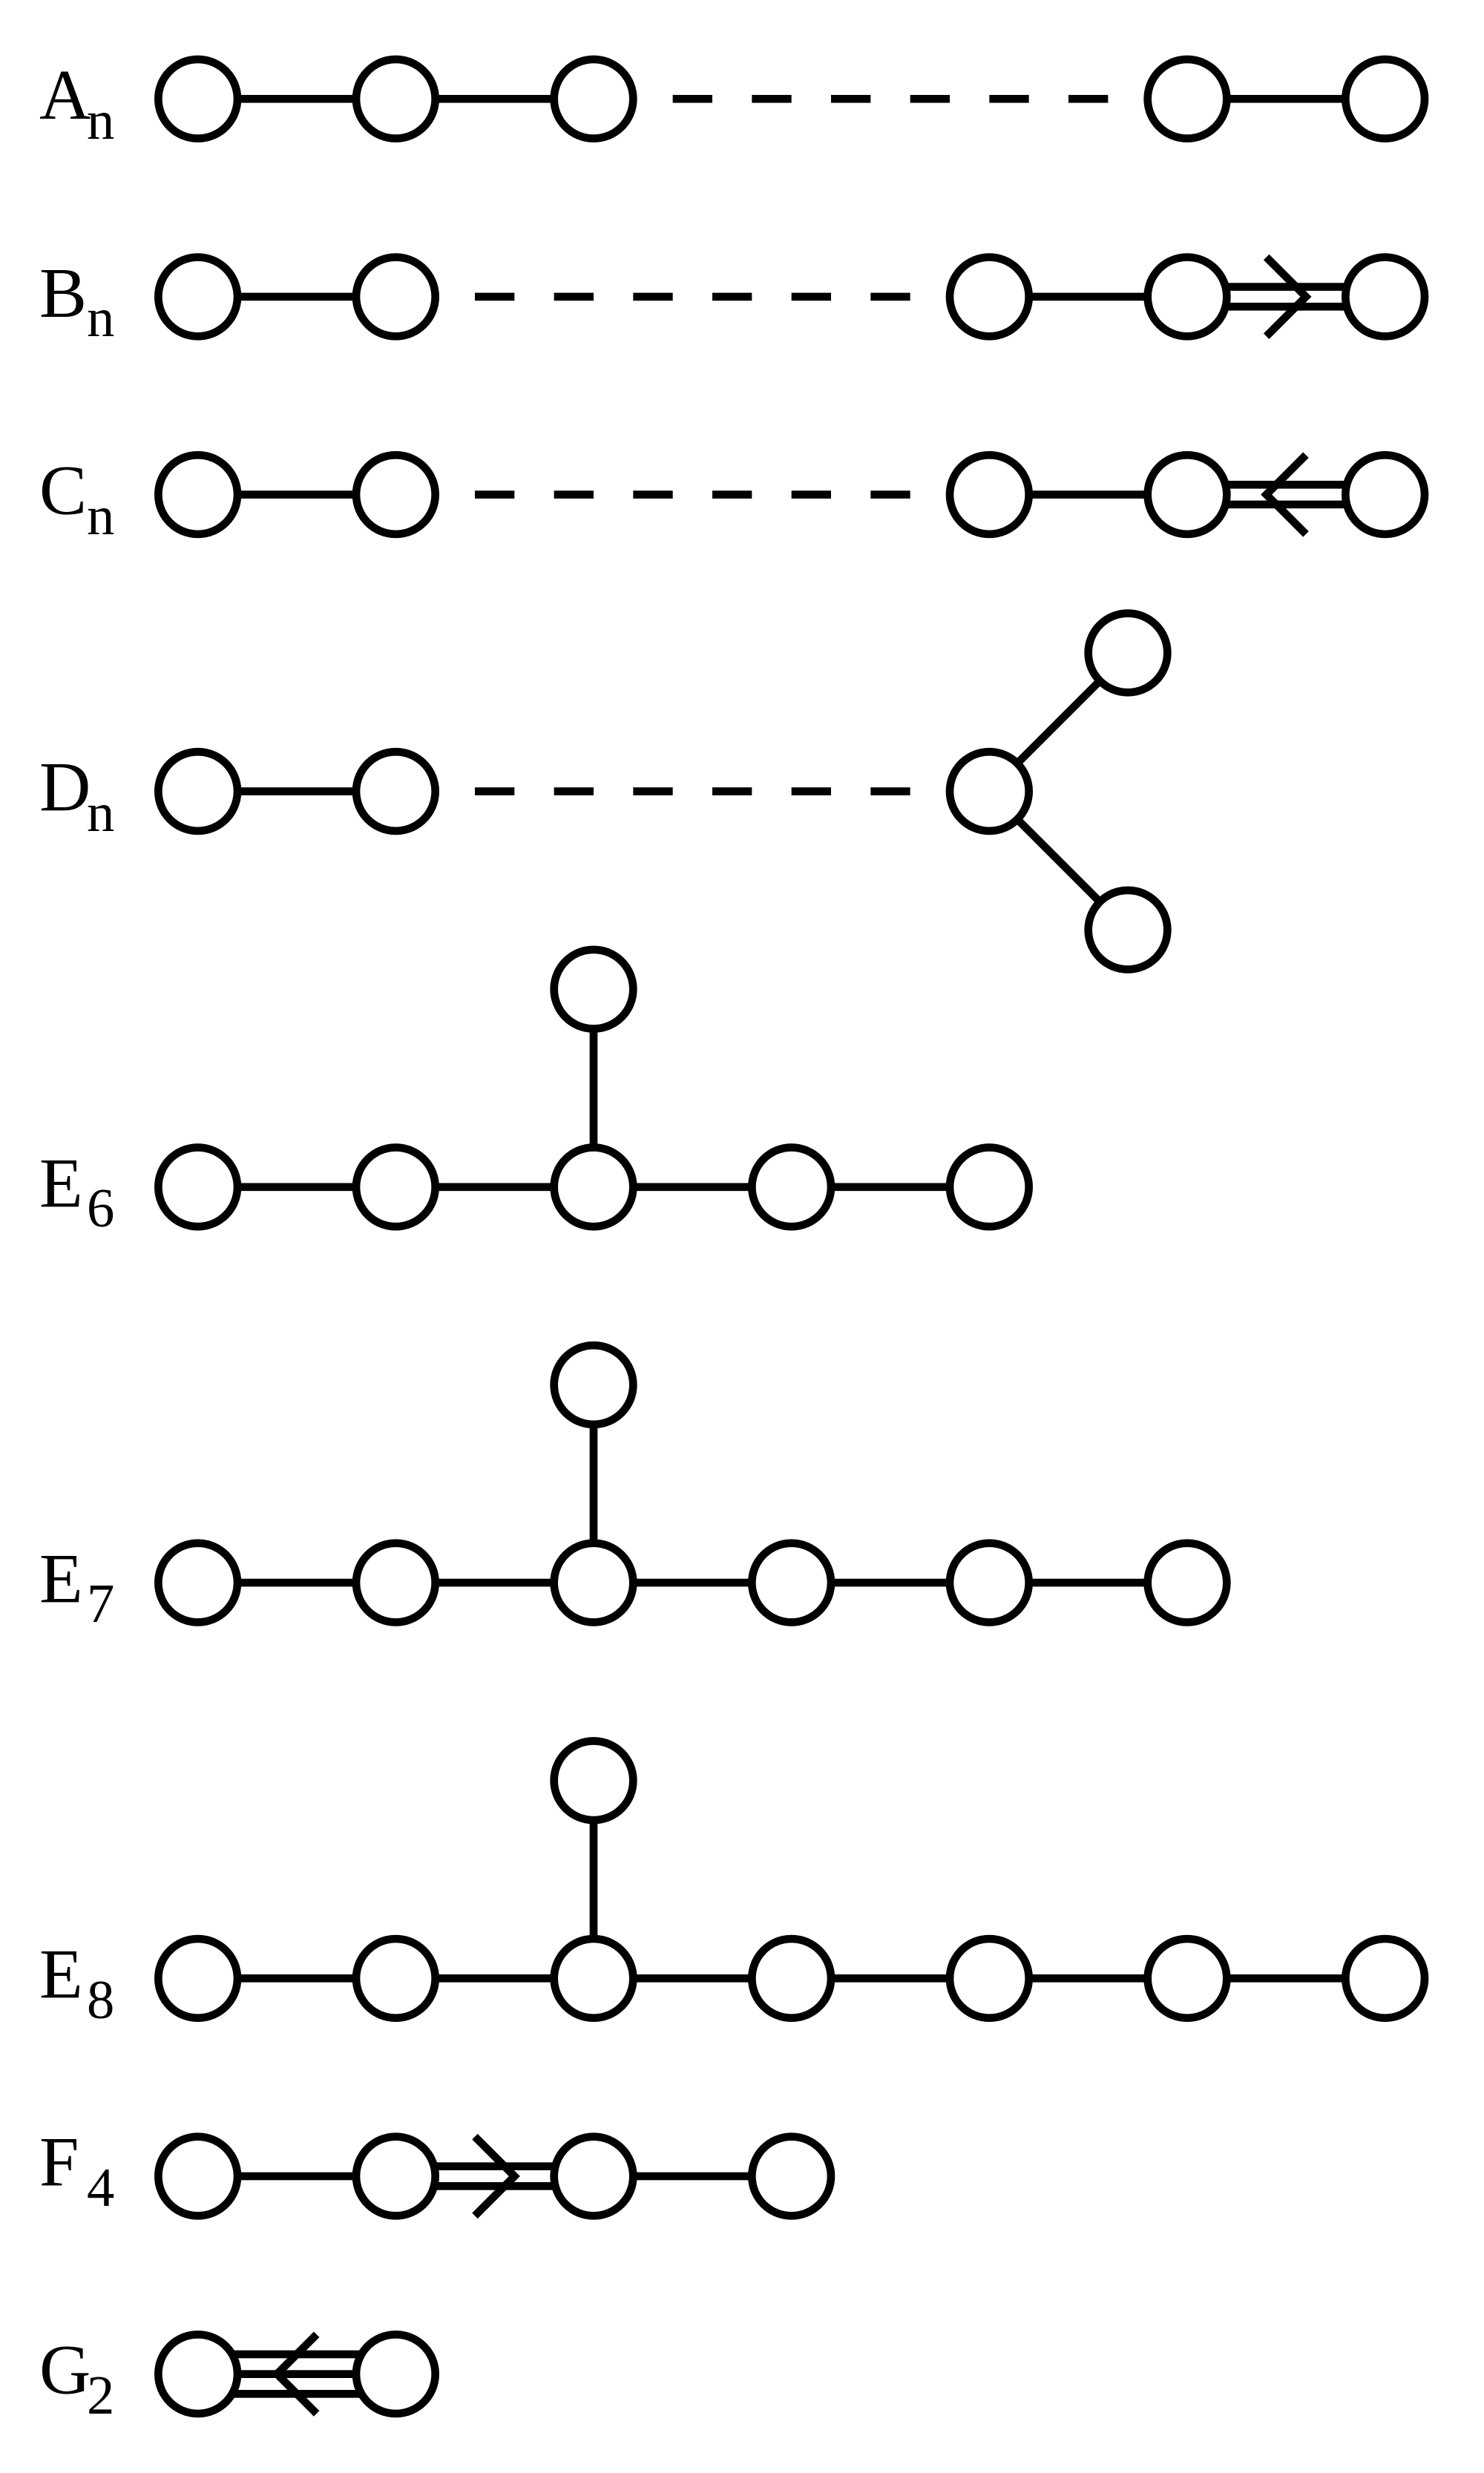
\includegraphics[scale=0.1]{sources/connected_dynkin_diagrams}
\end{figure}

\section{Classification of connected Coxeter graphs}
\begin{enumerate}
\item Consider in an inner-product space a set $\set{\eps_i}_{i\in\brs{n}}$ of linearly independent unit vectors, and form the graph where a pair $\eps_i \neq \eps_j$ are connected by $4\prs{\eps_i, \eps_j}^2$ edges such that this is an integer in $\set{0,1,2,3}$, satisfying $\prs{\eps_i, \eps_j} \leq 0$.\\
Call such a system of vectors \stress{admissible}.

\begin{remark}
A basis of an irreducible root system gives us an admissible set of vectors.
\end{remark}

\begin{remark}
Every subset of an admissible system is admissible.\\
Graphically, given an admissible system $U$, if $U' \subseteq U$, its graph is the induced sub-graph with vertices in $U'$.
\end{remark}

\item
Given an admissible system $U = \set{\eps_i}_{i \in \brs{n}}$, the number of pairs connected by edges is at most $n-1$.

\begin{proof}
Let $\eps = \sum_{i \in [n]} \eps_i$, then $\eps \neq 0$ because $U$ is linearly independent. Compute
\begin{align*}
\prs{\eps,\eps} &= \prs{\sum_{i\in[n]} \eps_i,\sum_{i\in[n]} \eps_i} \\&= n+2\sum_{i<j} \prs{\eps_i, \eps_j} = \star \text{.}
\end{align*}
We have $4\prs{\eps_i, \eps_j}^2 \in \set{0,1,2,3}$ and so if $\prs{\eps_i, \eps_j} \neq 0$ then $2\prs{\eps_i,\eps_j} \leq - 1$.\\
Substituting in $\star$,
\begin{align*}
0 < \delta = \prs{\eps,\eps} \\&= n+\sum_{i < j} 2\prs{\eps_i, \eps_j} \\&\leq n - \#\set{i < j}{\text{$\eps_i$ and $\eps_j$ are connected by an edge}}
\end{align*}
Therefore \[\#\set{i < j}{\text{$\eps_i$ and $\eps_j$ are connected by an edge}} \leq n - \delta\]
and so
\[\#\set{i < j}{\text{$\eps_i$ and $\eps_j$ are connected by an edge}} \leq n-1 \text{,}\]
as required.
\end{proof}

\item There are no cycles involving at least $3$ vertices in the graph, because a cycle has $n$ vertices and $n$ edges, and looking at the induced sub-graph gives a contradiction to the previous part.

\item The number of edges incident to a given vertex is at most $3$.
\begin{proof}
Let $\eps \in U$ where $U$ is an admissible system. Let $\set{u_i}_{i \in [k]}$ be the distinct vertices to which $\eps$ is connected, in $1$, $2$, or $3$ edges.\\
These neighbours of $\eps$ cannot be connected, because that would form a (non-degenerate) cycle, contradicting the previous part.
So, $\prs{u_i}_{i \in \brs{k}}$ is an orthonormal set.\\
Let $u_0$ be a unit vector orthogonal to $\prs{u_i}_{i \in \brs{k}}$ in the space $V=\mrm{span}\set{\eps, u_1, \ldots, u_k}$.\footnote{Notice that the spanning set is a basis, because elements of $U$ are linearly independent.}\\
Now, $\eps \notin \mrm{span}\set{u_i}_{i \in [k]}$, due to independence, and so $\eps$ cannot be orthogonal to a unit vector orthogonal to $\mrm{span}\set{u_i}_{i \in [k]}$. I.e. $\prs{\eps, u_0} \neq 0$.
So, we represent $\eps$ in the orthonormal basis
\[\eps = \sum_{i = 0}^k \prs{\eps, u_i} u_i \text{.}\]
Now
\begin{align*}
1 &= \prs{\eps, \eps} \\&=
\sum_{i=0}^k \prs{\eps, u_i}^2 \\&\stackrel{\prs{\eps, u_0} \neq 0}{=}
\sum_{i \in [k]} \prs{\eps, u_i}^2
\end{align*}
and multiplying sides by $4$ we get
\[4 > \sum_{i \in [k]} 4\prs{\eps, u_i}^2 = \#\set{\text{edges that connect $\eps$ to $\set{u_i}_{i\in[k]}$}} \text{.}\]
\end{proof}

\item
By the above, the only connected graph with a triple edge is $G_2$.

\item Suppose that the graph contains a simple chain as a sub-graph.\\
Let $\eps = \sum_{i \in [k]} \eps_i$ and consider the system $U' = U \setminus \prs{\set{\eps_i}_{i \in [k]} \cup \set{\eps}}$. This is an admissible system, and $\eps$ has the induced inner product with any vertex that was connected to each $\eps_i$.

\begin{proof}
First, $\eps$ is a unit vector.
\begin{align*}
\prs{\eps,\eps} &= \prs{\sum_{i\in[k]} \eps_i,\sum_{i\in[k]} \eps_i} \\&=
k + \sum_{i<j} 2 \prs{\eps_i, \eps_j} \\&\stackrel{\dagger}{=} k - \prs{k-1} \\&= 1
\end{align*}
with $\dagger$ being true because we assume $\prs{\eps_i}_{i\in[k]}$ is a chain which means only $\prs{\eps_j, \eps_{j+1}} \neq 0$ with $4 \prs{\eps_j, \eps_{j+1}}^2 = 1$\footnote{as there's one edge between $\eps_j, \eps_{j+1}$} and $2\prs{\eps_j, \eps_{j+1}} = -1$\footnote{since this expression is negative}.\\
Clearly, $\eps$ is linearly independent of $U \setminus \set{\eps_i}_{i\in[k]}$.\\
To show that $U'$ is an admissible system, we have to show that $4\prs{\eps,u}^2 \in \set{0,1,2,3}$ for all $u \in U \setminus \set{\eps_i}_{i\in[k]}$.\\
Consider $\prs{\eps,u} = \sum_{i \in [k]} \prs{\eps_i, u}$, we claim that at least $k-1$ of these inner products are zero. This is true because otherwise $u$ is connected to at least two elements of the chain, and one gets a (non-degenerate) cycle, contradicting a previous result. So, if $u \perp \eps_i$ for all $i \in [k]$, clearly $u \perp \eps$. If $\exists i \in [k] \colon \prs{u, \eps_i} \neq 0$, then $i$ is determined uniquely and $\prs{\eps, u} = \prs{\eps_i, u}$.
\end{proof}

\item
A connected graph cannot contain any of the sub-graphs in figure \ref{impossibe_contianing_chain}.

\begin{figure}[h!]
\centering
\caption{Impossible graphs containing a chain.}
\label{impossibe_contianing_chain}
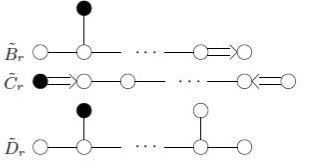
\includegraphics[scale=0.6]{sources/chain_contradiction}
\end{figure}

Otherwise, using the operation in the previous part we'd get the graphs in figure \ref{impossible_graphs}.
\begin{figure}[h!]
\centering
\caption{Impossible graphs.}
\label{impossible_graphs}
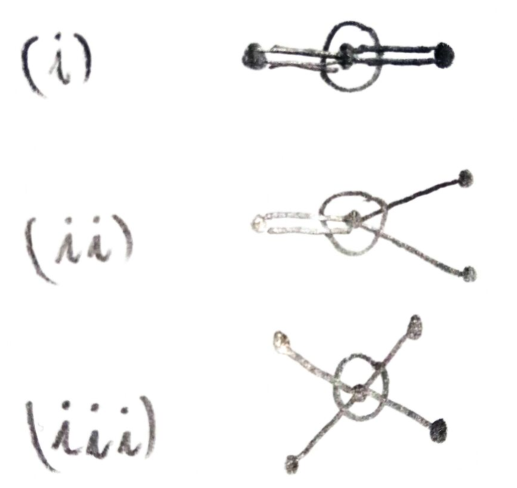
\includegraphics[scale=0.5]{sources/impossible}
\end{figure}
\begin{center}
\end{center}

respectively, each with a vertex connected to more than $3$ other vertices.

\item
All connected graph are of the following forms.
\begin{figure}[h!]
\centering
\caption{Possible graphs.}
\label{possible_graphs}
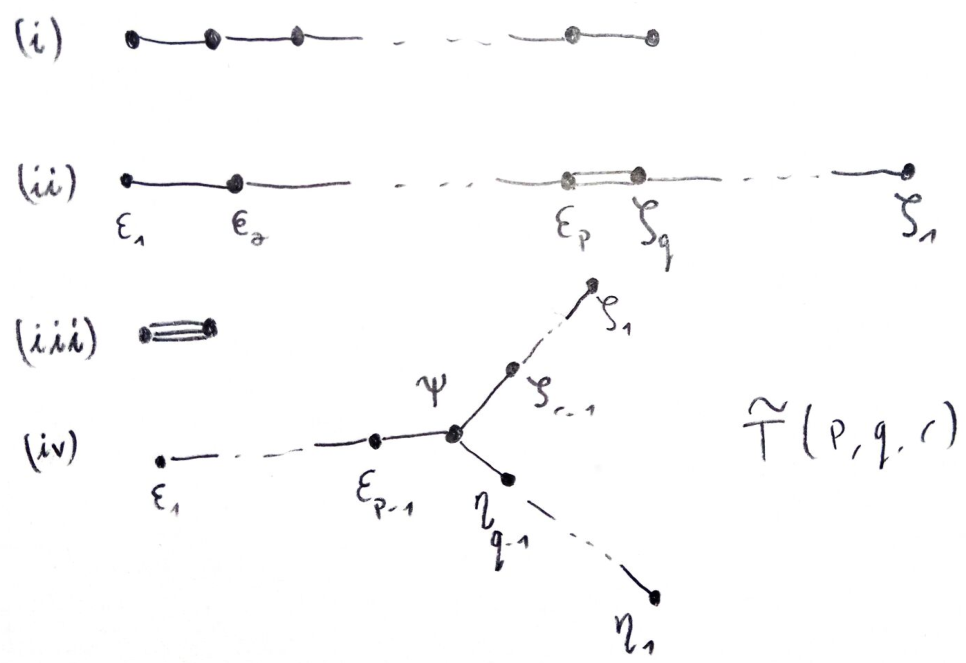
\includegraphics[scale=0.5]{sources/possible}
\end{figure}
\begin{center}
\end{center}

$G_2$ is the only connected with with a triple edge. See fig. \ref{possible_graphs}.
\begin{proof}
\begin{enumerate}[label = \Roman*)]
\item A double edge can appear only once. Otherwise we get the forbidden graph (i).
\item A tripod cannot appear together with a double edge, since this will give forbidden graph (ii).
\item A tripod can appear only once, since otherwise we get forbidden graph (iii).
\end{enumerate}
\end{proof}

\item Consider the graph $\tilde{B}\prs{p,q}$, in fig. \ref{possible_graphs}.
\\
Consider $\eps = \sum_{i \in [p]} i \eps _i$ and $\zeta = \sum_{j\in[q]} j \zeta_j$. Then
\begin{align*}
\prs{\eps, \eps} &= \sum_{i \in [p]} i^2 - \sum_{i\in[p-1]} i\prs{i+1}
\end{align*}
since $2 \prs{\eps_i, \eps_{i+1}} = -1$ and $\prs{\eps_i, \eps_j} = 0$ for $\abs{i-j} \geq 2$.\\
This yields $\prs{\eps,\eps} = \frac{p\prs{p+1}}{2}$, and similarly $\prs{\zeta, \zeta} = \frac{q\prs{q+1}}{2}$.\\
In the two chains, only $\eps,_p$ and $\zeta_q$ are connected, so
\begin{align*}
\prs{\eps, \zeta} &= 
\prs{\sum_{i \in [p]} i \eps_i, \sum_{j \in [q]} j \zeta_j} \\&=
\prs{p \eps_p, q\zeta_q} \\&=
pq \prs{\eps_p, \zeta_q}
\end{align*}
and so
\[\prs{\eps,\zeta}^2 = \frac{p^2 q^2}{4} 4\prs{\eps_p, \zeta_q}^2 = p^2 q^2\]
since $\eps_p,\zeta_q$ are connected by $2$ edges.\\
$\eps$ and $\zeta$ are linearly independent, and by Cauchy-Schwartz
\[\prs{\eps,\zeta}^2 < \prs{\eps,\eps} \prs{\zeta,\zeta} \text{.}\]
So,
\[\frac{p^2 q^2}{2} < \frac{p\prs{p+1}}{2} \frac{q\prs{q+1}}{2} \text{.}\]
Hence
\[pq < \frac{\prs{p+1}\prs{q+1}}{2} = \frac{1}{2}\prs{pq + p+q+1} \text{.}\]
Then
\[\frac{1}{2} pq - \frac{1}{2} p - \frac{1}{2} q < \frac{1}{2}\]
and then
\[\prs{p-1}\prs{q-1} < 2 \text{.}\]
Either $p=q=2$, in which case we get $F_4$, or $q=1$ and $p$ is arbitrary, in which case we get $B_{\ell}$.

\item
We show that in case (iv) we have \emph{only} $D_{\ell}$, $E_6$, $E_7$, or $E_8$.\footnote{We assume $r,q,p \geq 2$, because otherwise there is no tripod.}
\begin{proof}
Define the following vectors.
\begin{align*}
\eps &= \sum_{i \in [p-1]} i \eps_i \\
\eta &= \sum_{j \in [q-1]} j \eta_j \\
\zeta &= \sum_{k \in [r-1]} k \zeta_k
\end{align*}
$\set{\eps,\eta,\zeta,\psi}$ are linearly independent.\\
Let $\tau$ be a unit vector orthogonal to $\set{\eps,\eta,\zeta}$ in the space $\mrm{span}\set{\eps,\eta,\zeta,\psi}$. So, $\prs{\psi,\tau} \neq 0$.\\
$\set{\eps,\eta,\zeta,\tau}$ is an orthogonal basis of this space, because clearly $\set{\eps,\eta,\zeta}$ is orthogonal.\\
Write
\[\psi = \frac{\prs{\psi,\eps}}{\prs{\eps,\eps}^{\frac{1}{2}}}\eps + \frac{\prs{\psi,\eta}}{\prs{\eta,\eta}^{\frac{1}{2}}}\eta + \frac{\prs{\psi,\zeta}}{\prs{\zeta,\zeta}^{\frac{1}{2}}} \zeta + \prs{\psi,\tau} \tau \text{.}\]
Now $\prs{\psi,\psi} = 1$ because $\psi$ is in the system.\\
So,
\[\frac{\prs{\psi,\eps}}{\prs{\eps,\eps}^{\frac{1}{2}}}\eps + \frac{\prs{\psi,\eta}}{\prs{\eta,\eta}^{\frac{1}{2}}}\eta + \frac{\prs{\psi,\zeta}}{\prs{\zeta,\zeta}^{\frac{1}{2}}} \zeta < 1 \text{.}\]
As before,
\begin{align*}
\prs{\eps,\eps} &= \frac{p\prs{p-1}}{2} \\
\prs{\eta,\eta} &= \frac{q\prs{q-1}}{2} \\
\prs{\zeta,\zeta} &= \frac{r\prs{r-1}}{2} \text{.}
\end{align*}
We now compute.
\begin{align*}
4\prs{\psi,\eps} &= 4\prs{\psi, \sum_{i \in [p-1} i \eps_i}^2 \\&=
4\prs{\psi, \prs{p-1} \eps_{p-1}}^2 \\&=
\prs{p-1}^2 4\prs{\psi, \eps_{p-1}}^2 \\&=
\prs{p-1}^2
\end{align*}
so,
\[\frac{\prs{\psi,\eps}^2}{\prs{\eps,\eps}} = \frac{\frac{\prs{p-1}^2}{4}}{\frac{p\prs{p-1}}{2}} = \frac{1}{2} \frac{p-1}{p} = \frac{1}{2} \prs{1 - \frac{1}{p}} \text{.}\]
Similarly for the other two, so we conclude that
\[\frac{1}{2} \prs{1 - \frac{1}{p}} + \frac{1}{2} \prs{1 - \frac{1}{q}} + \frac{1}{2} \prs{1-\frac{1}{r}} < 1\text{.}\]
Multiplying by $2$,
\[3 - \prs{\frac{1}{p} + \frac{1}{q} + \frac{1}{r}} < 2\]
and so
\[\frac{1}{p} + \frac{1}{q} + \frac{1}{r} > 1 \text{.}\]
\begin{exercise}
The solutions to the above equation are
\begin{align*}
D_n &= \prs{p,2,2} \\
E_6 &= \prs{3,3,2} \\
E_7 &= \prs{4,3,2} \\
E_8 &= \prs{5,3,2} \text{.}
\end{align*}
\end{exercise}
\end{proof}
\end{enumerate}

\backmatter
\end{document}